



Number theory begins with the integers, and the single most important fact about the integers is that every one of them factors into primes in exactly one way. An enormous amount of elementary number theory is really just this statement being pushed around. So it is natural, when we want to solve an equation like $y^2 + 2 = x^3$ or $x^2 + y^2 = p$, to enlarge $\Z$ a little -- to work in $\Z[\sqrt{-2}]$ or $\Z[i]$ -- and hope that unique factorisation survives the move. Sometimes it does, and then the equation falls apart in a few lines. The trouble is that usually it does not: in $\Z[\sqrt{-5}]$ we have the notorious
$$6 = 2 \cdot 3 = (1 + \sqrt{-5})(1 - \sqrt{-5}),$$
and all four factors are irreducible. Unique factorisation of \emph{elements} is simply false in general.

The great insight, due to Kummer and then Dedekind, is that nothing is really lost -- we were just looking at the wrong objects. If instead of elements we factor \emph{ideals}, unique factorisation comes back, exactly and in complete generality, in the ring of integers of any number field. The extent to which ideals fail to be principal -- that is, the extent to which the ideal-theoretic picture differs from the element-theoretic one -- is measured by a finite abelian group, the \vocab{class group}, and computing this group for a given field is one of the central occupations of the subject. The other central object is the group of units, whose structure is pinned down by Dirichlet's unit theorem and which is intimately bound up with Pell's equation.

Both of the two big finiteness theorems -- finiteness of the class group, and the rank of the unit group -- are proved by the same startling device: we embed our number field into a Euclidean space so that its ring of integers becomes a \emph{lattice}, and then apply a piece of convex geometry due to Minkowski. Arithmetic questions become questions about counting lattice points in convex bodies. That this works at all is one of the small miracles of mathematics.

This article constitutes my notes for the `Number Fields' course, held in Lent 2022 at Cambridge. These notes are \emph{not a transcription of the lectures}, and differ significantly in quite a few areas. Still, all lectured material should be covered.



\section{Introduction}

\subsection{A Motivating Problem}

Which integers can be written as $x^2+y^2$? The answer is classical and completely satisfying: an odd prime $p$ is a sum of two squares exactly when $p \equiv 1 \pmod 4$. The slick proof, which we will give properly in Section \ref{sec:applications}, goes as follows. Factor
$$p = x^2+y^2 = (x+iy)(x-iy)$$
in the ring $\Z[i]$ of Gaussian integers. This ring turns out to be Euclidean, hence a principal ideal domain, hence a unique factorisation domain; and in a UFD one can chase the factorisation of $p$ around and read off the answer from whether $-1$ is a square mod $p$.

Emboldened, we might ask: which integers are of the form $x^2+5y^2$? Now we would like to factor
$$n = x^2+5y^2 = \left(x+y\sqrt{-5}\right)\left(x-y\sqrt{-5}\right)$$
in $\Z[\sqrt{-5}]$, and the argument collapses -- because $\Z[\sqrt{-5}]$ is \emph{not} a unique factorisation domain:
$$6 = 2 \cdot 3 = \left(1+\sqrt{-5}\right)\left(1-\sqrt{-5}\right),$$
with all four factors irreducible and no two associate. This is a genuine obstruction, not an artefact of a bad proof, and understanding it is the whole point of this course.

\subsection{Kummer's Idea}

The resolution, due to Kummer in the 1840s and refined by Dedekind, is that unique factorisation has not really failed: we have simply been factoring the wrong objects. Kummer imagined `ideal numbers' -- hypothetical divisors, not present in the ring, which would refine $2$, $3$ and $1\pm\sqrt{-5}$ into common building blocks. Dedekind made this precise by replacing an ideal number with the set of things it divides, that is, with an \emph{ideal} of the ring. In $\Z[\sqrt{-5}]$ the relevant ideals are
$$\fp = \left(2, 1+\sqrt{-5}\right), \qquad \fq_1 = \left(3,1+\sqrt{-5}\right), \qquad \fq_2 = \left(3, 1-\sqrt{-5}\right),$$
and one computes that
$$(2) = \fp^2, \quad (3) = \fq_1\fq_2, \quad \left(1+\sqrt{-5}\right) = \fp\fq_1, \quad \left(1-\sqrt{-5}\right) = \fp\fq_2.$$
So the two apparently different factorisations of $6$ are both the same factorisation
$$(6) = \fp\cdot\fp\cdot\fq_1\cdot\fq_2,$$
merely bracketed in two ways. Unique factorisation was there all along; it just could not be seen at the level of elements. The main theorem of Section \ref{sec:ideals} is that this always happens: in the ring of integers of \emph{any} number field, every nonzero ideal factors uniquely into prime ideals.

Of course, we then want to know how badly the ideals fail to be principal -- because that is what stops us from converting statements about ideals back into statements about elements. The answer is a group, the class group, and one of the two big theorems of the course is that it is finite.

\subsection{What We Will Do}

The plan of the course is as follows.
\begin{itemize}
	\item Sections \ref{sec:alg}--\ref{sec:normtrace} set up the basic objects: number fields $K$, their rings of integers $\OO_K$, and the numerical invariants attached to them -- norms, traces, integral bases and the discriminant $d_K$.
	\item Sections \ref{sec:ideals}--\ref{sec:idealnorm} develop the ideal theory: $\OO_K$ is a Dedekind domain, ideals factor uniquely into primes, and the failure of principality is measured by $\Cl_K$.
	\item Section \ref{sec:ram} answers the question `what are the prime ideals?'. They all sit above rational primes, and Dedekind's criterion reduces finding them to factoring a polynomial mod $p$. The primes that behave badly -- the \emph{ramified} ones -- are exactly the divisors of $d_K$.
	\item Section \ref{sec:geom} is the geometric heart. We embed $\OO_K$ into $\R^n$ as a lattice and apply Minkowski's convex body theorem to deduce that $\Cl_K$ is finite, with an explicit bound. Section \ref{sec:computing} puts this to work computing class groups.
	\item Section \ref{sec:units} determines the unit group $\OO_K^\times$ by the same geometric method: Dirichlet's unit theorem. In the real quadratic case this is the theory of Pell's equation.
	\item Section \ref{sec:applications} solves some Diophantine equations, and Section \ref{sec:zeta} (non-examinable) shows how the class number and the regulator appear together as the residue of the Dedekind zeta function.
\end{itemize}

Throughout, the reader should keep two examples in mind: the quadratic fields $\Q(\sqrt d)$, where everything can be computed by hand, and the cyclotomic fields $\Q(\zeta_m)$, which are where the subject came from and where it is still headed.

\section{Algebraic Integers}\label{sec:alg}

\subsection{Number Fields}

We will work throughout with finite extensions of $\Q$. Recall from Galois Theory that if $K \subseteq L$ are fields with $\dim_K L < \infty$, we write $[L:K]$ for this dimension and call $L/K$ a finite extension; every element of $L$ is then algebraic over $K$.

\begin{definition}[Number Field]
	A \vocab{number field} is a finite extension of $\Q$. Its \vocab{degree} is $[K:\Q]$.
\end{definition}

So $\Q$, $\Q(i)$, $\Q(\sqrt{2})$, $\Q(\sqrt[3]{2})$ and $\Q(\zeta_5)$ are all number fields, of degrees $1, 2, 2, 3$ and $4$ respectively. Since $\Q$ has characteristic zero, every number field is a separable extension of $\Q$, and so by the primitive element theorem every number field has the form $K = \Q(\alpha)$ for a single $\alpha$. We will use this constantly.

Inside $\Q$ sits $\Z$, and it is the arithmetic of $\Z$ that we care about. What we want, then, is the analogue of $\Z$ inside a general number field $K$. There is an obvious wrong answer -- take everything that is a root of \emph{some} polynomial over $\Q$, which gives all of $K$ -- and the correct answer comes from insisting on \emph{monic integer} polynomials.

\begin{definition}[Algebraic Integer]
	Let $K$ be a number field. An element $\alpha \in K$ is an \vocab{algebraic integer} if there is a monic polynomial $f \in \Z[x]$ with $f(\alpha) = 0$. We write
	$$\OO_K = \{\alpha \in K : \alpha \text{ is an algebraic integer}\}$$
	for the set of algebraic integers of $K$, called the \vocab{ring of integers} of $K$.
\end{definition}

Calling $\OO_K$ a ring is jumping the gun -- that it is closed under addition and multiplication is the first thing we have to prove, and it is not obvious. But let us first make sure that the definition does the right thing over $\Q$.

\begin{lemma}\label{lem:OQ}
	$\OO_\Q = \Z$.
\end{lemma}

\begin{proof}
	If $a \in \Z$ then $x - a$ is monic with integer coefficients and kills $a$, so $\Z \subseteq \OO_\Q$. Conversely suppose $\alpha = r/s \in \Q$ with $r, s$ coprime and $s \geq 1$, and suppose
	$$\alpha^n + a_{n-1}\alpha^{n-1} + \dots + a_0 = 0$$
	with all $a_i \in \Z$. Multiplying through by $s^n$ gives
	$$r^n = -s\left(a_{n-1}r^{n-1} + a_{n-2}r^{n-2}s + \dots + a_0 s^{n-1}\right),$$
	so $s \mid r^n$. If $s > 1$, pick a prime $p \mid s$; then $p \mid r^n$, so $p \mid r$, contradicting coprimality. Hence $s = 1$ and $\alpha \in \Z$.
\end{proof}

This is a reassuring start, and it also explains a piece of terminology: elements of $\Z$ are sometimes called \vocab{rational integers} when we need to distinguish them from algebraic integers. The picture to keep in mind is a square, with $\OO_K$ playing the role for $K$ that $\Z$ plays for $\Q$.

\begin{center}
	\begin{tikzpicture}[scale=1.2]
		\node (Z) at (0,0) {$\Z$};
		\node (Q) at (2.2,0) {$\Q$};
		\node (O) at (0,1.5) {$\OO_K$};
		\node (K) at (2.2,1.5) {$K$};
		\draw[right hook->] (Z) -- (Q);
		\draw[right hook->] (O) -- (K);
		\draw[right hook->] (Z) -- (O);
		\draw[right hook->] (Q) -- (K);
		\node at (1.1,-0.42) {\small field of fractions};
		\node at (1.1,1.92) {\small field of fractions};
	\end{tikzpicture}
\end{center}

We will justify both `field of fractions' labels shortly. Note straight away that $\alpha \in \OO_K$ does \emph{not} imply $1/\alpha \in \OO_K$ -- for instance $2 \in \OO_\Q = \Z$ but $1/2 \notin \Z$. Understanding exactly which $\alpha$ have $1/\alpha \in \OO_K$ is the theory of units, which we take up in Section \ref{sec:units}.

\subsection{Integrality}

The obstacle to showing $\OO_K$ is a ring is that the Galois-theoretic argument -- that $\alpha \pm \beta$ and $\alpha\beta$ are algebraic whenever $\alpha, \beta$ are -- produces polynomials that need not be monic over $\Z$. We need a genuinely different idea, and the right one is a piece of commutative algebra which we may as well set up in general.

\begin{definition}[Integral]
	Let $R \subseteq S$ be commutative rings with $1$.
	\begin{enumerate}[label=(\roman*)]
		\item An element $\alpha \in S$ is \vocab{integral over $R$} if there is a monic $f \in R[x]$ with $f(\alpha) = 0$.
		\item $S$ is \vocab{integral over $R$} if every $\alpha \in S$ is integral over $R$.
		\item $S$ is \vocab{finitely generated as an $R$-module} if there are $\alpha_1, \dots, \alpha_n \in S$ such that every element of $S$ is an $R$-linear combination of the $\alpha_i$; equivalently, the map $R^n \to S$, $(r_1,\dots,r_n) \mapsto \sum r_i\alpha_i$, is surjective.
	\end{enumerate}
\end{definition}

So $\alpha \in K$ is an algebraic integer precisely when it is integral over $\Z$. If $\alpha_1, \dots, \alpha_r \in S$ we write $R[\alpha_1, \dots, \alpha_r]$ for the subring of $S$ generated by $R$ and the $\alpha_i$; this is the image of the evaluation map $R[x_1,\dots,x_r] \to S$ sending $x_i \mapsto \alpha_i$. Beware that being finitely generated as a \emph{module} is much stronger than being finitely generated as a \emph{ring}: $\Z[x]$ is generated as a ring by one element over $\Z$, but is very far from being a finitely generated $\Z$-module.

The two notions are linked by the following pair of results, and the link is the whole point.

\begin{proposition}\label{prop:intfg}
	Let $R \subseteq S$ be rings and let $s \in S$ be integral over $R$. Then $R[s]$ is a finitely generated $R$-module. More generally, if $s_1, \dots, s_n \in S$ are each integral over $R$, then $R[s_1, \dots, s_n]$ is a finitely generated $R$-module.
\end{proposition}

\begin{proof}
	The ring $R[s]$ is spanned as an $R$-module by $1, s, s^2, \dots$. By hypothesis there are $a_0, \dots, a_{n-1} \in R$ with $s^n = a_{n-1}s^{n-1} + \dots + a_0$. Let $M = R \cdot 1 + Rs + \dots + Rs^{n-1}$. Then $sM \subseteq M$: indeed $s \cdot s^i = s^{i+1} \in M$ for $i < n-1$, and $s\cdot s^{n-1} = s^n \in M$ by the displayed relation. Hence $M$ contains $s^n, s^{n+1}, \dots$ by induction, so $M = R[s]$, which is therefore generated by the $n$ elements $1, s, \dots, s^{n-1}$.

	For the general statement, first note the transitivity of finite generation: if $A \subseteq B \subseteq C$ with $B$ a finitely generated $A$-module, say with generators $b_i$, and $C$ a finitely generated $B$-module, say with generators $c_j$, then the products $b_ic_j$ generate $C$ as an $A$-module. Now put $S_i = R[s_1,\dots,s_i]$, so $S_0 = R$ and $S_{i+1} = S_i[s_{i+1}]$. Each $s_{i+1}$ is integral over $R$ and hence over the larger ring $S_i$, so $S_{i+1}$ is a finitely generated $S_i$-module by the first part. Transitivity gives the result.
\end{proof}

Now for the converse direction, which is the clever one. The proof is essentially the proof of the Cayley--Hamilton theorem, and it is worth appreciating that it is entirely constructive: it hands us the monic polynomial explicitly, as a characteristic polynomial.

\begin{theorem}\label{thm:fgint}
	Let $R \subseteq S$ be rings with $S$ a finitely generated $R$-module. Then $S$ is integral over $R$.
\end{theorem}

\begin{proof}
	Let $\alpha_1, \dots, \alpha_n$ generate $S$ as an $R$-module; since $1 \in S$ we may assume that $\alpha_1 = 1$ after enlarging the generating set. Fix $s \in S$. Each $s\alpha_i$ lies in $S$, so we may write
	$$s\alpha_i = \sum_{j=1}^n b_{ij}\alpha_j$$
	for some $b_{ij} \in R$. Setting $B = (b_{ij}) \in \mathrm{Mat}_n(R)$ and $v = (\alpha_1, \dots, \alpha_n)^T$, this says
	$$(sI - B)\,v = 0.$$
	Recall that for any square matrix $X$ over a commutative ring we have $\adj(X)\,X = (\det X) I$. Multiplying on the left by $\adj(sI - B)$ therefore gives $\det(sI - B)\, v = 0$; looking at the first coordinate and using $\alpha_1 = 1$ yields
	$$\det(sI - B) = 0.$$
	But $f(t) = \det(tI - B)$ is a monic polynomial of degree $n$ with coefficients in $R$, and $f(s) = 0$. So $s$ is integral over $R$.
\end{proof}

Combining the two results gives exactly what we wanted.

\begin{corollary}\label{cor:OKring}
	Let $K$ be a number field. Then $\OO_K$ is a subring of $K$.
\end{corollary}

\begin{proof}
	Let $\alpha, \beta \in \OO_K$. By Proposition \ref{prop:intfg}, $\Z[\alpha,\beta]$ is a finitely generated $\Z$-module, so by Theorem \ref{thm:fgint} every element of $\Z[\alpha,\beta]$ is integral over $\Z$. In particular $\alpha \pm \beta$ and $\alpha\beta$ are algebraic integers, and $0, 1 \in \OO_K$ trivially.
\end{proof}

The same argument gives transitivity of integrality, which we will want later.

\begin{corollary}[Transitivity of Integrality]\label{cor:transint}
	Let $A \subseteq B \subseteq C$ be rings with $B$ integral over $A$ and $C$ integral over $B$. Then $C$ is integral over $A$.
\end{corollary}

\begin{proof}
	Let $c \in C$ and let $c^n + b_{n-1}c^{n-1} + \dots + b_0 = 0$ with $b_i \in B$. Put $B_0 = A[b_0, \dots, b_{n-1}]$ and $C_0 = B_0[c]$. Then $B_0$ is a finitely generated $A$-module, since each $b_i$ is integral over $A$; and $C_0$ is a finitely generated $B_0$-module, since $c$ is integral over $B_0$ (the displayed relation has coefficients in $B_0$). By transitivity of finite generation, $C_0$ is a finitely generated $A$-module, so Theorem \ref{thm:fgint} shows $c$ is integral over $A$.
\end{proof}

\begin{remark}
	The passage to the finitely generated subring $C_0$ is essential: $C$ itself might be enormous. For example the set of \emph{all} algebraic integers in $\C$ is a ring which is integral over $\Z$, but it is nowhere near being a finitely generated $\Z$-module. This kind of manoeuvre -- reduce to a finitely generated situation, then apply the determinant trick -- is one of the standard moves of commutative algebra, and it is worth internalising.
\end{remark}

\subsection{Minimal Polynomials}

To decide whether a given $\alpha$ is an algebraic integer, we would rather not have to hunt for a monic integer polynomial. Happily we do not have to: it is enough to look at the minimal polynomial.

Recall that for $\alpha$ algebraic over a field $K$, the \vocab{minimal polynomial} $p_\alpha \in K[x]$ is the monic polynomial of least degree with $p_\alpha(\alpha) = 0$, and that it divides every polynomial in $K[x]$ killing $\alpha$ (divide with remainder and use minimality); in particular it is unique and irreducible.

\begin{proposition}\label{prop:minpolyZ}
	Let $K$ be a number field and $\alpha \in K$, with minimal polynomial $p_\alpha \in \Q[x]$. Then $\alpha \in \OO_K$ if and only if $p_\alpha \in \Z[x]$.
\end{proposition}

\begin{proof}
	If $p_\alpha \in \Z[x]$ then $\alpha$ is integral over $\Z$ by definition, since $p_\alpha$ is monic.

	Conversely suppose $\alpha \in \OO_K$, say $h(\alpha) = 0$ with $h \in \Z[x]$ monic. Then $p_\alpha \mid h$ in $\Q[x]$. Let $M$ be a splitting field for $p_\alpha$ containing $K$, and let $\alpha_1, \dots, \alpha_m \in M$ be the roots of $p_\alpha$. Each $\alpha_i$ is a root of $h$, hence is an algebraic integer. But the coefficients of $p_\alpha = \prod_i (x - \alpha_i)$ are (up to sign) the elementary symmetric functions of the $\alpha_i$, hence are algebraic integers by Corollary \ref{cor:OKring} applied in $M$. They also lie in $\Q$, so by Lemma \ref{lem:OQ} they lie in $\Z$.
\end{proof}

\begin{remark}
	There is a second proof, from IB Groups, Rings and Modules: $p_\alpha$ is monic and divides the monic integer polynomial $h$ in $\Q[x]$, so writing $h = p_\alpha g$ with $g \in \Q[x]$ monic, Gauss's lemma forces both $p_\alpha$ and $g$ to lie in $\Z[x]$. Either argument is fine; the first has the advantage of not needing $h$ to be around.
\end{remark}

This makes it easy to check membership of $\OO_K$ in practice. For example $\tfrac{1}{2}(1 + \sqrt{5})$ has minimal polynomial $x^2 - x - 1 \in \Z[x]$, so it is an algebraic integer, whereas $\tfrac{1}{2}(1 + \sqrt{3})$ has minimal polynomial $x^2 - x - \tfrac12 \notin \Z[x]$ and so is not.

We can also now justify the `field of fractions' claim from the picture above. The point is that any element of $K$ becomes an algebraic integer after multiplication by a suitable rational integer -- we can always clear denominators.

\begin{lemma}\label{lem:clear}
	Let $K$ be a number field and $\alpha \in K$. Then there is a nonzero $n \in \Z$ with $n\alpha \in \OO_K$. Consequently $\Frac(\OO_K) = K$.
\end{lemma}

\begin{proof}
	Let $g(x) = x^m + c_{m-1}x^{m-1} + \dots + c_0 \in \Q[x]$ be the minimal polynomial of $\alpha$, and choose $n \in \Z_{>0}$ with $nc_i \in \Z$ for all $i$. Then
	$$h(x) = n^m g\!\left(\frac{x}{n}\right) = x^m + nc_{m-1}x^{m-1} + n^2c_{m-2}x^{m-2}+\dots+n^m c_0$$
	is monic with integer coefficients (as $n^{m-i}c_i \in \Z$ for $i \le m-1$), and $h(n\alpha) = n^mg(\alpha) = 0$. So $n\alpha \in \OO_K$.

	For the consequence, $\Frac(\OO_K) \subseteq K$ is clear, and any $\alpha \in K$ can be written as $(n\alpha)/n$ with $n\alpha \in \OO_K$ and $n \in \Z \subseteq \OO_K$.
\end{proof}

\subsection{Quadratic Fields}

Before developing more theory it is worth computing $\OO_K$ in the simplest interesting case, both because we will use the answer constantly and because it already contains a surprise.

\begin{definition}[Quadratic Field]
	A \vocab{quadratic field} is a number field of degree $2$.
\end{definition}

Every quadratic field is of the form $\Q(\sqrt{d})$ for a unique squarefree $d \in \Z \setminus \{0,1\}$. Indeed if $[K:\Q] = 2$ and $\alpha \in K \setminus \Q$ then $K = \Q(\alpha)$ and $\alpha$ satisfies a quadratic over $\Q$; completing the square writes $K = \Q(\sqrt{c})$ for some $c \in \Q$, and scaling $c$ by squares of rationals reduces to squarefree $d \in \Z$. We call $K$ \vocab{real quadratic} if $d > 0$ and \vocab{imaginary quadratic} if $d < 0$.

\begin{lemma}\label{lem:quadOK}
	Let $d \in \Z$ be squarefree, $d \neq 0, 1$, and let $K = \Q(\sqrt d)$. Then
	$$\OO_K = \begin{cases} \Z[\sqrt d] & \text{if } d \equiv 2, 3 \pmod 4,\\[2pt] \Z\!\left[\tfrac{1}{2}(1+\sqrt d)\right] & \text{if } d \equiv 1 \pmod 4.\end{cases}$$
\end{lemma}

\begin{proof}
	Write $\alpha = x + y\sqrt d$ with $x, y \in \Q$. If $y = 0$ then $\alpha \in \OO_K$ iff $\alpha \in \Z$ by Lemma \ref{lem:OQ}. If $y \neq 0$ then the minimal polynomial of $\alpha$ is
	$$p_\alpha(t) = (t - x)^2 - dy^2 = t^2 - 2xt + (x^2 - dy^2),$$
	so by Proposition \ref{prop:minpolyZ}, $\alpha \in \OO_K$ if and only if $2x \in \Z$ and $x^2 - dy^2 \in \Z$.

	Suppose these hold. Then $4x^2 - 4dy^2 \in \Z$ and $4x^2 \in \Z$, so $4dy^2 \in \Z$. Write $y = r/s$ in lowest terms; then $s^2 \mid 4dr^2$, so $s^2 \mid 4d$, and as $d$ is squarefree this forces $s \mid 2$. So we may write $x = u/2$ and $y = v/2$ with $u, v \in \Z$, and the conditions become
	$$u^2 - dv^2 \equiv 0 \pmod 4.$$
	Squares are $0$ or $1$ mod $4$. If $u, v$ are both even we get $x, y \in \Z$. If $u$ is odd then $u^2 \equiv 1$, so we need $dv^2 \equiv 1 \pmod 4$, forcing $v$ odd and $d \equiv 1 \pmod 4$. If $u$ is even and $v$ odd then $d \equiv 0 \pmod 4$, impossible as $d$ is squarefree.

	So if $d \equiv 2, 3 \pmod 4$ we must have $u, v$ both even, giving $\OO_K = \Z \oplus \Z\sqrt d = \Z[\sqrt d]$. If $d \equiv 1 \pmod 4$ then $u \equiv v \pmod 2$ is exactly the condition, and $\{u/2 + (v/2)\sqrt d : u \equiv v \bmod 2\} = \Z \oplus \Z\cdot\tfrac12(1+\sqrt d)$, which is the ring $\Z[\tfrac12(1+\sqrt d)]$: note $\tfrac12(1+\sqrt d)$ has minimal polynomial $t^2 - t + \tfrac14(1-d) \in \Z[x]$ precisely because $d \equiv 1 \pmod 4$.
\end{proof}

The case $d \equiv 1 \pmod 4$ is the surprise: the naive guess $\Z[\sqrt d]$ is too small, and misses half of the integers. This will matter enormously.

\begin{example}
	Let us record the two most important cases.
	\begin{enumerate}[label=(\roman*)]
		\item $d = -1$: here $-1 \equiv 3 \pmod 4$, so $\OO_{\Q(i)} = \Z[i]$, the \vocab{Gaussian integers}. Embedded in $\C$ this is the square lattice.
		\item $d = -3$: here $-3 \equiv 1 \pmod 4$, so $\OO_{\Q(\sqrt{-3})} = \Z[\omega]$ where $\omega = \tfrac12(1 + \sqrt{-3}) = e^{i\pi/3}$. These are the \vocab{Eisenstein integers}, and embedded in $\C$ they form the triangular lattice -- strictly bigger than $\Z[\sqrt{-3}]$, which is a rectangular sublattice of index $2$.
	\end{enumerate}
	Here are the two pictures, drawn in $\C$.
	\begin{center}
		\begin{tikzpicture}[scale=0.72]
			\begin{scope}
				\clip (-2.45,-2.45) rectangle (2.45,2.45);
				\foreach \a in {-3,...,3}{
					\foreach \b in {-3,...,3}{
						\fill[blue] (\a,\b) circle (2pt);
					}
				}
			\end{scope}
			\draw[<->, gray!70] (-2.6,0) -- (2.6,0);
			\draw[<->, gray!70] (0,-2.6) -- (0,2.6);
			\draw[thick,blue] (0,0) -- (1,0) -- (1,1) -- (0,1) -- cycle;
			\node[below right] at (1,0) {\small $1$};
			\node[above left] at (0,1) {\small $i$};
			\node at (0,-3.2) {$\Z[i]$};
		\end{tikzpicture}
		\hspace{1.1cm}
		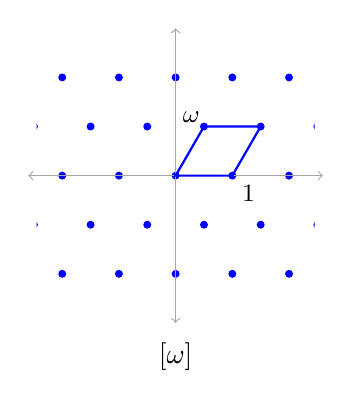
\begin{tikzpicture}[scale=0.72]
			\begin{scope}
				\clip (-2.45,-2.45) rectangle (2.45,2.45);
				\foreach \a in {-4,...,4}{
					\foreach \b in {-3,...,3}{
						\fill[blue] ({\a+0.5*\b},{0.8660*\b}) circle (2pt);
					}
				}
			\end{scope}
			\draw[<->, gray!70] (-2.6,0) -- (2.6,0);
			\draw[<->, gray!70] (0,-2.6) -- (0,2.6);
			\draw[thick,blue] (0,0) -- (1,0) -- (1.5,0.866) -- (0.5,0.866) -- cycle;
			\node[below right] at (1,0) {\small $1$};
			\node[above left=-2pt] at (0.5,0.866) {\small $\omega$};
			\node at (0,-3.2) {$\Z[\omega]$};
		\end{tikzpicture}
	\end{center}
	In both cases $\OO_K$ sits inside $\C$ as a lattice; that this always happens, in a suitable sense, is the content of Section \ref{sec:geom}.
\end{example}

\begin{example}
	$\OO_{\Q(\sqrt 5)} = \Z[\tfrac12(1+\sqrt5)] = \Z[\varphi]$, where $\varphi$ is the golden ratio, with $\varphi^2 = \varphi + 1$. On the other hand $\OO_{\Q(\sqrt 2)} = \Z[\sqrt2]$ and $\OO_{\Q(\sqrt{-5})} = \Z[\sqrt{-5}]$, since $2, 3 \equiv 2, 3 \pmod 4$.
\end{example}

\section{Norms, Traces and Discriminants}\label{sec:normtrace}

\subsection{The Norm and the Trace}

Two extremely useful invariants attach to an element of a field extension, and we met both in Galois Theory. The idea is to remember that $L$ is a vector space over $K$, and that multiplication by an element of $L$ is a $K$-linear map.

\begin{definition}[Norm and Trace]
	Let $L/K$ be a finite extension of degree $n$ and let $\alpha \in L$. Multiplication by $\alpha$,
	$$m_\alpha : L \to L, \qquad m_\alpha(y) = \alpha y,$$
	is a $K$-linear endomorphism. We define the \vocab{norm} and \vocab{trace} of $\alpha$ relative to $L/K$ by
	$$\Nm_{L/K}(\alpha) = \det(m_\alpha) \in K, \qquad \Tr_{L/K}(\alpha) = \tr(m_\alpha) \in K.$$
	When $K = \Q$ and $L$ is understood we simply write $\Nm(\alpha)$ and $\Tr(\alpha)$.
\end{definition}

Since $\alpha \mapsto m_\alpha$ is a $K$-algebra homomorphism $L \to \operatorname{End}_K(L)$, the norm is multiplicative and the trace is $K$-linear:
$$\Nm_{L/K}(\alpha\beta) = \Nm_{L/K}(\alpha)\Nm_{L/K}(\beta), \qquad \Tr_{L/K}(\alpha+\beta) = \Tr_{L/K}(\alpha) + \Tr_{L/K}(\beta).$$
Also $\Nm_{L/K}(\alpha) = 0$ if and only if $\alpha = 0$, so $\Nm_{L/K} : L^\times \to K^\times$ is a group homomorphism.

\begin{example}\label{ex:quadnormtrace}
	Let $L = K(\sqrt d)$ with $d \in K$ not a square, and let $\alpha = x + y\sqrt d$. In the basis $1, \sqrt d$ we have $\alpha \cdot 1 = x + y \sqrt d$ and $\alpha \cdot \sqrt d = dy + x\sqrt d$, so
	$$m_\alpha = \begin{pmatrix} x & dy \\ y & x\end{pmatrix},$$
	giving
	$$\Tr_{L/K}(x + y\sqrt d) = 2x, \qquad \Nm_{L/K}(x+y\sqrt d) = x^2 - dy^2.$$
	Notice that these are exactly $\alpha + \bar\alpha$ and $\alpha\bar\alpha$, where $\bar\alpha = x - y\sqrt d$ is the conjugate. For $d = -1$ the norm is the familiar $\abs{x+iy}^2$.
\end{example}

Recall from Galois Theory the relationship between $m_\alpha$ and the minimal polynomial: if $p_\alpha$ is the minimal polynomial of $\alpha$ over $K$, then the characteristic polynomial of $m_\alpha$ on $L$ is
$$\det(x I - m_\alpha) = p_\alpha(x)^{[L : K(\alpha)]}.$$
(The reason is that $L$ is a free $K(\alpha)$-module of rank $[L:K(\alpha)]$, and on $K(\alpha)$ with basis $1, \alpha, \dots, \alpha^{\deg p_\alpha - 1}$ the matrix of $m_\alpha$ is the companion matrix of $p_\alpha$.) Comparing coefficients gives, when $p_\alpha(t) = \prod_{i=1}^r (t - \alpha_i)$ splits in some extension,
$$\Nm_{L/K}(\alpha) = \left(\prod_{i=1}^r \alpha_i\right)^{[L:K(\alpha)]}, \qquad \Tr_{L/K}(\alpha) = [L:K(\alpha)]\sum_{i=1}^r \alpha_i.$$

This has an immediate consequence for algebraic integers, which will be our main computational tool for recognising them.

\begin{lemma}\label{lem:normtraceZ}
	Let $K$ be a number field and $\alpha \in \OO_K$. Then $\Nm_{K/\Q}(\alpha) \in \Z$ and $\Tr_{K/\Q}(\alpha) \in \Z$.
\end{lemma}

\begin{proof}
	By Proposition \ref{prop:minpolyZ} the minimal polynomial $p_\alpha$ has integer coefficients, and the characteristic polynomial of $m_\alpha$ is a power of $p_\alpha$, hence also lies in $\Z[x]$. The norm and trace are, up to sign, coefficients of this characteristic polynomial.
\end{proof}

\begin{remark}
	The converse is false in general, but true in the quadratic case: if $[K:\Q] = 2$ and $\alpha \in K \setminus \Q$, then the characteristic polynomial of $m_\alpha$ \emph{is} the minimal polynomial, and it equals $x^2 - \Tr(\alpha)x + \Nm(\alpha)$. So $\alpha \in \OO_K$ if and only if $\Tr(\alpha), \Nm(\alpha) \in \Z$. This is exactly what we used in the proof of Lemma \ref{lem:quadOK}.
\end{remark}

\subsection{Embeddings}

For number fields there is a much better description of the norm and trace, in terms of the embeddings into $\C$. Let $K = \Q(\theta)$ be a number field of degree $n$, with $\theta$ having minimal polynomial $p_\theta$ of degree $n$, so that $K \cong \Q[x]/(p_\theta)$ and $1, \theta, \dots, \theta^{n-1}$ is a $\Q$-basis of $K$.

\begin{lemma}\label{lem:nembeddings}
	There are exactly $n$ field embeddings $K \hookrightarrow \C$.
\end{lemma}

\begin{proof}
	As $p_\theta$ is irreducible over $\Q$ and $\Q$ has characteristic zero, $\gcd(p_\theta, p_\theta') = 1$, so $p_\theta$ has $n$ distinct roots $\theta_1, \dots, \theta_n \in \C$. A field homomorphism $\Q[x]/(p_\theta) \to \C$ is automatically $\Q$-linear, hence determined by the image of $x$, which must be a root of $p_\theta$; and each root gives such a homomorphism. These $n$ maps are distinct since they differ on $\theta$.
\end{proof}

Some of these embeddings land in $\R$ and some do not, and the ones that do not come in conjugate pairs since complex conjugation permutes the roots of a real polynomial.

\begin{definition}[Signature]
	Let $K$ be a number field of degree $n$. Let $r$ be the number of embeddings $K \hookrightarrow \R$ and let $s$ be the number of conjugate pairs of non-real embeddings $K \hookrightarrow \C$, so that $r + 2s = n$. We call $(r,s)$ the \vocab{signature} of $K$, and label the embeddings
	$$\sigma_1, \dots, \sigma_r : K \to \R, \qquad \sigma_{r+1}, \overline{\sigma_{r+1}}, \dots, \sigma_{r+s}, \overline{\sigma_{r+s}} : K \to \C.$$
\end{definition}

Since $r$ counts the real roots of $p_\theta$, and $r$ can also be described as the number of embeddings of $K$ into $\R$ (a description not mentioning $\theta$), the pair $(r,s)$ is an invariant of $K$ and not of the chosen generator. Here is the picture: the conjugates of $\theta$ sit in $\C$, some on the real axis and the rest in mirror-image pairs.

\begin{center}
	\begin{tikzpicture}[scale=0.95]
		\draw[<->, gray!70] (-3.1,0) -- (3.1,0) node[right, black] {\small $\R$};
		\draw[<->, gray!70] (0,-1.6) -- (0,1.6);
		\fill[blue] (-2.3,0) circle (2.1pt) node[below=3pt, black] {\small $\theta_1$};
		\fill[blue] (-0.8,0) circle (2.1pt) node[below=3pt, black] {\small $\theta_2$};
		\fill[blue] (1.1,0) circle (2.1pt) node[below=3pt, black] {\small $\theta_3$};
		\fill[red] (2.0,1.15) circle (2.1pt) node[above right=0pt, black] {\small $\theta_4$};
		\fill[red] (2.0,-1.15) circle (2.1pt) node[below right=0pt, black] {\small $\overline{\theta_4}$};
		\fill[red] (-1.5,0.75) circle (2.1pt) node[above left=0pt, black] {\small $\theta_5$};
		\fill[red] (-1.5,-0.75) circle (2.1pt) node[below left=0pt, black] {\small $\overline{\theta_5}$};
		\draw[dashed, red!60] (2.0,1.15) -- (2.0,-1.15);
		\draw[dashed, red!60] (-1.5,0.75) -- (-1.5,-0.75);
	\end{tikzpicture}
\end{center}

Here $n = 7$, $r = 3$ and $s = 2$. Each root gives one embedding $\sigma_i : K \to \C$, determined by $\theta \mapsto \theta_i$.

\begin{lemma}\label{lem:normtraceembed}
	Let $K$ be a number field of degree $n$ with embeddings $\sigma_1, \dots, \sigma_n : K \to \C$. Then for all $\beta \in K$,
	$$\Tr_{K/\Q}(\beta) = \sum_{i=1}^n \sigma_i(\beta), \qquad \Nm_{K/\Q}(\beta) = \prod_{i=1}^n \sigma_i(\beta).$$
	We call the numbers $\sigma_i(\beta)$ the \vocab{conjugates} of $\beta$.
\end{lemma}

\begin{proof}
	Let $p_\beta$ have degree $r$ and roots $\beta_1, \dots, \beta_r$, and let $m = [K : \Q(\beta)]$, so $n = rm$. Each embedding $\Q(\beta) \to \C$ sends $\beta$ to some $\beta_j$, and each of these $r$ embeddings extends in exactly $m$ ways to $K$ (by Lemma \ref{lem:nembeddings} applied to $K/\Q(\beta)$, or by counting: there are $n$ embeddings of $K$ in total, distributed among the $r$ embeddings of $\Q(\beta)$). So the multiset $\{\sigma_i(\beta)\}$ is $\{\beta_1, \dots, \beta_r\}$ with each element repeated $m$ times, and the result follows from the formulae recorded above.
\end{proof}

\begin{example}
	If $K = \Q(\sqrt d)$ with $d$ squarefree, the two embeddings send $\sqrt d \mapsto \pm\sqrt d$, so the conjugates of $a + b\sqrt d$ are $a \pm b\sqrt d$, recovering Example \ref{ex:quadnormtrace}. If $d > 0$ the signature is $(2, 0)$; if $d < 0$ it is $(0,1)$. For $K = \Q(\sqrt[3]{2})$ the conjugates of $\sqrt[3]2$ are $\sqrt[3]2, \omega\sqrt[3]2, \omega^2\sqrt[3]2$ with $\omega = e^{2\pi i/3}$, so the signature is $(1,1)$. For $K = \Q(\zeta_m)$ with $m > 2$ there are no real embeddings at all, so the signature is $(0, \varphi(m)/2)$.
\end{example}

\subsection{The Discriminant of a Basis}

We now build a numerical invariant out of the trace. The construction is a quadratic form, and the crucial fact is that it is nondegenerate.

\begin{definition}[Discriminant of a Tuple]
	Let $L/K$ be a finite extension of degree $n$ and let $\alpha_1, \dots, \alpha_n \in L$. Define
	$$\Delta(\alpha_1, \dots, \alpha_n) = \det\left( \Tr_{L/K}(\alpha_i\alpha_j) \right)_{i,j} \in K,$$
	the determinant of the Gram matrix of the \vocab{trace form} $(x,y) \mapsto \Tr_{L/K}(xy)$.
\end{definition}

\begin{proposition}\label{prop:traceform}
	Let $L/K$ be a finite separable extension of degree $n$ with distinct $K$-embeddings $\sigma_1, \dots, \sigma_n$ into an algebraic closure $\overline K$, and let $\alpha_1, \dots, \alpha_n \in L$. Then
	$$\Delta(\alpha_1, \dots, \alpha_n) = \det\left(\sigma_i(\alpha_j)\right)^2.$$
	Moreover $\Delta(\alpha_1,\dots,\alpha_n) \neq 0$ if and only if $\alpha_1, \dots, \alpha_n$ is a $K$-basis of $L$; equivalently, the trace form is nondegenerate.
\end{proposition}

\begin{proof}
	Let $S = (\sigma_i(\alpha_j))_{i,j}$. Then the $(i,j)$ entry of $S^TS$ is
	$$\sum_{k=1}^n \sigma_k(\alpha_i)\sigma_k(\alpha_j) = \sum_{k=1}^n\sigma_k(\alpha_i\alpha_j) = \Tr_{L/K}(\alpha_i\alpha_j),$$
	using Lemma \ref{lem:normtraceembed} (whose proof works verbatim for any finite separable extension). Taking determinants gives the first claim.

	For the second, first take the basis $1, \theta, \dots, \theta^{n-1}$ where $L = K(\theta)$, which exists by the primitive element theorem. Then $S$ is the Vandermonde matrix $(\sigma_i(\theta)^{j-1})$, so
	$$\Delta(1,\theta,\dots,\theta^{n-1}) = \prod_{i < j}\left(\sigma_i(\theta) - \sigma_j(\theta)\right)^2,$$
	which is nonzero: if $\sigma_i(\theta) = \sigma_j(\theta)$ then $\sigma_i = \sigma_j$ on $K(\theta) = L$, so $i = j$. Now if $\alpha_1, \dots, \alpha_n$ is any other basis, say $\alpha_i = \sum_j a_{ij}\theta^{j-1}$ with $A = (a_{ij}) \in \GL_n(K)$, then a direct computation with the Gram matrices gives
	$$\Delta(\alpha_1,\dots,\alpha_n) = (\det A)^2\,\Delta(1,\theta,\dots,\theta^{n-1}) \neq 0.$$
	Finally, if the $\alpha_i$ are linearly dependent then so are the columns of the Gram matrix, and $\Delta = 0$.
\end{proof}

\begin{remark}
	Taking $\alpha_i = \theta^{i-1}$ we recover the discriminant of a polynomial from Galois Theory: if $p_\theta(t) = \prod_i(t - \sigma_i(\theta))$ then
	$$\disc(p_\theta) = \prod_{i<j}(\sigma_i(\theta) - \sigma_j(\theta))^2 = \Delta(1, \theta, \dots, \theta^{n-1}).$$
	So the two uses of the word `discriminant' agree, and we write $\disc(\theta)$ for this common value. In practice it is computed from the resultant formula
	$$\disc(f) = (-1)^{n(n-1)/2}\Nm\left(f'(\theta)\right).$$
\end{remark}

The relevance to us is the following, which is the engine of everything in this section.

\begin{lemma}\label{lem:discint}
	Let $K$ be a number field of degree $n$ and let $\alpha_1, \dots, \alpha_n \in \OO_K$. Then $\Delta(\alpha_1,\dots,\alpha_n) \in \Z$. If moreover the $\alpha_i$ form a $\Q$-basis of $K$, then $\Delta(\alpha_1,\dots,\alpha_n)$ is a nonzero integer.
\end{lemma}

\begin{proof}
	Each $\alpha_i\alpha_j$ lies in $\OO_K$, so $\Tr(\alpha_i\alpha_j) \in \Z$ by Lemma \ref{lem:normtraceZ}; hence the Gram matrix has integer entries and its determinant is an integer. Nonvanishing is Proposition \ref{prop:traceform}.
\end{proof}

We record for reference two further standard properties, both proved in Galois Theory.

\begin{proposition}[Transitivity]\label{prop:transitivity}
	Let $M/L/K$ be finite extensions. Then for all $\alpha \in M$,
	$$\Tr_{L/K}\left(\Tr_{M/L}(\alpha)\right) = \Tr_{M/K}(\alpha), \qquad \Nm_{L/K}\left(\Nm_{M/L}(\alpha)\right) = \Nm_{M/K}(\alpha).$$
	In particular, if $\alpha \in L$ then $\Nm_{M/K}(\alpha) = \Nm_{L/K}(\alpha)^{[M:L]}$ and $\Tr_{M/K}(\alpha) = [M:L]\Tr_{L/K}(\alpha)$.
\end{proposition}

\begin{example}[Discriminant of a Cubic]\label{ex:cubicdiscformula}
	For a cubic $f(x) = x^3+ax+b$ (any cubic can be brought to this form by a substitution $x \mapsto x - c$, which does not change the discriminant), one has
	$$\disc(f) = -4a^3-27b^2.$$
	So $\disc(x^3-2) = -27\cdot4 = -108$, matching Example \ref{ex:cubicdisc}, and $\disc(x^3-x-1) = 4-27 = -23$. Note also that the sign of $\disc(f)$ detects the signature: if $f$ has three real roots then $\prod_{i<j}(\theta_i-\theta_j)^2 > 0$, while if it has one real root and a conjugate pair the product is negative. So a cubic field has signature $(3,0)$ or $(1,1)$ according as $d_K > 0$ or $d_K < 0$. More generally $\operatorname{sign}(d_K) = (-1)^s$ for any number field.
\end{example}

\subsection{Integral Bases}

\begin{definition}[Integral Basis]
	Let $K$ be a number field of degree $n$. An \vocab{integral basis} for $K$ is a tuple $\alpha_1, \dots, \alpha_n \in \OO_K$ such that
	$$\OO_K = \Z\alpha_1 \oplus \dots \oplus \Z\alpha_n.$$
\end{definition}

Note that an integral basis is automatically a $\Q$-basis of $K$: it spans $K$ over $\Q$ by Lemma \ref{lem:clear}, and $n$ spanning elements in an $n$-dimensional space are independent. So an integral basis exhibits $\OO_K$ as a free abelian group of rank $n$ sitting inside $K$ in the tidiest possible way. The following existence theorem is the reason the theory works at all.

\begin{theorem}[Existence of Integral Bases]\label{thm:intbasis}
	Every number field $K$ of degree $n$ has an integral basis. In particular $\OO_K \cong \Z^n$ as an abelian group.
\end{theorem}

\begin{proof}
	Start with any $\Q$-basis $\beta_1, \dots, \beta_n$ of $K$; by Lemma \ref{lem:clear} we may scale each $\beta_i$ by a nonzero integer so that all $\beta_i \in \OO_K$, without destroying the basis property. So the set
	$$\mathcal{B} = \{(\alpha_1, \dots, \alpha_n) : \alpha_i \in \OO_K \text{ forming a } \Q\text{-basis of } K\}$$
	is nonempty, and by Lemma \ref{lem:discint} the quantity $\abs{\Delta(\alpha_1,\dots,\alpha_n)}$ is a positive integer for each element of $\mathcal B$. Choose $(\alpha_1, \dots, \alpha_n) \in \mathcal B$ minimising $\abs{\Delta(\alpha_1,\dots,\alpha_n)}$.

	We claim this is an integral basis. Certainly $\bigoplus \Z\alpha_i \subseteq \OO_K$. Suppose not conversely, so there is $x \in \OO_K$ with $x = \sum_i\lambda_i\alpha_i$, $\lambda_i \in \Q$, and some $\lambda_i \notin \Z$; relabelling, say $\lambda_1 \notin \Z$. Write $\lambda_1 = m + \varepsilon$ with $m \in \Z$ and $0 < \varepsilon < 1$, and put
	$$\alpha_1' = x - m\alpha_1 = \varepsilon\alpha_1 + \lambda_2\alpha_2 + \dots + \lambda_n\alpha_n \in \OO_K.$$
	Then $\alpha_1', \alpha_2, \dots, \alpha_n$ is again a $\Q$-basis of $K$ consisting of algebraic integers (the change of basis matrix from $\alpha_1,\dots,\alpha_n$ is lower triangular with diagonal $\varepsilon, 1, \dots, 1$, so has determinant $\varepsilon \neq 0$), so lies in $\mathcal B$, and by the transformation rule in the proof of Proposition \ref{prop:traceform},
	$$\Delta(\alpha_1',\alpha_2,\dots,\alpha_n) = \varepsilon^2\,\Delta(\alpha_1,\dots,\alpha_n).$$
	Since $0 < \varepsilon^2 < 1$ this has strictly smaller absolute value, contradicting minimality.
\end{proof}

Integral bases are far from unique: if $\alpha_1, \dots, \alpha_n$ is one, and $g \in \GL_n(\Z)$, then applying $g$ gives another, and all integral bases arise this way. But $\det g = \pm 1$ for $g \in \GL_n(\Z)$, so $(\det g)^2 = 1$ and the discriminant does not notice. This gives us a genuine invariant of the field.

\begin{definition}[Discriminant of a Number Field]
	Let $K$ be a number field with integral basis $\alpha_1, \dots, \alpha_n$. The \vocab{discriminant} of $K$ is
	$$d_K = \Delta(\alpha_1, \dots, \alpha_n) \in \Z \setminus \{0\},$$
	which by the above does not depend on the choice of integral basis.
\end{definition}

The discriminant is one of the two or three most important invariants attached to a number field. It knows about ramification (Section \ref{sec:ram}), it controls the size of the class group (Section \ref{sec:geom}), and -- via the theorem of Hermite and Minkowski -- there are only finitely many number fields with any given discriminant.

\begin{example}[Quadratic Fields]\label{ex:quaddisc}
	Let $K = \Q(\sqrt d)$ with $d$ squarefree. If $d \equiv 2,3 \pmod 4$ then $1, \sqrt d$ is an integral basis and
	$$d_K = \det\begin{pmatrix} 1 & \sqrt d \\ 1 & -\sqrt d\end{pmatrix}^2 = (-2\sqrt d)^2 = 4d.$$
	If $d \equiv 1 \pmod 4$ then $1, \tfrac12(1+\sqrt d)$ is an integral basis and
	$$d_K = \det\begin{pmatrix} 1 & \tfrac12(1+\sqrt d) \\ 1 & \tfrac12(1 - \sqrt d)\end{pmatrix}^2 = (-\sqrt d)^2 = d.$$
	So $d_K \in \{d, 4d\}$. It is often cleaner to phrase results about quadratic fields in terms of $d_K$: note that $K = \Q(\sqrt{d_K})$ in both cases, that $d_K \equiv 0, 1 \pmod 4$, and that
	$$1, \tfrac12\left(d_K + \sqrt{d_K}\right)$$
	is an integral basis in both cases. Integers arising as $d_K$ for a quadratic field are called \vocab{fundamental discriminants}.
\end{example}

\begin{remark}[Stickelberger]
	Not every integer is a discriminant. Writing $\det(\sigma_i(\alpha_j)) = P - N$, where $P$ is the sum of the terms of the determinant coming from even permutations and $N$ those from odd ones, we have $d_K = (P-N)^2 = (P+N)^2 - 4PN$. Both $P+N$ and $PN$ are fixed by every permutation of the embeddings, hence are rational; and they are algebraic integers, hence lie in $\Z$. So
	$$d_K \equiv (P+N)^2 \equiv 0 \text{ or } 1 \pmod 4.$$
	This is \vocab{Stickelberger's criterion}, and it is consistent with what we found for quadratic fields, where $d_K$ is $d$ (with $d \equiv 1 \bmod 4$) or $4d$.
\end{remark}

\begin{example}[Cubic Fields]\label{ex:cubicdisc}
	Let $K = \Q(\sqrt[3]2)$. We have $\disc(x^3 - 2) = -108$. If $1, \sqrt[3]2, \sqrt[3]4$ were not an integral basis, then $\Z[\sqrt[3]2] \subsetneq \OO_K$ would have some index $m > 1$, and (as we shall see in Lemma \ref{lem:discindex}) $\disc(\sqrt[3]2) = m^2 d_K$, so $m^2 \mid 108$, giving $m \in \{2, 3, 6\}$. One can rule these out directly; the upshot is $\OO_K = \Z[\sqrt[3]2]$ and $d_K = -108$.

	Contrast this with $K = \Q(\alpha)$ where $\alpha^3 - \alpha^2 - 2\alpha - 8 = 0$. Here $\disc(\alpha) = -2012 = -4 \cdot 503$, and $503$ is prime, so the index of $\Z[\alpha]$ in $\OO_K$ is $1$ or $2$. In fact it is $2$: the element
	$$\beta = \tfrac12(\alpha^2 + \alpha)$$
	has minimal polynomial $x^3 - 3x^2 - 10x - 8 \in \Z[x]$, so $\beta \in \OO_K \setminus \Z[\alpha]$. Thus $d_K = -503$ and $1, \alpha, \beta$ is an integral basis. We will meet this field again in Section \ref{sec:ram}: it is the standard example of a field which is \emph{not monogenic}, meaning $\OO_K \neq \Z[\gamma]$ for every $\gamma$.
\end{example}

\begin{example}[Cyclotomic Fields]\label{ex:cyclodisc}
	Let $p$ be an odd prime and $K = \Q(\zeta_p)$ where $\zeta_p = e^{2\pi i/p}$. From Galois Theory, $\zeta_p$ has minimal polynomial the cyclotomic polynomial
	$$\Phi_p(x) = \frac{x^p-1}{x-1} = 1 + x + \dots + x^{p-1},$$
	irreducible by Eisenstein applied to $\Phi_p(x+1)$, so $[K:\Q] = p-1$ and the signature is $(0, (p-1)/2)$. One shows (see Section \ref{sec:cyclo}) that $\OO_K = \Z[\zeta_p]$ and
	$$d_K = (-1)^{(p-1)/2}p^{\,p-2}.$$
	For instance $d_{\Q(\zeta_5)} = 5^3 = 125$ and $d_{\Q(\zeta_7)} = -7^5 = -16807$, which one can check directly by computing $\disc(\Phi_5)$ and $\disc(\Phi_7)$. For $p = 3$ this gives $d_{\Q(\zeta_3)} = -3$, consistent with $\Q(\zeta_3) = \Q(\sqrt{-3})$ and Example \ref{ex:quaddisc}.
\end{example}

The following criterion, which we will prove in more generality in Section \ref{sec:idealnorm}, is the standard practical tool: it says that a squarefree discriminant certifies an integral basis for free.

\begin{lemma}[Index and Discriminant]\label{lem:discindex}
	Let $K$ be a number field of degree $n$ and let $\alpha_1, \dots, \alpha_n \in \OO_K$ be a $\Q$-basis of $K$. Let $M = \bigoplus_i\Z\alpha_i \subseteq \OO_K$. Then $[\OO_K : M]$ is finite and
	$$\Delta(\alpha_1, \dots, \alpha_n) = [\OO_K : M]^2\, d_K.$$
	In particular, if $\Delta(\alpha_1,\dots,\alpha_n)$ is squarefree then $M = \OO_K$ and $d_K = \Delta(\alpha_1,\dots,\alpha_n)$.
\end{lemma}

\begin{proof}
	Let $\gamma_1, \dots, \gamma_n$ be an integral basis, and write $\alpha_i = \sum_j a_{ij}\gamma_j$ with $A = (a_{ij}) \in \mathrm{Mat}_n(\Z)$. Since both are $\Q$-bases of $K$, $\det A \neq 0$, so $M$ has finite index in $\OO_K$. By Smith normal form there are $P, Q \in \GL_n(\Z)$ with $PAQ$ diagonal, say with entries $d_1, \dots, d_n$; changing bases on both sides accordingly, $\OO_K/M \cong \bigoplus_i \Z/d_i\Z$, so $[\OO_K:M] = \abs{d_1\cdots d_n} = \abs{\det A}$. Now the transformation rule gives
	$$\Delta(\alpha_1,\dots,\alpha_n) = (\det A)^2\Delta(\gamma_1,\dots,\gamma_n) = [\OO_K:M]^2 d_K. \qedhere$$
\end{proof}

\begin{example}
	The polynomial $x^3 - x - 1$ has discriminant $-23$, which is squarefree. Hence if $\alpha$ is a root, $\OO_{\Q(\alpha)} = \Z[\alpha]$ and $d_{\Q(\alpha)} = -23$. Similarly $x^3 + x + 1$ has discriminant $-31$, giving a cubic field of discriminant $-31$.
\end{example}

\section{Ideals and Unique Factorisation}\label{sec:ideals}

\subsection{Units and Irreducibles}

Let us begin with the multiplicative structure of $\OO_K$. Recall that $u \in \OO_K$ is a \vocab{unit} if $u^{-1} \in \OO_K$, and we write $\OO_K^\times$ for the group of units. There is a beautifully simple criterion.

\begin{lemma}\label{lem:unitnorm}
	Let $K$ be a number field and $x \in \OO_K$. Then $x \in \OO_K^\times$ if and only if $\Nm_{K/\Q}(x) = \pm 1$.
\end{lemma}

\begin{proof}
	If $x$ is a unit then $1 = \Nm(1) = \Nm(x)\Nm(x^{-1})$ with both factors in $\Z$ by Lemma \ref{lem:normtraceZ}, so $\Nm(x) = \pm 1$.

	Conversely suppose $\Nm(x) = \pm1$. Fix the embedding $\sigma_1$ and identify $K$ with $\sigma_1(K) \subseteq \C$. By Lemma \ref{lem:normtraceembed},
	$$\pm 1 = \Nm(x) = x\,\sigma_2(x)\cdots\sigma_n(x),$$
	so $x^{-1} = \pm\prod_{i=2}^n\sigma_i(x)$. Each $\sigma_i(x)$ is a root of the minimal polynomial of $x$, which lies in $\Z[x]$, hence is an algebraic integer; so $x^{-1}$ is an algebraic integer. It also lies in $K$, so $x^{-1} \in \OO_K$.
\end{proof}

\begin{example}\label{ex:unitsimag}
	Let $K = \Q(\sqrt d)$ with $d < 0$ squarefree. If $d \equiv 2,3 \pmod 4$ then $\Nm(a+b\sqrt d) = a^2 + \abs{d}b^2 = 1$ forces $b = 0, a = \pm1$ unless $d = -1$, where we also get $a = 0, b = \pm 1$. So
	$$\OO_{\Q(i)}^\times = \{\pm1,\pm i\}, \qquad \OO_{\Q(\sqrt d)}^\times = \{\pm 1\} \text{ for } d \leq -2,\ d\equiv 2,3 \ (4).$$
	If $d \equiv 1 \pmod 4$ the norm of $\tfrac12(u+v\sqrt d)$ is $\tfrac14(u^2 + \abs d v^2)$, and $u^2 + \abs{d}v^2 = 4$ has extra solutions only for $d = -3$, giving the six sixth-roots of unity. So imaginary quadratic fields have finite unit group -- and, as we shall see, they are essentially the only fields with this property.
\end{example}

\begin{example}
	By contrast, in $\Z[\sqrt2]$ we have $\Nm(1+\sqrt2) = 1 - 2 = -1$, so $1+\sqrt2$ is a unit -- and so are all its powers $(1+\sqrt2)^n$, which are pairwise distinct real numbers. So $\OO_{\Q(\sqrt2)}^\times$ is infinite. Finding solutions of $\Nm(x) = \pm 1$ in a real quadratic field is exactly solving \vocab{Pell's equation} $a^2 - db^2 = \pm 1$, and we will return to this in Section \ref{sec:units}.
\end{example}

Recall that $x \in \OO_K$ is \vocab{irreducible} if $x$ is not zero or a unit, and $x = ab$ implies $a$ or $b$ is a unit; and that $x, y$ are \vocab{associates} if $x = uy$ for a unit $u$. Since $\abs{\Nm(x)}$ is a positive integer for $x \neq 0$, and $\abs{\Nm(x)} = 1$ exactly for units, an easy induction on $\abs{\Nm(x)}$ shows that every nonzero non-unit of $\OO_K$ is a product of irreducibles. The trouble is uniqueness.

\subsection{The Failure of Unique Factorisation}

\begin{example}\label{ex:fail}
	Let $K = \Q(\sqrt{-5})$, so $\OO_K = \Z[\sqrt{-5}]$ and $\Nm(a+b\sqrt{-5}) = a^2 + 5b^2$. Then
	$$6 = 2\cdot 3 = (1+\sqrt{-5})(1-\sqrt{-5}).$$
	The norms of the four factors are $4, 9, 6, 6$. All four are irreducible: for instance if $2 = \alpha\beta$ with neither a unit then $4 = \Nm(\alpha)\Nm(\beta)$ with both factors $> 1$, so $\Nm(\alpha) = 2$, i.e.\ $a^2+5b^2 = 2$, which has no integer solutions. The same argument rules out norms $3$ and $6$ being $\Nm(\alpha)\Nm(\beta)$ nontrivially, since $a^2+5b^2 \in \{2,3\}$ is insoluble. Moreover $2$ and $1\pm\sqrt{-5}$ are not associates, as the units are just $\pm 1$ and the norms differ. So $\OO_K$ is not a UFD.
\end{example}

\begin{example}\label{ex:fail2}
	Similarly in $\Z[\sqrt{-5}]$ we have $21 = 3 \cdot 7 = (1+2\sqrt{-5})(1-2\sqrt{-5})$, with norms $9, 49, 21, 21$; again all four factors are irreducible since $a^2+5b^2 \in \{3,7\}$ is insoluble.
\end{example}

Recall from IB Groups, Rings and Modules that $\text{ED} \Rightarrow \text{PID} \Rightarrow \text{UFD}$, and that in a UFD irreducibles are prime. So $\Z[\sqrt{-5}]$ is not a PID either -- indeed $(2, 1+\sqrt{-5})$ is not principal.

Now, here is Kummer's idea. In Example \ref{ex:fail} the element $2$ ought morally to factor further, into `ideal numbers' which are not elements of the ring. Dedekind's formulation replaces these ideal numbers with honest \emph{ideals}. Watch what happens if we set
$$\fp = (2, 1+\sqrt{-5}), \quad \fq_1 = (3, 1+\sqrt{-5}), \quad \fq_2 = (3, 1-\sqrt{-5}).$$
We will verify shortly that
$$\fp^2 = (2), \quad \fq_1\fq_2 = (3), \quad \fp\fq_1 = (1+\sqrt{-5}), \quad \fp\fq_2 = (1-\sqrt{-5}),$$
so that the two factorisations of $6$ become
$$(6) = \fp^2\,\fq_1\fq_2 = (\fp\fq_1)(\fp\fq_2),$$
which are the \emph{same} factorisation into the ideals $\fp, \fq_1, \fq_2$, just bracketed differently. Unique factorisation was there all along; we simply could not see the factors.

\subsection{Arithmetic of Ideals}

Let us set up the algebra. All our ideals will be ideals of $\OO_K$, and we use the standard fraktur letters $\fa, \fb, \fp$ for them. Given $x_1, \dots, x_n \in \OO_K$ we write $(x_1, \dots, x_n) = \sum_i x_i \OO_K$ for the ideal they generate.

\begin{definition}[Sum and Product of Ideals]
	For ideals $\fa, \fb \trianglelefteq \OO_K$, define
	$$\fa + \fb = \{x + y : x \in \fa,\, y \in \fb\}, \qquad \fa\fb = \left\{\textstyle\sum_{i=1}^m x_iy_i : m \geq 0,\ x_i \in \fa,\, y_i \in \fb\right\}.$$
\end{definition}

Both are ideals, the product is associative and commutative, and $\OO_K = (1)$ is an identity for it. Concretely, $(x_1,\dots,x_n)(y_1,\dots,y_m) = (\{x_iy_j\}_{i,j})$; in particular $(x)(y) = (xy)$, so the principal ideals form a submonoid isomorphic to $\OO_K \setminus\{0\}$ modulo units. Note also $\fa\fb \subseteq \fa \cap \fb \subseteq \fa$.

\begin{example}\label{ex:pcalc}
	Let us do the promised calculation in $\Z[\sqrt{-5}]$. With $\fp = (2, 1+\sqrt{-5})$,
	$$\fp^2 = \left(4,\ 2(1+\sqrt{-5}),\ (1+\sqrt{-5})^2\right) = \left(4,\ 2+2\sqrt{-5},\ -4+2\sqrt{-5}\right).$$
	Every generator is divisible by $2$, so $\fp^2 \subseteq (2)$; and $(2+2\sqrt{-5}) - (-4+2\sqrt{-5}) = 6$, so $\fp^2 \ni 6 - 4 = 2$, giving $\fp^2 = (2)$. Similarly with $\fq_1 = (3,1+\sqrt{-5})$, $\fq_2 = (3,1-\sqrt{-5})$,
	$$\fq_1\fq_2 = \left(9,\ 3(1-\sqrt{-5}),\ 3(1+\sqrt{-5}),\ 6\right) = (3),$$
	since $9 - 6 = 3$ lies in the left-hand ideal and every generator is a multiple of $3$. Finally
	$$\fp\fq_1 = \left(6,\ 2(1+\sqrt{-5}),\ 3(1+\sqrt{-5}),\ (1+\sqrt{-5})^2\right),$$
	which contains $3(1+\sqrt{-5}) - 2(1+\sqrt{-5}) = 1+\sqrt{-5}$;
	and each generator is a multiple of $1+\sqrt{-5}$ (as $6 = (1+\sqrt{-5})(1-\sqrt{-5})$), so $\fp\fq_1 = (1+\sqrt{-5})$.
\end{example}

Recall that an ideal $\fp \trianglelefteq R$ is \vocab{prime} if $R/\fp$ is an integral domain, equivalently $\fp \neq R$ and $xy \in \fp \Rightarrow x \in \fp$ or $y \in \fp$. \emph{Throughout this course we additionally require prime ideals to be nonzero}, since the zero ideal is a nuisance and plays no role in factorisation.

\subsection{$\OO_K$ is a Dedekind Domain}

Everything we prove about factorisation rests on four properties of $\OO_K$. We isolate them first. The key preliminary observation is that quotients of $\OO_K$ are finite.

\begin{lemma}\label{lem:finitequot}
	Let $K$ be a number field of degree $n$ and let $\fa \trianglelefteq \OO_K$ be a nonzero ideal. Then $\fa \cap \Z \neq \{0\}$, and $\OO_K/\fa$ is finite. Moreover $\fa \cong \Z^n$ as an abelian group.
\end{lemma}

\begin{proof}
	Pick $0 \neq \alpha \in \fa$ with minimal polynomial $x^m + a_{m-1}x^{m-1}+\dots+a_0 \in \Z[x]$; note $a_0 \neq 0$ since the minimal polynomial is irreducible and $\alpha \neq 0$. Rearranging,
	$$a_0 = -\alpha\left(\alpha^{m-1} + a_{m-1}\alpha^{m-2} + \dots + a_1\right),$$
	where the bracket lies in $\OO_K$ and $\alpha \in \fa$, so $a_0 \in \fa \cap \Z$ and this is nonzero.

	Now $a_0\OO_K \subseteq \fa \subseteq \OO_K$, so $\OO_K/a_0\OO_K$ surjects onto $\OO_K/\fa$. But by Theorem \ref{thm:intbasis}, $\OO_K \cong \Z^n$ as an abelian group, so
	$$\OO_K/a_0\OO_K \cong \Z^n/a_0\Z^n \cong (\Z/a_0\Z)^n$$
	is finite of order $\abs{a_0}^n$. Hence $\OO_K/\fa$ is finite. Finally $\fa$ is a subgroup of $\Z^n$, hence free of rank at most $n$; and since $\OO_K/\fa$ is finite the rank is exactly $n$, so $\fa \cong \Z^n$.
\end{proof}

\begin{proposition}\label{prop:dedekind}
	Let $K$ be a number field. Then
	\begin{enumerate}[label=(\roman*)]
		\item $\OO_K$ is an integral domain;
		\item $\OO_K$ is Noetherian;
		\item $\OO_K$ is \vocab{integrally closed} in $K = \Frac(\OO_K)$: if $x \in K$ is integral over $\OO_K$, then $x \in \OO_K$;
		\item every nonzero prime ideal of $\OO_K$ is maximal.
	\end{enumerate}
\end{proposition}

\begin{proof}
	(i) $\OO_K$ is a subring of the field $K$.

	(ii) By Theorem \ref{thm:intbasis}, $\OO_K \cong \Z^n$ is a Noetherian $\Z$-module (every subgroup of $\Z^n$ is generated by at most $n$ elements), so every ideal of $\OO_K$ is finitely generated even as an abelian group, a fortiori as an ideal.

	(iii) $\OO_K$ is integral over $\Z$ by definition. If $x \in K$ is integral over $\OO_K$ then $x$ is integral over $\Z$ by transitivity (Corollary \ref{cor:transint}), so $x$ is an algebraic integer in $K$, i.e.\ $x \in \OO_K$.

	(iv) Let $\fp$ be a nonzero prime. By Lemma \ref{lem:finitequot}, $\OO_K/\fp$ is a finite integral domain, hence a field (for $0 \neq a \in \OO_K/\fp$, the map $x \mapsto ax$ is injective hence surjective, so $a$ is invertible). So $\fp$ is maximal.
\end{proof}

\begin{definition}[Dedekind Domain]
	A \vocab{Dedekind domain} is a Noetherian, integrally closed integral domain in which every nonzero prime ideal is maximal.
\end{definition}

So the content of Proposition \ref{prop:dedekind} is that $\OO_K$ is a Dedekind domain, and almost everything we do in this section works verbatim for a general Dedekind domain. The class of examples to have in mind besides $\OO_K$ is the coordinate rings of smooth affine curves.

\begin{remark}
	Condition (iv) is a dimension condition: it says that $\OO_K$ has \vocab{Krull dimension} $1$, i.e.\ the longest chain of prime ideals is $(0) \subsetneq \fp$. It genuinely fails in higher dimension: in $\C[x,y]$ the ideal $(x)$ is prime but is properly contained in the prime $(x,y)$.
\end{remark}

\subsection{Fractional Ideals}

The goal is now unique factorisation of ideals into primes. The heart of the matter is showing that ideals have \emph{inverses}, which forces us out of $\OO_K$ and into $K$. First, two lemmas.

\begin{lemma}\label{lem:primecontain}
	Let $\fp$ be a prime ideal of a ring $R$ and let $\fa, \fb \trianglelefteq R$. If $\fa\fb \subseteq \fp$ then $\fa \subseteq \fp$ or $\fb \subseteq \fp$.
\end{lemma}

\begin{proof}
	If not, pick $a \in \fa\setminus\fp$ and $b \in \fb\setminus\fp$. Then $ab \in \fa\fb \subseteq \fp$, contradicting primality.
\end{proof}

\begin{lemma}\label{lem:containsprod}
	Let $\fa \trianglelefteq \OO_K$ be a nonzero ideal. Then $\fa$ contains a product of nonzero prime ideals.
\end{lemma}

\begin{proof}
	Suppose not. Since $\OO_K$ is Noetherian, the nonempty set of nonzero ideals failing the conclusion has a maximal element $\fa$. Now $\fa$ is not prime (a prime contains itself) and $\fa \neq \OO_K$ (which contains any prime). So there are $x, y \in \OO_K$ with $xy \in \fa$ but $x, y \notin \fa$. Then $\fa \subsetneq \fa + (x)$ and $\fa \subsetneq \fa + (y)$, so by maximality each of these contains a product of primes, say $\fp_1\cdots\fp_r \subseteq \fa + (x)$ and $\fq_1\cdots\fq_s \subseteq \fa+(y)$. But
	$$\fp_1\cdots\fp_r\fq_1\cdots\fq_s \subseteq (\fa+(x))(\fa+(y)) \subseteq \fa + (xy) = \fa,$$
	since $xy \in \fa$. This contradicts the choice of $\fa$.
\end{proof}

The next lemma is the technical crux. Part (ii) says that the would-be inverse of a proper ideal genuinely contains something new.

\begin{lemma}\label{lem:crux}
	Let $K$ be a number field.
	\begin{enumerate}[label=(\roman*)]
		\item Let $\fa \trianglelefteq \OO_K$ be a nonzero ideal and $x \in K$ with $x\fa \subseteq \fa$. Then $x \in \OO_K$.
		\item Let $\fa \trianglelefteq \OO_K$ be a nonzero proper ideal. Then
		$$\fa^* := \{y \in K : y\fa \subseteq \OO_K\}$$
		strictly contains $\OO_K$.
	\end{enumerate}
\end{lemma}

\begin{proof}
	(i) By Lemma \ref{lem:finitequot}, $\fa$ is a free abelian group with basis $\alpha_1, \dots, \alpha_n$. Since $x\fa \subseteq \fa$ we may write $x\alpha_i = \sum_j a_{ij}\alpha_j$ with $a_{ij} \in \Z$, so with $A = (a_{ij})$ we get $(xI - A)(\alpha_1,\dots,\alpha_n)^T = 0$. As the $\alpha_i$ are not all zero and we are working inside the field $K$, we get $\det(xI-A) = 0$. This is a monic integer polynomial relation for $x$, so $x \in \OO_K$.

	(ii) If the conclusion holds for $\fa$ it holds for any nonzero ideal contained in $\fa$ (as $\fa' \subseteq \fa$ gives $\fa^* \subseteq (\fa')^*$). So we may assume $\fa = \fp$ is maximal, hence prime. Pick $0 \neq \alpha \in \fp$. By Lemma \ref{lem:containsprod} there are primes with $\fp_1\cdots\fp_r \subseteq (\alpha) \subseteq \fp$; choose such a product with $r$ minimal. By Lemma \ref{lem:primecontain} some $\fp_i \subseteq \fp$, say $\fp_1 \subseteq \fp$; but $\fp_1$ is maximal, so $\fp_1 = \fp$.

	By minimality of $r$ we have $\fp_2\cdots\fp_r \not\subseteq (\alpha)$ (interpreting the empty product as $\OO_K$), so pick $\beta \in \fp_2\cdots\fp_r \setminus (\alpha)$. Then
	$$\beta\fp \subseteq \fp\,\fp_2\cdots\fp_r = \fp_1\cdots\fp_r \subseteq (\alpha),$$
	so $(\beta/\alpha)\fp \subseteq \OO_K$, i.e.\ $\beta/\alpha \in \fp^*$. But $\beta \notin (\alpha)$ means $\beta/\alpha \notin \OO_K$.
\end{proof}

\begin{definition}[Fractional Ideal]
	A \vocab{fractional ideal} of $K$ is a nonzero finitely generated $\OO_K$-submodule of $K$.
\end{definition}

To distinguish them, honest ideals $\fa \trianglelefteq \OO_K$ are called \vocab{integral ideals}. Products of fractional ideals are defined exactly as before.

\begin{lemma}\label{lem:fracclear}
	A nonzero $\OO_K$-submodule $\fq \subseteq K$ is a fractional ideal if and only if there is $0 \neq c \in \OO_K$ with $c\fq \subseteq \OO_K$ an integral ideal. In that case $\fq \cong \Z^n$ as an abelian group.
\end{lemma}

\begin{proof}
	If $\fq$ is finitely generated, say by $x_1, \dots, x_r \in K$, write $x_i = y_i/n_i$ with $y_i \in \OO_K$ and $n_i \in \Z_{\neq 0}$ (Lemma \ref{lem:clear}), and take $c = n_1\cdots n_r$; then $c\fq \subseteq \OO_K$ is an $\OO_K$-submodule of $\OO_K$, i.e.\ an ideal. Conversely if $c\fq$ is a nonzero ideal then it is finitely generated (indeed $\cong \Z^n$ by Lemma \ref{lem:finitequot}), and multiplication by $c$ is an $\OO_K$-module isomorphism $\fq \to c\fq$, so $\fq$ is finitely generated and $\fq \cong \Z^n$.
\end{proof}

In particular, for a nonzero integral ideal $\fa$ the set $\fa^* = \{y \in K : y\fa \subseteq \OO_K\}$ is a fractional ideal: it is an $\OO_K$-module, and $\alpha\fa^* \subseteq \OO_K$ for any $0 \neq \alpha \in \fa$.

\begin{theorem}[Invertibility of Fractional Ideals]\label{thm:invertible}
	Every fractional ideal $\fq$ of $K$ is invertible: there is a fractional ideal $\fr$ with $\fq\fr = \OO_K$. Moreover
	$$\fq^{-1} = \{x \in K : x\fq \subseteq \OO_K\}.$$
\end{theorem}

\begin{proof}
	By Lemma \ref{lem:fracclear} we may write $\fq = \tfrac{1}{c}\fa$ with $\fa$ integral, and $\fq$ is invertible if and only if $\fa$ is (multiply an inverse by $c$). So it suffices to treat integral ideals.

	Suppose for contradiction that some nonzero integral ideal is not invertible. As $\OO_K$ is Noetherian, choose $\fa$ maximal among non-invertible nonzero integral ideals; note $\fa \neq \OO_K$, which is its own inverse. Let $\fb = \fa^*$, a fractional ideal. Since $1 \in \OO_K \subseteq \fb$ we have $\fa \subseteq \fa\fb \subseteq \OO_K$, the last inclusion by definition of $\fa^*$.

	If $\fa = \fa\fb$ then every $x \in \fb$ satisfies $x\fa \subseteq \fa$, so $\fb \subseteq \OO_K$ by Lemma \ref{lem:crux}(i) -- contradicting Lemma \ref{lem:crux}(ii). Hence $\fa \subsetneq \fa\fb \subseteq \OO_K$. If $\fa\fb = \OO_K$ then $\fa$ is invertible, a contradiction; so $\fa \subsetneq \fa\fb \subsetneq \OO_K$, and by maximality $\fa\fb$ is invertible, say $(\fa\fb)\fc = \OO_K$. But then $\fa(\fb\fc) = \OO_K$, so $\fa$ is invertible after all. Contradiction.

	Finally, writing $X = \{x \in K : x\fq \subseteq \OO_K\}$, certainly $\fq^{-1} \subseteq X$, so
	$$\OO_K = \fq\fq^{-1} \subseteq \fq X \subseteq \OO_K,$$
	forcing $\fq X = \OO_K$ and hence $X = \fq^{-1}\fq X = \fq^{-1}$.
\end{proof}

\begin{remark}
	Unwinding, the theorem says exactly: \emph{for every nonzero ideal $\fa \trianglelefteq \OO_K$ there is an ideal $\fb$ with $\fa\fb$ principal.} That is a very concrete statement, and it is the one to remember. In Example \ref{ex:pcalc} we saw it in action: $\fp\fp = (2)$, $\fq_1\fq_2 = (3)$.
\end{remark}

\subsection{To Contain is to Divide}

\begin{definition}[Divisibility of Ideals]
	For ideals $\fa, \fb \trianglelefteq \OO_K$ we say $\fa$ \vocab{divides} $\fb$, written $\fa \mid \fb$, if there is an ideal $\fc$ with $\fb = \fa\fc$.
\end{definition}

Since $\fa\fc \subseteq \fa$, divisibility implies containment. The converse is the slogan of the subject, and it is now a short argument.

\begin{corollary}[To Contain is to Divide]\label{cor:containdivide}
	Let $\fa,\fb,\fc \trianglelefteq \OO_K$ be nonzero integral ideals. Then
	\begin{enumerate}[label=(\roman*)]
		\item $\fb \subseteq \fa \iff \fb\fc \subseteq \fa\fc$;
		\item $\fa \mid \fb \iff \fa\fc \mid \fb\fc$;
		\item $\fa \mid \fb \iff \fb \subseteq \fa$.
	\end{enumerate}
\end{corollary}

\begin{proof}
	In (i) and (ii) the forward implications are immediate, and the backward ones follow by multiplying by $\fc^{-1}$ and using Theorem \ref{thm:invertible}. For (iii), we have already seen $\Rightarrow$. Conversely suppose $\fb \subseteq \fa$. Choose $\fc$ with $\fa\fc = (\alpha)$ principal (Theorem \ref{thm:invertible} and the remark following it). By (i), $\fb\fc \subseteq (\alpha)$. Writing $\fb\fc = (\beta_1, \dots, \beta_r)$, each $\beta_i \in (\alpha)$, so $\beta_i = \alpha\beta_i'$ with $\beta_i' \in \OO_K$, giving
	$$\fb\fc = (\beta_1',\dots,\beta_r')\,(\alpha) = (\beta_1',\dots,\beta_r')\,\fa\fc.$$
	Cancelling $\fc$ by (ii) gives $\fb = (\beta_1',\dots,\beta_r')\fa$, so $\fa \mid \fb$.
\end{proof}

We can now harvest the main theorem.

\begin{theorem}[Unique Factorisation of Ideals]\label{thm:uniquefac}
	Every nonzero ideal $\fa \trianglelefteq \OO_K$ can be written as a product of prime ideals,
	$$\fa = \fp_1^{a_1}\cdots\fp_r^{a_r}$$
	with $\fp_i$ distinct primes and $a_i \geq 1$, and this expression is unique up to reordering. (The empty product is $\OO_K$.)
\end{theorem}

\begin{proof}
	\emph{Existence.} Suppose some nonzero ideal is not a product of primes; by Noetherianity choose $\fa$ maximal such. Then $\fa \neq \OO_K$ (the empty product) and $\fa$ is not prime, so $\fa$ is not maximal; choose an ideal $\fb$ with $\fa \subsetneq \fb \subsetneq \OO_K$. By Corollary \ref{cor:containdivide}(iii), $\fa = \fb\fc$ for some ideal $\fc$, and $\fc \supseteq \fa$ with $\fc \neq \fa$ (else $\fb\fa = \fa$ would give $\fb = \OO_K$ on cancelling). So $\fa \subsetneq \fb$ and $\fa \subsetneq \fc$, and by maximality both $\fb$ and $\fc$ are products of primes -- hence so is $\fa$, a contradiction.

	\emph{Uniqueness.} Note first that if $\fp$ is prime and $\fp \mid \fa\fb$, then $\fa\fb \subseteq \fp$, so $\fa \subseteq \fp$ or $\fb \subseteq \fp$ by Lemma \ref{lem:primecontain}, i.e.\ $\fp\mid\fa$ or $\fp\mid\fb$. So primes behave like primes. Now suppose $\fp_1\cdots\fp_r = \fq_1\cdots\fq_s$ with all factors prime (repetitions allowed). Then $\fp_1$ divides the right-hand side, so $\fp_1 \mid \fq_i$ for some $i$, say $i=1$; then $\fq_1 \subseteq \fp_1$, and as $\fq_1$ is maximal, $\fq_1 = \fp_1$. Multiplying by $\fp_1^{-1}$ and inducting on $r$ gives the result.
\end{proof}

\begin{corollary}\label{cor:IKfree}
	The nonzero fractional ideals of $K$ form an abelian group $I_K$ under multiplication, and $I_K$ is free abelian on the set of nonzero prime ideals of $\OO_K$. A fractional ideal $\prod_\fp \fp^{a_\fp}$ is integral if and only if all $a_\fp \geq 0$.
\end{corollary}

\begin{proof}
	It is a group by Theorem \ref{thm:invertible}. Any fractional ideal is $\fa\fb^{-1}$ with $\fa, \fb$ integral (Lemma \ref{lem:fracclear}), so the primes generate; and freeness is the uniqueness in Theorem \ref{thm:uniquefac}. The last statement follows since $\prod\fp^{a_\fp} \subseteq \OO_K$ if and only if $\OO_K$ divides it.
\end{proof}

So the arithmetic of ideals in $\OO_K$ looks exactly like the arithmetic of positive integers, with the primes of $\Z$ replaced by the prime ideals of $\OO_K$. For example, given $\fa = \prod\fp^{a_\fp}$ and $\fb = \prod\fp^{b_\fp}$, we have $\fa \mid \fb$ iff $a_\fp \leq b_\fp$ for all $\fp$, and
$$\fa + \fb = \prod_\fp \fp^{\min(a_\fp,b_\fp)} = \gcd(\fa,\fb), \qquad \fa \cap \fb = \prod_\fp \fp^{\max(a_\fp,b_\fp)} = \operatorname{lcm}(\fa,\fb),$$
the first because $\fa+\fb$ is the smallest ideal containing both, i.e.\ the largest dividing both. The divisors of an ideal form the same sort of lattice as the divisors of an integer. Here, for instance, is the divisor lattice of $\fa = \fp^2\fq$, drawn with the larger ideals -- that is, the divisors -- higher up.

\begin{center}
	\begin{tikzpicture}[scale=1.05, every node/.style={font=\small}]
		\node (a) at (0,0) {$\fp^2\fq$};
		\node (b) at (-1.2,1.2) {$\fp^2$};
		\node (c) at (1.2,1.2) {$\fp\fq$};
		\node (d) at (-1.2,2.4) {$\fp$};
		\node (e) at (1.2,2.4) {$\fq$};
		\node (f) at (0,3.6) {$\OO_K$};
		\draw (a) -- (b); \draw (a) -- (c);
		\draw (b) -- (d); \draw (c) -- (d); \draw (c) -- (e);
		\draw (d) -- (f); \draw (e) -- (f);
		\draw[->, gray!70] (-2.7,0) -- (-2.7,3.6) node[midway, left=3pt, align=center, font=\scriptsize, black] {larger\\ideals};
	\end{tikzpicture}
\end{center}

\begin{example}
	In $\Z[\sqrt{-5}]$, Example \ref{ex:pcalc} gives the prime factorisations
	$$(6) = \fp^2\fq_1\fq_2, \quad (2) = \fp^2, \quad (3) = \fq_1\fq_2, \quad (1+\sqrt{-5}) = \fp\fq_1, \quad (1-\sqrt{-5}) = \fp\fq_2,$$
	so that the two `different' factorisations $6 = 2\cdot3 = (1+\sqrt{-5})(1-\sqrt{-5})$ correspond to the two ways of splitting $\{\fp,\fp,\fq_1,\fq_2\}$ into two pairs. (That $\fp, \fq_1, \fq_2$ really are prime we will see in Section \ref{sec:ram}; for now, note that $\fp^2 = (2)$ has $\OO_K/\fp$ of size $2$, hence a field.) Unique factorisation of ideals holds; it is unique factorisation of \emph{elements} that fails, because not every ideal is principal.
\end{example}

\section{The Class Group and the Ideal Norm}\label{sec:idealnorm}

\subsection{The Class Group}

We have a map
$$K^\times \longrightarrow I_K, \qquad x \longmapsto (x),$$
sending an element to the principal fractional ideal it generates. It is a group homomorphism since $(x)(y) = (xy)$. Its kernel is $\{x \in K^\times : (x) = \OO_K\} = \OO_K^\times$, and its image is the subgroup $P_K \leq I_K$ of principal fractional ideals. The cokernel is the object we want.

\begin{definition}[Class Group]
	The \vocab{ideal class group} of a number field $K$ is
	$$\Cl_K = I_K/P_K.$$
	We write $[\fa]$ for the class of $\fa$, and $h_K = \abs{\Cl_K}$ for the \vocab{class number}.
\end{definition}

Thus $[\fa] = [\fb]$ if and only if $\fb = \gamma\fa$ for some $\gamma \in K^\times$, and $[\fa] = 1$ if and only if $\fa$ is principal. Everything fits into a single exact sequence, which is worth committing to memory:
\begin{center}
	\begin{tikzcd}[column sep=1.4em]
		1 \arrow[r] & \OO_K^\times \arrow[r] & K^\times \arrow[r] & I_K \arrow[r] & \Cl_K \arrow[r] & 1.
	\end{tikzcd}
\end{center}
The two ends of this sequence are the two main theorems of the course: $\Cl_K$ is \emph{finite}, and $\OO_K^\times$ is finitely generated of a rank we can write down. Pictorially, $\Cl_K$ chops the group of fractional ideals into finitely many cosets of the principal ones.

\begin{center}
	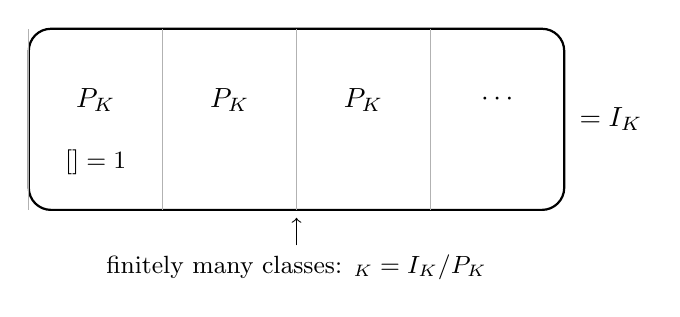
\begin{tikzpicture}[scale=1]
		\draw[rounded corners=8pt, thick] (-3.4,-1.15) rectangle (3.4,1.15);
		\foreach \x in {-2.55,-0.85,0.85,2.55}{
			\draw[gray!60] (\x-0.85,-1.15) -- (\x-0.85,1.15);
		}
		\node at (-2.55,0.25) {$P_K$};
		\node at (-0.85,0.25) {$\fa P_K$};
		\node at (0.85,0.25) {$\fb P_K$};
		\node at (2.55,0.25) {$\cdots$};
		\node at (-2.55,-0.55) {\small $[\fa]=1$};
		\node[right=2pt] at (3.4,0) {$= I_K$};
		\draw[->] (0,-1.6) -- (0,-1.25);
		\node[below] at (0,-1.6) {\small finitely many classes: $\Cl_K = I_K/P_K$};
	\end{tikzpicture}
\end{center}

The class group measures precisely the failure of unique factorisation.

\begin{theorem}\label{thm:pidufd}
	For a number field $K$ the following are equivalent:
	\begin{enumerate}[label=(\roman*)]
		\item $\OO_K$ is a principal ideal domain;
		\item $\OO_K$ is a unique factorisation domain;
		\item $\Cl_K$ is trivial.
	\end{enumerate}
\end{theorem}

\begin{proof}
	(i) $\iff$ (iii) is the definition, and (i) $\Rightarrow$ (ii) is a general fact from IB Groups, Rings and Modules.

	For (ii) $\Rightarrow$ (i), let $\fp$ be a nonzero prime ideal and pick $0 \neq x \in \fp$. Factor $x = \alpha_1\cdots\alpha_r$ into irreducibles. Since $\fp$ is prime, some $\alpha_i \in \fp$, so $(\alpha_i) \subseteq \fp$. In a UFD irreducibles are prime, so $(\alpha_i)$ is a nonzero prime ideal, hence maximal by Proposition \ref{prop:dedekind}(iv); as $\fp \neq \OO_K$ we get $(\alpha_i) = \fp$. So every prime ideal is principal, and by Theorem \ref{thm:uniquefac} every ideal is a product of primes, hence principal.
\end{proof}

\begin{remark}
	This is a genuinely useful equivalence, and not one that holds in general rings: an arbitrary UFD need not be a PID ($\Z[x]$, say). What makes it work is Dedekind-ness, specifically that nonzero primes are maximal.
\end{remark}

\begin{example}\label{ex:clsqrt5}
	In $\Z[\sqrt{-5}]$, the ideal $\fp = (2,1+\sqrt{-5})$ is not principal: if $\fp = (\beta)$ then $\fp^2 = (2)$ would give $\beta^2 = 2u$ for a unit $u = \pm1$, so $\Nm(\beta)^2 = 4$ and $\Nm(\beta) = 2$; but $a^2+5b^2 = 2$ is insoluble. So $[\fp] \neq 1$ while $[\fp]^2 = [(2)] = 1$, and $\Cl_{\Q(\sqrt{-5})}$ contains an element of order $2$. We will see in Section \ref{sec:computing} that in fact $\Cl_{\Q(\sqrt{-5})} \cong \Z/2\Z$.
\end{example}

\begin{example}\label{ex:conjinverse}
	Here is a useful trick in quadratic fields. Let $K = \Q(\sqrt d)$ and write $\bar{\cdot}$ for the nontrivial automorphism. For an ideal $\fa$, the conjugate $\bar\fa = \{\bar\alpha : \alpha \in \fa\}$ is again an ideal, and $[\bar\fa] = [\fa]^{-1}$, because $\fa\bar\fa$ is always principal. Indeed one can always write $\fa = (b, \alpha)$ with $b \in \Z$, and then
	$$\fa\bar\fa = \left(b^2,\, b\alpha,\, b\bar\alpha,\, \alpha\bar\alpha\right) = \left(b^2,\, b\alpha,\, b\Tr(\alpha),\, \Nm(\alpha)\right) = (b\alpha,\, c),$$
	where $c = \gcd\!\left(b^2,\, b\Tr(\alpha),\, \Nm(\alpha)\right)$,
	using $b\bar\alpha = b\Tr(\alpha) - b\alpha$. Now $x = b\alpha/c$ has $\Tr(x) = b\Tr(\alpha)/c \in \Z$ and $\Nm(x) = (b^2/c)(\Nm(\alpha)/c) \in \Z$, so $x \in \OO_K$ and $c \mid b\alpha$. Hence $\fa\bar\fa = (c)$ is principal. In particular, in Example \ref{ex:pcalc}, $\fq_2 = \bar{\fq_1}$ and indeed $[\fq_2] = [\fq_1]^{-1}$.
\end{example}

\subsection{The Norm of an Ideal}

We now attach a positive integer to each ideal, generalising $\abs{\Nm(\alpha)}$.

\begin{definition}[Ideal Norm]
	Let $\fa \trianglelefteq \OO_K$ be a nonzero ideal. Its \vocab{norm} is
	$$\Nm(\fa) = \abs{\OO_K/\fa} = [\OO_K : \fa],$$
	which is finite by Lemma \ref{lem:finitequot}.
\end{definition}

By Lagrange's theorem $\Nm(\fa)\cdot 1 = 0$ in $\OO_K/\fa$, so $\Nm(\fa) \in \fa \cap \Z$; equivalently $\fa \mid (\Nm(\fa))$.

\begin{example}
	For $p$ a rational prime and $n = [K:\Q]$, we have $\OO_K/(p) \cong (\Z/p\Z)^n$, so $\Nm((p)) = p^n$. More generally $\Nm((m)) = \abs{m}^n$ for $0 \neq m \in \Z$.
\end{example}

The essential property is multiplicativity, which is what makes the norm a useful bookkeeping device.

\begin{proposition}[Multiplicativity of the Norm]\label{prop:normmult}
	Let $\fa, \fb \trianglelefteq \OO_K$ be nonzero ideals. Then $\Nm(\fa\fb) = \Nm(\fa)\Nm(\fb)$.
\end{proposition}

\begin{proof}
	By unique factorisation and induction it suffices to treat $\fb = \fp$ prime. From the tower $\fa\fp \subseteq \fa \subseteq \OO_K$ and the third isomorphism theorem,
	$$\Nm(\fa\fp) = [\OO_K : \fa\fp] = [\OO_K:\fa]\,[\fa : \fa\fp] = \Nm(\fa)\,\abs{\fa/\fa\fp},$$
	so it suffices to show $\abs{\fa/\fa\fp} = \Nm(\fp)$.

	By unique factorisation $\fa \neq \fa\fp$, so choose $\alpha \in \fa \setminus \fa\fp$. We claim the map of abelian groups
	$$\phi : \OO_K/\fp \to \fa/\fa\fp, \qquad x + \fp \mapsto \alpha x + \fa\fp$$
	is a well-defined isomorphism; this gives the result. It is well defined since $\alpha\fp \subseteq \fa\fp$.

	\emph{Injectivity.} Since $(\alpha) \subseteq \fa$, Corollary \ref{cor:containdivide} gives $(\alpha) = \fa\fc$ for some ideal $\fc$. Suppose $\alpha x \in \fa\fp$. Then $x\fa\fc = x(\alpha) \subseteq \fa\fp$, so multiplying by $\fa^{-1}$, $x\fc \subseteq \fp$. As $\fp$ is prime, either $x \in \fp$ or $\fc \subseteq \fp$. But $\fc \subseteq \fp$ would give $(\alpha) = \fa\fc \subseteq \fa\fp$, contradicting the choice of $\alpha$. So $x \in \fp$, and $\phi$ is injective.

	\emph{Surjectivity.} We must show $(\alpha) + \fa\fp = \fa$. We know $\fa\fp \subsetneq (\alpha)+\fa\fp \subseteq \fa$, and multiplying by $\fa^{-1}$ gives
	$$\fp \subsetneq \left((\alpha)+\fa\fp\right)\fa^{-1} \subseteq \OO_K.$$
	Since $\fp$ is maximal, the middle term is $\OO_K$, so $(\alpha)+\fa\fp = \fa$ as required.
\end{proof}

\begin{remark}
	The conceptual proof runs as follows. By the Chinese remainder theorem $\OO_K/\prod\fp_i^{a_i} \cong \prod \OO_K/\fp_i^{a_i}$, so we reduce to prime powers; and then
	$$\abs{\OO_K/\fp^e} = \abs{\OO_K/\fp}\cdot\abs{\fp/\fp^2}\cdots\abs{\fp^{e-1}/\fp^e} = \Nm(\fp)^e,$$
	because each $\fp^i/\fp^{i+1}$ is a $1$-dimensional vector space over the field $\OO_K/\fp$ (it is nonzero by unique factorisation, and any $x \in \fp^i \setminus \fp^{i+1}$ generates, since $(x)+\fp^{i+1} = \fp^i$ by the maximality argument above). This last point is special to Dedekind domains: in $\F_p[x,y]$ with $\fp = (x,y)$ the quotient $\fp/\fp^2$ is $2$-dimensional. The proof we gave packages both steps at once.
\end{remark}

The norm of an ideal and the norm of an element agree where they should.

\begin{lemma}\label{lem:normprincipal}
	Let $0 \neq \alpha \in \OO_K$. Then $\Nm((\alpha)) = \abs{\Nm_{K/\Q}(\alpha)}$.
\end{lemma}

\begin{proof}
	Let $\gamma_1, \dots, \gamma_n$ be an integral basis of $\OO_K$; then $\alpha\gamma_1, \dots, \alpha\gamma_n$ is a $\Z$-basis of $(\alpha)$. Using Proposition \ref{prop:traceform},
	\begin{align*}
		\Delta(\alpha\gamma_1,\dots,\alpha\gamma_n) &= \det\left(\sigma_i(\alpha\gamma_j)\right)^2 = \det\left(\sigma_i(\alpha)\sigma_i(\gamma_j)\right)^2\\
		&= \left(\prod_i\sigma_i(\alpha)\right)^2\det(\sigma_i(\gamma_j))^2 = \Nm_{K/\Q}(\alpha)^2\, d_K.
	\end{align*}
	On the other hand, by Lemma \ref{lem:discindex} applied to the $\Z$-basis $\alpha\gamma_i$ of $(\alpha)$,
	$$\Delta(\alpha\gamma_1,\dots,\alpha\gamma_n) = [\OO_K : (\alpha)]^2 d_K = \Nm((\alpha))^2 d_K.$$
	Comparing and taking positive square roots gives the result.
\end{proof}

More generally the same computation identifies the discriminant of any ideal.

\begin{lemma}\label{lem:idealdisc}
	Let $\fa \trianglelefteq \OO_K$ be a nonzero ideal and let $\alpha_1, \dots, \alpha_n$ be a $\Z$-basis of $\fa$ (which exists by Lemma \ref{lem:finitequot}). Then the $\alpha_i$ form a $\Q$-basis of $K$ and
	$$\Delta(\alpha_1, \dots, \alpha_n) = \Nm(\fa)^2\, d_K.$$
\end{lemma}

\begin{proof}
	This is exactly Lemma \ref{lem:discindex} with $M = \fa$, once we note that $[\OO_K:\fa] = \Nm(\fa)$ and that a $\Z$-basis of $\fa$ is a $\Q$-basis of $K$ (since $\fa \supseteq m\OO_K$ for some $m \neq 0$, and $\fa$ has rank $n$).
\end{proof}

We record two consequences that we shall use constantly.

\begin{corollary}\label{cor:normbounds}
	Let $K$ be a number field.
	\begin{enumerate}[label=(\roman*)]
		\item For each $m \geq 1$ there are only finitely many ideals $\fa \trianglelefteq \OO_K$ with $\Nm(\fa) = m$.
		\item If $\Nm(\fa)$ is prime then $\fa$ is a prime ideal.
		\item If $\fa \subseteq \fb$ and $\Nm(\fa) = \Nm(\fb)$ then $\fa = \fb$.
	\end{enumerate}
\end{corollary}

\begin{proof}
	(i) If $\Nm(\fa) = m$ then $m \in \fa$, so $\fa \mid (m)$; and $(m)$ has only finitely many divisors by unique factorisation. (Alternatively: such $\fa$ correspond to ideals of the finite ring $\OO_K/m\OO_K$.)

	(ii) $\OO_K/\fa$ has prime order, so is $\Z/p\Z$, a field; hence $\fa$ is maximal, so prime.

	(iii) By Corollary \ref{cor:containdivide}, $\fa = \fb\fc$ for some ideal $\fc$, and taking norms $\Nm(\fc) = 1$, so $\fc = \OO_K$.
\end{proof}

\section{Factorisation of Primes}\label{sec:ram}

Unique factorisation of ideals reduces all questions about ideals to questions about prime ideals, so we had better understand what the prime ideals of $\OO_K$ look like. It turns out that they all sit above rational primes, and that finding them amounts to factoring polynomials mod $p$.

\subsection{Primes Above $p$}

\begin{lemma}\label{lem:primeabovep}
	Let $\fp \trianglelefteq \OO_K$ be a nonzero prime ideal. Then there is a unique rational prime $p$ with $\fp \mid (p)$, namely the one with $\fp \cap \Z = p\Z$. Moreover $\Nm(\fp) = p^f$ for some $1 \leq f \leq n = [K:\Q]$.
\end{lemma}

\begin{proof}
	$\fp \cap \Z$ is an ideal of $\Z$, hence $= m\Z$ for some $m \geq 0$, and $m \neq 0$ by Lemma \ref{lem:finitequot}. If $m = ab$ with $a,b \in \Z$, then $ab \in \fp$ so $a \in \fp$ or $b \in \fp$, giving $m \mid a$ or $m \mid b$; hence $m = p$ is prime. Then $p \in \fp$, so $(p) \subseteq \fp$ and $\fp \mid (p)$ by Corollary \ref{cor:containdivide}. Uniqueness is clear since $\fp \cap \Z$ determines $p$, and if $\fp \mid (q)$ for a prime $q \neq p$ then $q \in \fp\cap\Z = p\Z$, absurd.

	Writing $(p) = \fp\fa$ and taking norms, $p^n = \Nm(\fp)\Nm(\fa)$, so $\Nm(\fp) = p^f$ with $1 \le f \le n$ (note $\Nm(\fp) > 1$ as $\fp \neq \OO_K$).
\end{proof}

So to find all the prime ideals of $\OO_K$, it is enough to factorise $(p)$ for each rational prime $p$. This motivates the following language.

\begin{definition}[Ramification Index and Residue Degree]
	Let $p$ be a rational prime and let
	$$p\OO_K = \fp_1^{e_1}\cdots\fp_g^{e_g}$$
	be its factorisation into distinct primes. We say $\fp_i$ \vocab{lies above} $p$, written $\fp_i \mid p$. The integer $e_i$ is the \vocab{ramification index} of $\fp_i$ over $p$, and $f_i$ defined by $\Nm(\fp_i) = p^{f_i}$ is the \vocab{residue degree}. Equivalently $f_i = [\OO_K/\fp_i : \F_p]$, since $\OO_K/\fp_i$ is a finite field containing $\F_p = \Z/p\Z$.
\end{definition}

\begin{theorem}[The Fundamental Identity]\label{thm:efg}
	With the notation above, $\displaystyle\sum_{i=1}^g e_if_i = n = [K:\Q]$.
\end{theorem}

\begin{proof}
	Take norms in $p\OO_K = \prod_i\fp_i^{e_i}$ and use Proposition \ref{prop:normmult}:
	$$p^n = \Nm((p)) = \prod_i\Nm(\fp_i)^{e_i} = p^{\sum_i e_if_i}. \qedhere$$
\end{proof}

The picture to have in mind is a tower, with $p$ at the bottom in $\Z$ and the primes above it in $\OO_K$, each labelled with its $e$ and $f$.

\begin{center}
	\begin{tikzpicture}[scale=1, every node/.style={font=\small}]
		\node (Z) at (-4.6,0) {$\Z$};
		\node (O) at (-4.6,2.0) {$\OO_K$};
		\draw[right hook->] (Z) -- (O);
		\node (p) at (0,0) {$p\Z$};
		\node (p1) at (-2.4,2.0) {$\fp_1$};
		\node (p2) at (-0.8,2.0) {$\fp_2$};
		\node (dots) at (0.8,2.0) {$\cdots$};
		\node (pg) at (2.4,2.0) {$\fp_g$};
		\draw (p) -- (p1); \draw (p) -- (p2); \draw (p) -- (dots); \draw (p) -- (pg);
		\node[above=3pt, font=\scriptsize] at (p1) {$(e_1,f_1)$};
		\node[above=3pt, font=\scriptsize] at (p2) {$(e_2,f_2)$};
		\node[above=3pt, font=\scriptsize] at (pg) {$(e_g,f_g)$};
		\node at (0,-0.9) {$e_1f_1 + e_2f_2 + \dots + e_gf_g = n$};
	\end{tikzpicture}
\end{center}

\begin{definition}[Split, Inert, Ramified]
	Let $p$ be a rational prime and $p\OO_K = \prod_i\fp_i^{e_i}$ as above. We say $p$ is
	\begin{itemize}
		\item \vocab{ramified} in $K$ if $e_i > 1$ for some $i$, and \vocab{unramified} otherwise;
		\item \vocab{inert} in $K$ if $g = 1$ and $e_1 = 1$, so that $(p)$ stays prime;
		\item \vocab{totally split} (or \vocab{split completely}) if $g = n$, so that $e_i = f_i = 1$ for all $i$;
		\item \vocab{totally ramified} if $g = 1$ and $e_1 = n$.
	\end{itemize}
\end{definition}

We will see that only finitely many primes ramify, namely the divisors of $d_K$.

In the Galois case the picture is much more uniform, because the Galois group shuffles the primes above $p$ among themselves.

\begin{proposition}[Splitting in Galois Extensions]\label{prop:galoissplit}
	Let $K/\Q$ be Galois with group $G$, and let $p$ be a rational prime with $p\OO_K = \fp_1^{e_1}\cdots\fp_g^{e_g}$. Then $G$ acts transitively on $\{\fp_1,\dots,\fp_g\}$. Consequently $e_1 = \dots = e_g =: e$ and $f_1 = \dots = f_g =: f$, and
	$$efg = n = [K:\Q].$$
\end{proposition}

\begin{proof}
	First note that $G$ preserves $\OO_K$: if $\alpha$ satisfies a monic $h \in \Z[x]$ and $\tau \in G$, then $h(\tau\alpha) = \tau(h(\alpha)) = 0$, so $\tau\alpha \in \OO_K$. Hence $\tau$ permutes the ideals of $\OO_K$, preserving primality and fixing $(p)$, so it permutes $\{\fp_1,\dots,\fp_g\}$.

	Suppose the action is not transitive, so some $\fq = \fp_j$ is not of the form $\tau(\fp_1)$ for any $\tau$. By the Chinese remainder theorem (the $\tau(\fp_1)$ and $\fq$ being distinct maximal ideals) pick $x \in \OO_K$ with
	$$x \equiv 0 \pmod{\fq}, \qquad x \equiv 1 \pmod{\tau(\fp_1)} \text{ for all } \tau \in G.$$
	Then $\Nm_{K/\Q}(x) = \prod_{\tau\in G}\tau(x) \in \fq \cap \Z = p\Z \subseteq \fp_1$, so some $\tau(x) \in \fp_1$, i.e.\ $x \in \tau^{-1}(\fp_1)$ -- contradicting $x \equiv 1$ there.

	Finally, applying $\tau$ to the factorisation of $(p)$ permutes the $\fp_i$ while fixing $(p)$, so by uniqueness the exponents match up: $e_i = e_j$ whenever $\tau(\fp_i) = \fp_j$. And $\tau$ induces an isomorphism $\OO_K/\fp_i \to \OO_K/\tau(\fp_i)$, so the $f_i$ agree too. Transitivity then makes all $e_i$ and all $f_i$ equal, and Theorem \ref{thm:efg} becomes $efg = n$.
\end{proof}

\begin{example}
	In $\Q(i)$, $n = 2$, so $(e,f,g)$ is $(1,1,2)$ for split primes, $(1,2,1)$ for inert primes and $(2,1,1)$ for the ramified prime $2$ -- exactly the trichotomy of Proposition \ref{prop:quadsplit}. In $\Q(\zeta_7)$, $n=6$, and the possible unramified behaviours are $(1,f,6/f)$ for $f \mid 6$. Contrast this with $\Q(\sqrt[3]2)$, which is \emph{not} Galois: there we found $(5) = \fp_1\fp_2$ with $f_1 = 1$ and $f_2 = 2$, which is impossible in a Galois extension.
\end{example}

\subsection{Dedekind's Criterion}

Suppose we can write $\OO_K = \Z[\alpha]$ for some $\alpha$ with minimal polynomial $g \in \Z[x]$. Then
$$\OO_K/p\OO_K \cong \Z[x]/(g(x), p) \cong \F_p[x]/(\bar g(x)),$$
and the ideals of $\OO_K$ containing $p$ correspond to the ideals of this ring, which correspond in turn to the monic factors of $\bar g$ in $\F_p[x]$. So factoring $(p)$ becomes factoring a polynomial mod $p$ -- a completely mechanical task. Remarkably, this works even when $\Z[\alpha] \neq \OO_K$, provided $p$ does not divide the index.

\begin{theorem}[Dedekind's Criterion]\label{thm:dedekindcrit}
	Let $K$ be a number field, let $\alpha \in \OO_K$ with $K = \Q(\alpha)$ and minimal polynomial $g \in \Z[x]$, and let $p$ be a prime with $p \nmid [\OO_K : \Z[\alpha]]$. Let
	$$\bar g = \bar\varphi_1^{\,e_1}\cdots\bar\varphi_g^{\,e_g}$$
	be the factorisation of $\bar g = g \bmod p$ into distinct monic irreducibles in $\F_p[x]$, and lift each $\bar\varphi_i$ to a monic $\varphi_i \in \Z[x]$ of the same degree. Then
	$$p\OO_K = \fp_1^{e_1}\cdots\fp_g^{e_g}, \qquad \fp_i = \left(p, \varphi_i(\alpha)\right),$$
	the $\fp_i$ are distinct primes, and $\Nm(\fp_i) = p^{f_i}$ with $f_i = \deg\bar\varphi_i$.
\end{theorem}

\begin{proof}
	\emph{Step 1: the ideals $\fq_i = (p,\varphi_i(\alpha)) \trianglelefteq \Z[\alpha]$ are prime with $\Z[\alpha]/\fq_i \cong \F_p[x]/(\bar\varphi_i)$.} Consider the surjective ring homomorphism $\Z[x] \to \F_p[x]/(\bar\varphi_i)$ given by reduction mod $p$ followed by reduction mod $\bar\varphi_i$. Its kernel contains $p$ and $\varphi_i$; conversely, if $f$ maps to zero then $\bar\varphi_i \mid \bar f$, so $\bar f = \bar\varphi_i\bar h$ for some $\bar h$, and lifting $\bar h$ to $h \in \Z[x]$ gives $f - \varphi_i h \in p\Z[x]$. So the kernel is exactly $(p, \varphi_i)$. Since $g(\alpha) = 0$ and $\bar\varphi_i \mid \bar g$, the map factors through $\Z[x]/(g) \cong \Z[\alpha]$, and the same argument shows that the induced map $\Z[\alpha] \to \F_p[x]/(\bar\varphi_i)$ has kernel $\fq_i = (p,\varphi_i(\alpha))$. As $\bar\varphi_i$ is irreducible, $\F_p[x]/(\bar\varphi_i) \cong \F_{p^{f_i}}$ is a field, so $\fq_i$ is prime with $\abs{\Z[\alpha]/\fq_i} = p^{f_i}$.

	\emph{Step 2: $\iota : \Z[\alpha]/p\Z[\alpha] \to \OO_K/p\OO_K$ is an isomorphism.} Write $M = \OO_K/\Z[\alpha]$, a finite abelian group of order coprime to $p$ by hypothesis. Multiplication by $p$ on $M$ is injective (its kernel is a $p$-group inside a group of order prime to $p$), hence bijective as $M$ is finite. Now the kernel of $\iota$ is $(\Z[\alpha]\cap p\OO_K)/p\Z[\alpha]$, and an element of this is $x \in \Z[\alpha]$ with $x = py$, $y \in \OO_K$; then $py \equiv 0$ in $M$, so $y \in \Z[\alpha]$ and $x \in p\Z[\alpha]$. So $\iota$ is injective. For surjectivity we need $\OO_K = \Z[\alpha] + p\OO_K$, i.e.\ $pM = M$, which is the surjectivity of multiplication by $p$ on $M$. Comparing orders, $\iota$ is an isomorphism.

	\emph{Step 3.} By Step 2, ideals of $\OO_K$ containing $p$ correspond to ideals of $\Z[\alpha]$ containing $p$, with $\fq \mapsto \fq\OO_K$ and $\fp \mapsto \fp\cap\Z[\alpha]$, and the quotients agree. So each $\fp_i := \fq_i\OO_K = (p, \varphi_i(\alpha))$ is a prime ideal of $\OO_K$ with $\Nm(\fp_i) = p^{f_i}$, and $\fp_i \neq \fp_j$ for $i \neq j$ since $\bar\varphi_i, \bar\varphi_j$ are coprime, whence $\fq_i + \fq_j = \Z[\alpha]$.

	\emph{Step 4: the factorisation.} Since $(p,\varphi_i(\alpha))^{e_i} \subseteq (p, \varphi_i(\alpha)^{e_i})$, we get
	$$\fp_1^{e_1}\cdots\fp_g^{e_g} \subseteq \left(p,\ \varphi_1(\alpha)^{e_1}\cdots\varphi_g(\alpha)^{e_g}\right).$$
	Now $\overline{\varphi_1^{e_1}\cdots\varphi_g^{e_g}} = \bar g$, so $\varphi_1^{e_1}\cdots\varphi_g^{e_g} = g + ps$ for some $s \in \Z[x]$, and evaluating at $\alpha$ (where $g(\alpha) = 0$) shows the right-hand ideal is $(p, ps(\alpha)) = (p)$. So $\prod_i\fp_i^{e_i} \subseteq (p)$. But $\deg g = n$ gives $\sum_i e_if_i = n$, so
	$$\Nm\left(\prod_i\fp_i^{e_i}\right) = p^{\sum_ie_if_i} = p^n = \Nm((p)),$$
	and Corollary \ref{cor:normbounds}(iii) forces equality.
\end{proof}

\begin{remark}
	The hypothesis $p \nmid [\OO_K:\Z[\alpha]]$ is essential but mild in practice: for any fixed $\alpha$ generating $K$ with $\alpha\in\OO_K$, only finitely many primes divide the index, so Dedekind's criterion factors $(p)$ for all but finitely many $p$. Different lifts $\varphi_i$ give the same ideal, since they differ by a multiple of $p \in \fp_i$.
\end{remark}

\begin{example}\label{ex:cbrt2}
	Let $K = \Q(\sqrt[3]2)$, so $\OO_K = \Z[\sqrt[3]2]$ and $g = x^3-2$; the index is $1$, so Dedekind applies to every $p$.
	\begin{enumerate}[label=(\roman*)]
		\item $p = 2$: $\bar g = x^3$, so $(2) = \fp^3$ with $\fp = (2, \sqrt[3]2) = (\sqrt[3]2)$. So $2$ is totally ramified, with $e = 3, f = 1$.
		\item $p = 3$: $\bar g = x^3 - 2 = x^3+1 = (x+1)^3$ in $\F_3[x]$, so $(3) = (3, 1+\sqrt[3]2)^3$; again totally ramified.
		\item $p = 5$: $2$ is a cube mod $5$ (namely $3^3 = 27 \equiv 2$), and $x^3-2 = (x-3)(x^2+3x+4)$ in $\F_5[x]$, the quadratic factor being irreducible as its discriminant $9-16 = -7 \equiv 3$ is not a square mod $5$. So
		$$(5) = \left(5, \sqrt[3]2 - 3\right)\left(5, \sqrt[3]4 + 3\sqrt[3]2+4\right),$$
		with $(e,f) = (1,1)$ and $(1,2)$; indeed $1\cdot1 + 1\cdot 2 = 3$.
		\item $p = 7$: the cubes mod $7$ are $\{0,1,6\}$, so $x^3-2$ has no root mod $7$; being cubic it is irreducible, and $7$ is inert with $f = 3$.
		\item $p = 31$: here $x^3 - 2 \equiv (x-4)(x-7)(x-20)$, so $31$ is totally split.
	\end{enumerate}
	Notice that $2$ and $3$ ramify, and $d_K = -108 = -2^2\cdot 3^3$. This is not a coincidence.
\end{example}

\begin{example}[A Non-Monogenic Field]\label{ex:nonmonogenic}
	Return to $K = \Q(\alpha)$ with $\alpha^3-\alpha^2-2\alpha-8 = 0$, where $d_K = -503$ and $[\OO_K:\Z[\alpha]] = 2$ (Example \ref{ex:cubicdisc}). Dedekind's criterion does \emph{not} apply at $p=2$; and indeed $\bar g = x^2(x+1)$ in $\F_2[x]$ would predict $(2) = \fp^2\fq$, which is wrong. In fact $2$ splits completely, $(2) = \fp_1\fp_2\fp_3$ with all $e_i = f_i = 1$ (one checks this using the integral basis $1, \alpha, \beta$).

	This has a striking consequence: for \emph{every} $\gamma \in \OO_K \setminus \Z$, the index $[\OO_K:\Z[\gamma]]$ is even, so $\OO_K \neq \Z[\gamma]$. Indeed, if $2 \nmid [\OO_K:\Z[\gamma]]$ then Dedekind's criterion would say that the minimal polynomial of $\gamma$ has three distinct roots in $\F_2$ -- but $\F_2$ only has two elements. So $K$ has no integral basis of the form $1,\gamma,\gamma^2$: it is not \vocab{monogenic}. The same argument gives a general obstruction.
\end{example}

\begin{corollary}
	Let $p < n = [K:\Q]$ be a prime and suppose $\OO_K = \Z[\alpha]$ for some $\alpha$. Then $p$ does not split completely in $K$.
\end{corollary}

\begin{proof}
	If $p$ split completely then, by Dedekind's criterion, the minimal polynomial of $\alpha$ would have $n$ distinct roots in $\F_p$; but $\abs{\F_p} = p < n$.
\end{proof}

\subsection{Primes in Quadratic Fields}

The quadratic case is worth doing completely, because it is where we shall do most of our computations, and because the answer is a beautiful reformulation of quadratic reciprocity.

\begin{proposition}\label{prop:quadsplit}
	Let $K = \Q(\sqrt d)$ with $d$ squarefree, and let $p$ be an odd prime. Then
	$$p\OO_K = \begin{cases}
		\fp_1\fp_2 \text{ with } \fp_1 \neq \fp_2 & \text{if } \legendre{d}{p} = 1 \quad (\text{$p$ splits}),\\
		\fp \text{ prime} & \text{if } \legendre{d}{p} = -1 \quad (\text{$p$ inert}),\\
		\fp^2 & \text{if } p \mid d \quad (\text{$p$ ramifies}),
	\end{cases}$$
	where $\legendre{\cdot}{p}$ is the Legendre symbol. Explicitly, if $r^2 \equiv d \pmod p$ then $\fp_{1,2} = (p, \sqrt d \mp r)$, and in the ramified case $\fp = (p,\sqrt d)$.
\end{proposition}

\begin{proof}
	Whether $d \equiv 1 \pmod 4$ or not, $\Z[\sqrt d] \subseteq \OO_K$ has index $1$ or $2$, which is coprime to the odd prime $p$. So Dedekind's criterion applies with $\alpha = \sqrt d$, $g = x^2-d$, and we simply factor $x^2 - d$ in $\F_p[x]$: it has two distinct roots, no roots, or a repeated root according as $d$ is a nonzero square, a nonsquare, or zero mod $p$.
\end{proof}

The prime $2$ needs separate treatment, and here the $d \bmod 4$ dichotomy resurfaces.

\begin{lemma}\label{lem:p2quad}
	Let $K = \Q(\sqrt d)$ with $d$ squarefree. Then $2$ splits if $d \equiv 1 \pmod 8$, is inert if $d \equiv 5 \pmod 8$, and ramifies if $d \equiv 2,3\pmod 4$.
\end{lemma}

\begin{proof}
	If $d \equiv 1 \pmod 4$ then $\OO_K = \Z[\alpha]$ with $\alpha = \tfrac12(1+\sqrt d)$, whose minimal polynomial is $x^2 - x + \tfrac14(1-d)$; the index is $1$ so Dedekind applies. Modulo $2$ this is $x^2+x+c$ where $c = \tfrac14(1-d) \bmod 2$. If $d \equiv 1 \pmod 8$ then $c = 0$ and we get $x(x+1)$, so $2$ splits. If $d \equiv 5\pmod 8$ then $c = 1$ and $x^2+x+1$ is irreducible over $\F_2$, so $2$ is inert.

	If $d \equiv 2,3\pmod 4$ then $\OO_K = \Z[\sqrt d]$ and $x^2-d$ reduces mod $2$ to $x^2$ or $x^2+1 = (x+1)^2$, so $2$ ramifies.
\end{proof}

Comparing with Example \ref{ex:quaddisc} -- where $d_K = d$ if $d \equiv 1 \pmod 4$ and $4d$ otherwise -- gives a clean statement.

\begin{corollary}\label{cor:quadram}
	Let $K = \Q(\sqrt d)$ be a quadratic field. A prime $p$ ramifies in $K$ if and only if $p \mid d_K$.
\end{corollary}

\begin{proof}
	For odd $p$: $p$ ramifies iff $p \mid d$, and since $d_K \in \{d,4d\}$ this holds iff $p \mid d_K$. For $p = 2$: by Lemma \ref{lem:p2quad}, $2$ ramifies iff $d \equiv 2,3\pmod 4$, which is exactly when $d_K = 4d$ is even; and if $d \equiv 1\pmod 4$ then $d_K = d$ is odd.
\end{proof}

Here are the three behaviours side by side, drawn as towers.

\begin{center}
	\begin{tikzpicture}[scale=0.95, every node/.style={font=\small}]
		% split
		\begin{scope}[xshift=0cm]
			\node (b) at (0,0) {$p$};
			\node (l) at (-0.7,1.3) {$\fp_1$};
			\node (r) at (0.7,1.3) {$\fp_2$};
			\draw (b) -- (l); \draw (b) -- (r);
			\node at (0,-0.75) {split};
			\node at (0,-1.3) {\scriptsize $e=f=1,\ g=2$};
		\end{scope}
		% inert
		\begin{scope}[xshift=4.2cm]
			\node (b2) at (0,0) {$p$};
			\node (t2) at (0,1.3) {$\fp$};
			\draw (b2) -- node[right=1pt,font=\scriptsize] {$f=2$} (t2);
			\node at (0,-0.75) {inert};
			\node at (0,-1.3) {\scriptsize $e=1,\ f=2,\ g=1$};
		\end{scope}
		% ramified
		\begin{scope}[xshift=8.4cm]
			\node (b3) at (0,0) {$p$};
			\node (t3) at (0,1.3) {$\fp$};
			\draw (-0.055,0.28) -- (-0.055,1.02);
			\draw (0.055,0.28) -- (0.055,1.02);
			\node[right=3pt,font=\scriptsize] at (0.055,0.65) {$e=2$};
			\node at (0,-0.75) {ramified};
			\node at (0,-1.3) {\scriptsize $e=2,\ f=1,\ g=1$};
		\end{scope}
	\end{tikzpicture}
\end{center}

\begin{example}\label{ex:quadfactor}
	Let $K = \Q(\sqrt{-5})$, so $d_K = -20$.
	\begin{itemize}
		\item $p=2$: $-5 \equiv 3 \pmod 4$, so $2$ ramifies: $(2) = (2,1+\sqrt{-5})^2$, as we computed directly in Example \ref{ex:pcalc}.
		\item $p=3$: $x^2+5 \equiv x^2-1 = (x-1)(x+1) \pmod 3$, so $(3) = (3,\sqrt{-5}-1)(3,\sqrt{-5}+1)$.
		\item $p=5$: $5 \mid d_K$, so $5$ ramifies: $(5) = (\sqrt{-5})^2$.
		\item $p=7$: the squares mod $7$ are $1,2,4$, and $-5 \equiv 2$, so $7$ splits: indeed $x^2+5 \equiv (x-3)(x+3) \pmod 7$.
		\item $p=11$: $-5 \equiv 6 \pmod{11}$, and $6$ is not a square mod $11$, so $11$ is inert.
	\end{itemize}
	This confirms in particular that the ideals $\fp, \fq_1, \fq_2$ of Example \ref{ex:pcalc} really are prime.
\end{example}

\begin{example}
	Let $K = \Q(\sqrt{-11})$, so $-11 \equiv 1 \pmod 4$ and $\OO_K = \Z[\tfrac12(1+\sqrt{-11})]$, in which $\Z[\sqrt{-11}]$ has index $2$. To factor $(5)$ we may use $\alpha = \sqrt{-11}$, since $5 \nmid 2$: modulo $5$ we have $x^2+11 \equiv x^2+1 = (x-2)(x+2)$, so
	$$(5) = \left(5, \sqrt{-11}-2\right)\left(5,\sqrt{-11}+2\right).$$
\end{example}

\subsection{Ramification and the Discriminant}

Corollary \ref{cor:quadram} is a special case of a general and important theorem.

\begin{theorem}[Ramification and the Discriminant]\label{thm:ramdisc}
	Let $K$ be a number field and $p$ a rational prime. Then $p$ ramifies in $K$ if and only if $p \mid d_K$. In particular only finitely many primes ramify.
\end{theorem}

We shall not give the full proof, but the idea in the direction we use most is clear from Dedekind's criterion: if $\OO_K = \Z[\alpha]$ with minimal polynomial $g$, then $p$ ramifies exactly when $\bar g$ has a repeated factor in $\F_p[x]$, which happens exactly when $\disc(\bar g) = 0$ in $\F_p$, i.e.\ when $p \mid \disc(g) = d_K$. The general case is handled by reducing to this one after localising.

\begin{example}
	In Example \ref{ex:cbrt2} we found that exactly $2$ and $3$ ramify in $\Q(\sqrt[3]2)$, and $d_K = -108 = -2^2 3^3$. In Example \ref{ex:nonmonogenic}, $d_K = -503$ is prime, so $503$ is the only ramified prime; in particular $2$ is unramified, consistent with $(2) = \fp_1\fp_2\fp_3$.
\end{example}

The theorem has a famous consequence, once we know (Section \ref{sec:geom}) that $\abs{d_K} > 1$ whenever $K \neq \Q$: \emph{every number field other than $\Q$ has at least one ramified prime}. Equivalently, $\Q$ admits no unramified extensions. This is the arithmetic analogue of the fact that the sphere is simply connected.

\subsection{Cyclotomic Fields}\label{sec:cyclo}

We finish the section with the other family of number fields that everyone should know. Let $\zeta = \zeta_m = e^{2\pi i/m}$ and $K = \Q(\zeta_m)$, the $m$th \vocab{cyclotomic field}.

\begin{proposition}\label{prop:cyclo}
	Let $K = \Q(\zeta_m)$. Then
	\begin{enumerate}[label=(\roman*)]
		\item $[K:\Q] = \varphi(m)$, and $K/\Q$ is Galois with $\Gal(K/\Q) \cong (\Z/m\Z)^\times$, the class of $r$ acting by $\zeta_m \mapsto \zeta_m^r$;
		\item $\OO_K = \Z[\zeta_m]$;
		\item a prime $p$ ramifies in $K$ if and only if $p \mid m$ (for $m \not\equiv 2 \bmod 4$);
		\item if $p \nmid m$, then $p\OO_K$ is a product of $\varphi(m)/f$ distinct primes each of residue degree $f$, where $f$ is the multiplicative order of $p$ modulo $m$. In particular $p$ splits completely if and only if $p \equiv 1 \pmod m$.
	\end{enumerate}
\end{proposition}

\begin{proof}
	Parts (i) is from Galois Theory: the minimal polynomial of $\zeta_m$ is the cyclotomic polynomial $\Phi_m$, of degree $\varphi(m)$. Part (ii) we take on trust in general (for $m = p$ prime it is a standard exercise, sketched below), and (iii) follows from (ii) and Theorem \ref{thm:ramdisc}.

	For (iv), assume $p \nmid m$; by (ii) and Theorem \ref{thm:dedekindcrit} we must factor $\Phi_m$ in $\F_p[x]$. Since $p\nmid m$, the polynomial $x^m - 1$ is separable mod $p$, so $\bar\Phi_m = \bar\gamma_1\cdots\bar\gamma_g$ with distinct irreducible factors $\bar\gamma_i$ (this re-proves that $p$ is unramified). The Galois group $G \cong (\Z/m\Z)^\times$ preserves $\OO_K$, hence acts on the set of primes above $p$, and acts transitively on the roots of $\Phi_m$; so it permutes the $\bar\gamma_i$ transitively and they all have the same degree $f'$, say, with $gf' = \varphi(m)$.

	It remains to show $f' = f = \operatorname{ord}_m(p)$. In $\F_p[x]/(\bar\gamma_1) \cong \F_{p^{f'}}$, the image of $x$ is the image of $\zeta_m$, which is a root of $x^m-1$ of exact order $m$ (as $x^m-1$ is separable mod $p$ and $\Phi_m \mid x^m-1$). So $m$ divides $\abs{\F_{p^{f'}}^\times} = p^{f'}-1$, giving $p^{f'} \equiv 1 \pmod m$ and hence $f \mid f'$. Conversely the Frobenius $\alpha\mapsto\alpha^p$ generates $\Gal(\F_{p^{f'}}/\F_p)$, and it acts on $\zeta_m$ as the element $p \in (\Z/m\Z)^\times$, which has order $f$; so $f' \mid f$. Hence $f = f'$.
\end{proof}

\begin{example}[The Prime Case]\label{ex:cyclop}
	Let $p$ be an odd prime and $K = \Q(\zeta_p)$, so $[K:\Q] = p-1$. Put $\lambda = 1-\zeta_p$. Since
	$$\Phi_p(x) = \frac{x^p-1}{x-1} = \prod_{k=1}^{p-1}\left(x - \zeta_p^k\right),$$
	setting $x = 1$ gives
	$$p = \Phi_p(1) = \prod_{k=1}^{p-1}\left(1-\zeta_p^k\right) = \Nm_{K/\Q}(\lambda).$$
	Moreover $(1-\zeta_p^k)/(1-\zeta_p) = 1 + \zeta_p + \dots+\zeta_p^{k-1} \in \Z[\zeta_p]$ is a unit for $1 \leq k \leq p-1$ (its inverse is $(1-\zeta_p)/(1-\zeta_p^k)$, of the same shape after writing $\zeta_p = (\zeta_p^k)^{k'}$ with $kk'\equiv 1$). Hence all the $1 - \zeta_p^k$ are associates and
	$$(p) = (\lambda)^{p-1}.$$
	So $p$ is totally ramified in $\Q(\zeta_p)$, with $e = p-1$, $f = g = 1$, and $\Nm((\lambda)) = p$, so $(\lambda)$ is prime.

	One deduces $\OO_K = \Z[\zeta_p]$ as follows. From $\disc(\Phi_p) = (-1)^{(p-1)/2}p^{\,p-2}$, the index $m = [\OO_K:\Z[\zeta_p]]$ satisfies $m^2 \mid p^{p-2}$, so $m$ is a power of $p$; and one checks using the totally ramified prime $\lambda$ that $p \nmid m$. Hence $m=1$ and $d_K = (-1)^{(p-1)/2}p^{p-2}$.
\end{example}

\begin{example}
	Take $m = 8$, so $\Phi_8(x) = x^4+1$ and $K = \Q(\zeta_8)$ has degree $4$ with $\Gal(K/\Q) \cong (\Z/8\Z)^\times \cong (\Z/2\Z)^2$. Then $2$ is totally ramified. For odd $p$, the order of $p$ mod $8$ is $1$ if $p \equiv 1$ and $2$ otherwise. So $p \equiv 1\pmod 8$ splits completely into four primes, and every other odd $p$ factors into two primes of residue degree $2$. For instance $x^4+1$ factors into four linear factors mod $17$, and into two irreducible quadratics mod $3$.
\end{example}

\begin{example}
	Take $m = 7$, so $K = \Q(\zeta_7)$ has degree $6$ and $\Gal(K/\Q)\cong(\Z/7\Z)^\times$ is cyclic of order $6$, generated by the class of $3$.
	\begin{itemize}
		\item $p = 7$ is totally ramified: $(7) = (1-\zeta_7)^6$, by Example \ref{ex:cyclop}.
		\item $p=2$: the powers of $2$ mod $7$ are $2,4,1$, so $f = 3$ and $(2) = \fp_1\fp_2$ with $\Nm(\fp_i) = 8$. Correspondingly $\Phi_7$ factors mod $2$ into two irreducible cubics, namely $(x^3+x+1)(x^3+x^2+1)$.
		\item $p=3$: the class of $3$ generates the whole group, so $f = 6$ and $3$ is inert; equivalently $\Phi_7$ is irreducible mod $3$.
		\item $p = 29 \equiv 1 \pmod 7$: here $f=1$, so $29$ splits completely into six primes of norm $29$.
	\end{itemize}
	In each case $\sum e_if_i = 6$, as it must.
\end{example}

\begin{remark}[Cyclotomic Fields and Reciprocity]
	Since $\Gal(\Q(\zeta_p)/\Q)$ is cyclic of order $p-1$, it has a unique subgroup of index $2$, so $\Q(\zeta_p)$ contains a unique quadratic subfield. Comparing discriminants (only $p$ ramifies, and the discriminant of $\Q(\sqrt d)$ must therefore be $\pm p$) shows that this subfield is
	$$\Q\left(\sqrt{p^*}\right), \qquad p^* = (-1)^{(p-1)/2}p.$$
	Now Proposition \ref{prop:cyclo}(iv) says that the splitting of $q$ in $\Q(\zeta_p)$ depends only on $q$ mod $p$; hence so does its splitting in the subfield $\Q(\sqrt{p^*})$, which by Proposition \ref{prop:quadsplit} is governed by $\legendre{p^*}{q}$. So $\legendre{p^*}{q}$ depends only on $q \bmod p$ -- and unwinding this is precisely the law of quadratic reciprocity. This is the first hint of \emph{class field theory}: abelian extensions of $\Q$ are exactly the subfields of cyclotomic fields, and splitting in them is governed by congruences.
\end{remark}

\section{The Geometry of Numbers}\label{sec:geom}

We now come to the geometric heart of the course. The idea is due to Minkowski, and it is disarmingly simple: realise $\OO_K$ as a lattice in a Euclidean space, and use the fact that a large enough convex body must contain a lattice point. From this one deduces that every ideal class contains an ideal of small norm, and hence that the class group is finite.

\subsection{Lattices}

\begin{definition}[Discrete]
	A subset $X \subseteq \R^n$ is \vocab{discrete} if $X \cap C$ is finite for every compact $C \subseteq \R^n$; equivalently, if every $x \in X$ has $\varepsilon > 0$ with $B_\varepsilon(x)\cap X = \{x\}$.
\end{definition}

\begin{proposition}\label{prop:discrete}
	Let $\Lambda \subseteq \R^n$ be a subgroup of $(\R^n,+)$. Then $\Lambda$ is discrete if and only if
	$$\Lambda = \Z x_1 \oplus \dots \oplus \Z x_m$$
	for some $x_1,\dots,x_m \in \R^n$ linearly independent over $\R$.
\end{proposition}

\begin{proof}
	($\Leftarrow$) Extend $x_1, \dots, x_m$ to a basis of $\R^n$ and let $g \in \GL_n(\R)$ take $x_i$ to the standard basis vector $e_i$. Discreteness is preserved by $g$, and $\bigoplus_{i\le m}\Z e_i$ is visibly discrete.

	($\Rightarrow$) Choose $y_1, \dots, y_m \in \Lambda$ that are $\R$-linearly independent with $m$ maximal, so $m \le n$, and let $V = \operatorname{span}_\R(y_1,\dots,y_m)$; by maximality $\Lambda \subseteq V$. Let
	$$X = \left\{\textstyle\sum_i \lambda_iy_i : \lambda_i \in [0,1]\right\},$$
	a compact set, so $X \cap \Lambda$ is finite. Put $\Lambda_0 = \bigoplus_i \Z y_i \subseteq \Lambda$. Any $\lambda \in \Lambda$ can be written as $\lambda = \lambda_0 + \lambda_1$ with $\lambda_0 \in \Lambda_0$ (the integer parts of the coordinates) and $\lambda_1 \in X \cap \Lambda$ (the fractional parts). Hence $[\Lambda : \Lambda_0] \le \abs{X\cap\Lambda} < \infty$.

	Let $D = [\Lambda:\Lambda_0]$. By Lagrange, $D\Lambda \subseteq \Lambda_0$, so
	$$\Lambda_0 \subseteq \Lambda \subseteq \tfrac{1}{D}\Lambda_0 \cong \Z^m.$$
	So $\Lambda$ is a subgroup of a free abelian group of rank $m$, hence free of rank at most $m$; and it contains $\Lambda_0$ of rank $m$, so has rank exactly $m$. A $\Z$-basis $x_1,\dots,x_m$ of $\Lambda$ then spans $V$ over $\R$, so is $\R$-linearly independent.
\end{proof}

\begin{definition}[Lattice, Covolume]
	A \vocab{lattice} in $\R^n$ is a discrete subgroup $\Lambda \subseteq \R^n$ of rank $n$, i.e.\ one with $\Lambda = \bigoplus_{i=1}^n \Z x_i$ for an $\R$-basis $x_1,\dots,x_n$ of $\R^n$. The \vocab{fundamental parallelotope} is
	$$P = \left\{\textstyle\sum_i\lambda_ix_i : \lambda_i \in [0,1)\right\},$$
	and the \vocab{covolume} of $\Lambda$ is $\covol(\Lambda) = \vol(P) = \abs{\det A}$, where $A$ is the matrix whose rows are the $x_i$.
\end{definition}

If $x_1',\dots,x_n'$ is another $\Z$-basis then the change of basis matrix lies in $\GL_n(\Z)$ and has determinant $\pm1$, so the covolume is well defined. The point of $P$ is that it is a fundamental domain: the translates $\gamma + P$ for $\gamma \in \Lambda$ tile $\R^n$ exactly.

\begin{center}
	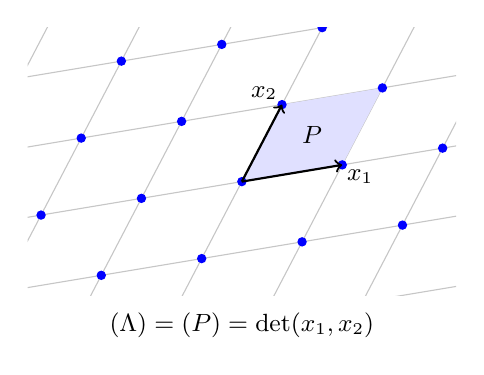
\begin{tikzpicture}[scale=0.85]
		\begin{scope}
			\clip (-3.2,-1.7) rectangle (3.2,2.3);
			\foreach \a in {-6,...,6}{
				\foreach \b in {-4,...,4}{
					\draw[gray!45] ({1.5*\a+0.6*\b},{0.25*\a+1.15*\b}) -- ({1.5*(\a+1)+0.6*\b},{0.25*(\a+1)+1.15*\b});
					\draw[gray!45] ({1.5*\a+0.6*\b},{0.25*\a+1.15*\b}) -- ({1.5*\a+0.6*(\b+1)},{0.25*\a+1.15*(\b+1)});
				}
			}
			\fill[blue!12] (0,0) -- (1.5,0.25) -- (2.1,1.4) -- (0.6,1.15) -- cycle;
			\foreach \a in {-6,...,6}{
				\foreach \b in {-4,...,4}{
					\fill[blue] ({1.5*\a+0.6*\b},{0.25*\a+1.15*\b}) circle (2pt);
				}
			}
		\end{scope}
		\draw[thick,->] (0,0) -- (1.5,0.25) node[below right=-2pt] {\small $x_1$};
		\draw[thick,->] (0,0) -- (0.6,1.15) node[above left=-2pt] {\small $x_2$};
		\node at (1.05,0.7) {\small $P$};
		\node at (0,-2.15) {\small $\covol(\Lambda) = \vol(P) = \abs{\det(x_1,x_2)}$};
	\end{tikzpicture}
\end{center}

\begin{example}
	$\Z^n \subseteq \R^n$ is a lattice of covolume $1$. On the other hand $\Z\sqrt2 + \Z\sqrt3 \subseteq \R$ is a subgroup that is \emph{not} discrete -- it is dense, by an argument with continued fractions -- and correspondingly it is not free of rank $1$.
\end{example}

\subsection{Minkowski's Theorem}

\begin{theorem}[Minkowski]\label{nf-thm:minkowski}
	Let $\Lambda \subseteq \R^n$ be a lattice and $S \subseteq \R^n$ measurable.
	\begin{enumerate}[label=(\roman*)]
		\item If $\vol(S) > \covol(\Lambda)$ then there exist $x \neq y$ in $S$ with $x - y \in \Lambda$.
		\item Suppose in addition that $S$ is convex and symmetric about $0$ (that is, $s \in S \Rightarrow -s \in S$). If either
		\begin{enumerate}[label=(\alph*)]
			\item $\vol(S) > 2^n\covol(\Lambda)$, or
			\item $\vol(S) \geq 2^n\covol(\Lambda)$ and $S$ is closed and bounded,
		\end{enumerate}
		then $S$ contains a nonzero point of $\Lambda$.
	\end{enumerate}
\end{theorem}

\begin{proof}
	(i) Let $P$ be a fundamental parallelotope. Since the translates $\gamma + P$ ($\gamma \in \Lambda$) partition $\R^n$,
	$$\vol(S) = \sum_{\gamma\in\Lambda}\vol\left(S \cap (P+\gamma)\right) = \sum_{\gamma\in\Lambda}\vol\left((S-\gamma)\cap P\right),$$
	by translation invariance of volume. If the sets $(S-\gamma)\cap P$ were pairwise disjoint, they would all sit inside $P$ and we would get $\vol(P) \geq \vol(S)$, contrary to hypothesis. So there are $\gamma \neq \mu$ in $\Lambda$ and a point in $(S-\gamma)\cap(S-\mu)$, i.e.\ there are $x, y \in S$ with $x - \gamma = y - \mu$. Then $x - y = \gamma-\mu \in\Lambda\setminus\{0\}$, so in particular $x \neq y$.

	(ii)(a) Apply (i) to $S' = \tfrac12S$, which has $\vol(S') = 2^{-n}\vol(S) > \covol(\Lambda)$. So there are $y \neq z \in S'$ with $y - z \in \Lambda\setminus\{0\}$. But $2y, 2z \in S$, so $-2z \in S$ by symmetry, and
	$$y - z = \tfrac12(2y) + \tfrac12(-2z) \in S$$
	by convexity. So $y - z$ is a nonzero lattice point in $S$.

	(ii)(b) For each integer $m \geq 1$ apply (a) to $S_m = (1+\tfrac1m)S$, which is convex, symmetric and of volume $(1+\tfrac1m)^n\vol(S) > 2^n\covol(\Lambda)$. This gives $\gamma_m \in (S_m \cap \Lambda)\setminus\{0\}$. Now $S_m \subseteq S_1 = 2S$ for all $m$ (by convexity and $0 \in S$), and $S_1\cap\Lambda$ is finite since $S_1$ is compact and $\Lambda$ discrete. So some value $\gamma$ occurs infinitely often among the $\gamma_m$, and then
	$$\gamma \in \bigcap_{m\ge1}S_m = \overline{S} = S$$
	as $S$ is closed. Hence $\gamma \in (S\cap\Lambda)\setminus\{0\}$.
\end{proof}

Here is part (ii)(a) in a picture. The shaded region is $S' = \tfrac12 S$; if its area exceeds the covolume then two of its points differ by a lattice vector, and doubling turns that into a lattice point inside $S$ itself.

\begin{center}
	\begin{tikzpicture}[scale=0.9]
		\begin{scope}
			\clip (-3.3,-2.3) rectangle (3.3,2.3);
			\foreach \a in {-4,...,4}{
				\foreach \b in {-3,...,3}{
					\fill[blue] (\a*1.4,\b*1.15) circle (1.7pt);
				}
			}
		\end{scope}
		\draw[thick, red] (0,0) ellipse (2.9 and 1.95);
		\draw[thick, red!45, dashed] (0,0) ellipse (1.45 and 0.975);
		\fill[red!10, opacity=0.5] (0,0) ellipse (1.45 and 0.975);
		\fill[red] (1.4,1.15) circle (2.4pt);
		\fill[red] (-1.4,-1.15) circle (2.4pt);
		\node[right=2pt, red] at (2.9,0.35) {\small $S$};
		\node[right=1pt, red!70] at (1.45,-0.42) {\small $\tfrac12 S$};
		\node[above right=-1pt] at (1.4,1.15) {\small $\gamma$};
		\node at (0,-2.65) {\small $\vol(S) > 2^n\covol(\Lambda) \implies$ some $0 \neq \gamma \in S\cap\Lambda$};
	\end{tikzpicture}
\end{center}

\begin{remark}
	The bounds are sharp. Take $\Lambda = \Z^n$, so $\covol(\Lambda) = 1$, and $S = (-1,1)^n$, which is open, convex, symmetric, of volume exactly $2^n$, and contains no nonzero lattice point. Closing it up to $[-1,1]^n$ makes case (b) apply, and indeed $\pm e_i \in S\cap\Lambda$.
\end{remark}

\subsection{The Minkowski Embedding}

We now put $K$ into a Euclidean space. Let $K$ have degree $n$ and signature $(r,s)$, with embeddings $\sigma_1,\dots,\sigma_r : K \to \R$ and $\sigma_{r+1},\dots,\sigma_{r+s} : K \to \C$ (one from each conjugate pair). Define
$$\sigma : K \longrightarrow \R^r\times\C^s \cong \R^{r+2s} = \R^n,$$
$$\sigma(x) = \left(\sigma_1(x),\dots,\sigma_r(x),\ \re\sigma_{r+1}(x),\im\sigma_{r+1}(x),\ \dots,\ \re\sigma_{r+s}(x),\im\sigma_{r+s}(x)\right).$$
This is an injective $\Q$-linear map, called the \vocab{Minkowski embedding}. Its whole purpose is the following.

\begin{lemma}\label{lem:latticecovol}
	Let $\fa \trianglelefteq \OO_K$ be a nonzero ideal. Then $\sigma(\fa)$ is a lattice in $\R^n$, with
	$$\covol(\sigma(\fa)) = 2^{-s}\abs{d_K}^{1/2}\,\Nm(\fa).$$
	In particular $\covol(\sigma(\OO_K)) = 2^{-s}\abs{d_K}^{1/2}$.
\end{lemma}

\begin{proof}
	Let $\gamma_1,\dots,\gamma_n$ be a $\Z$-basis of $\fa$. Then $\sigma(\fa) = \bigoplus_i\Z\sigma(\gamma_i)$, so it suffices to compute $\abs{\det(\sigma(\gamma_1),\dots,\sigma(\gamma_n))}$ and check it is nonzero.

	Consider first the matrix $S = (\sigma_i(\gamma_j))$ where now $\sigma_1,\dots,\sigma_n$ runs over \emph{all} $n$ embeddings. By Lemma \ref{lem:idealdisc},
	$$(\det S)^2 = \Delta(\gamma_1,\dots,\gamma_n) = \Nm(\fa)^2 d_K, \qquad \text{so } \abs{\det S} = \Nm(\fa)\abs{d_K}^{1/2} \neq 0.$$
	The matrix of $\sigma$ differs from $S$ by replacing each conjugate pair of rows $(z, \bar z)$ by $(\re z, \im z)$, and
	$$\begin{pmatrix}\re z\\ \im z\end{pmatrix} = \frac12\begin{pmatrix}1 & 1\\ -i & i\end{pmatrix}\begin{pmatrix}z \\ \bar z\end{pmatrix},$$
	a matrix of determinant $\tfrac12 \cdot \tfrac{1}{2}(i+i)= \tfrac{i}{2}$, of absolute value $\tfrac12$. Doing this for each of the $s$ pairs multiplies the absolute determinant by $2^{-s}$, giving
	$$\covol(\sigma(\fa)) = 2^{-s}\Nm(\fa)\abs{d_K}^{1/2} \neq 0,$$
	which in particular shows $\sigma(\gamma_1),\dots,\sigma(\gamma_n)$ are $\R$-independent, so $\sigma(\fa)$ is a lattice.
\end{proof}

\begin{example}
	For $K$ imaginary quadratic, $(r,s) = (0,1)$ and $\sigma$ is just the inclusion $K \subseteq \C = \R^2$ (after choosing a square root of $d$), which is what we drew for $\Z[i]$ and $\Z[\omega]$ in Section 1. The lemma says $\covol(\OO_K) = \tfrac12\abs{d_K}^{1/2}$: for $\Z[i]$, $d_K = -4$ gives covolume $1$, correct for the unit square lattice; for $\Z[\omega]$, $d_K=-3$ gives $\tfrac{\sqrt3}{2}$, correct for the triangular lattice with unit side.

	For $K = \Q(\sqrt d)$ real quadratic, $(r,s) = (2,0)$ and $\sigma(x) = (x, \bar x)$ using the two real embeddings; here $\covol(\OO_K) = \abs{d_K}^{1/2}$. For instance $\sigma(\Z[\sqrt2])$ is the lattice spanned by $(1,1)$ and $(\sqrt2,-\sqrt2)$, of covolume $2\sqrt2 = \sqrt 8 = \abs{d_K}^{1/2}$.
\end{example}

The reason this embedding is the right one is that the norm becomes a product of coordinates:
$$\Nm_{K/\Q}(x) = \prod_{i=1}^r\sigma_i(x)\prod_{j=1}^s\abs{\sigma_{r+j}(x)}^2,$$
so bounding $\abs{\Nm(x)}$ is bounding a product of coordinates -- exactly the sort of thing the AM--GM inequality handles.

\subsection{The Minkowski Bound}

\begin{proposition}[Minkowski Bound]\label{prop:minkbound}
	Let $K$ be a number field of degree $n$ and signature $(r,s)$, and let $\fa \trianglelefteq \OO_K$ be a nonzero ideal. Then there is $\alpha \in \fa$, $\alpha \neq 0$, with
	$$\abs{\Nm_{K/\Q}(\alpha)} \le C_K\,\Nm(\fa), \qquad \text{where } C_K = \left(\frac4\pi\right)^{\!s}\frac{n!}{n^n}\abs{d_K}^{1/2}$$
	is the \vocab{Minkowski constant} of $K$.
\end{proposition}

\begin{proof}
	For $t > 0$ let
	$$B(t) = \left\{(y_1,\dots,y_r,z_1,\dots,z_s) \in \R^r\times\C^s\ :\ \sum_{i=1}^r\abs{y_i} + 2\sum_{j=1}^s\abs{z_j} \le t\right\}.$$
	This set is closed, bounded, convex and symmetric about $0$, and (see below) has volume
	$$\vol(B(t)) = 2^r\left(\frac\pi2\right)^{\!s}\frac{t^n}{n!}.$$
	Choose $t$ so that $\vol(B(t)) = 2^n\covol(\sigma(\fa)) = 2^n2^{-s}\abs{d_K}^{1/2}\Nm(\fa)$; solving,
	$$t^n = \left(\frac4\pi\right)^{\!s}n!\,\abs{d_K}^{1/2}\Nm(\fa),$$
	using $n - r - s = s$. By Minkowski's theorem \ref{nf-thm:minkowski}(ii)(b) there is a nonzero $\alpha \in \fa$ with $\sigma(\alpha) \in B(t)$.

	Write $\sigma(\alpha) = (y_1,\dots,y_r,z_1,\dots,z_s)$. Then $\abs{\Nm(\alpha)} = \prod_i\abs{y_i}\prod_j\abs{z_j}^2$, a product of $n$ nonnegative reals whose sum is at most $t$. By AM--GM,
	$$\abs{\Nm(\alpha)}^{1/n} \le \frac1n\left(\sum_i\abs{y_i}+2\sum_j\abs{z_j}\right)\le\frac tn,$$
	so $\abs{\Nm(\alpha)} \le t^n/n^n = C_K\Nm(\fa)$.
\end{proof}

It remains to justify the volume formula, which we do by induction.

\begin{lemma}\label{lem:volB}
	Write $B_{r,s}(t)$ for the set above, sitting in $\R^r\times\C^s \cong \R^{n}$ with $n = r+2s$. Then
	$$\vol\left(B_{r,s}(t)\right) = 2^r\left(\frac{\pi}{2}\right)^{\!s}\frac{t^n}{n!}.$$
\end{lemma}

\begin{proof}
	We induct on $r+s$. If $r+s = 1$ there are two cases. For $(r,s) = (1,0)$, $B_{1,0}(t) = [-t,t]$ has length $2t$, matching $2^1t^1/1!$. For $(r,s) = (0,1)$, $B_{0,1}(t) = \{z \in \C : 2\abs z \le t\}$ is a disc of radius $t/2$ and area $\pi t^2/4$, matching $(\pi/2)t^2/2!$.

	For the inductive step in the real direction, slice along the new real coordinate $y$: the slice at height $y$ is $B_{r,s}(t-\abs y)$, so
	\begin{align*}
		\vol\left(B_{r+1,s}(t)\right) &= \int_{-t}^{t}\vol\left(B_{r,s}(t-\abs y)\right)\dd y = 2\int_0^t 2^r\left(\frac\pi2\right)^{\!s}\frac{(t-y)^{n}}{n!}\dd y\\
		&= 2^{r+1}\left(\frac\pi2\right)^{\!s}\frac{t^{n+1}}{(n+1)!},
	\end{align*}
	which is the formula in dimension $n+1$.

	In the complex direction, slice along the new complex coordinate $z$ and write $z = \tfrac12\rho e^{i\theta}$, so that the constraint reads $\rho \le t$ and the slice is $B_{r,s}(t-\rho)$. The area element is $\abs z \dd\abs z\dd\theta = \tfrac14\rho\dd\rho\dd\theta$, so
	$$\vol\left(B_{r,s+1}(t)\right) = \int_0^{2\pi}\!\!\int_0^t \frac{\rho}{4}\,\vol\left(B_{r,s}(t-\rho)\right)\dd\rho\dd\theta = \frac{2\pi}{4}\cdot2^r\left(\frac\pi2\right)^{\!s}\int_0^t\frac{\rho\,(t-\rho)^n}{n!}\dd\rho.$$
	Now $\int_0^t\rho(t-\rho)^n\dd\rho = t^{n+2}/((n+1)(n+2))$ by the substitution $\rho \mapsto t-\rho$ and the beta integral, so the right-hand side is $2^r(\pi/2)^{s+1}t^{n+2}/(n+2)!$, as required.
\end{proof}

\subsection{Finiteness of the Class Group}

\begin{theorem}[Finiteness of the Class Group]\label{thm:finiteclass}
	Let $K$ be a number field. Then every ideal class of $K$ contains an integral ideal $\fb$ with $\Nm(\fb) \le C_K$. Consequently $\Cl_K$ is finite, and it is generated by the classes of the prime ideals $\fp$ with $\Nm(\fp) \le C_K$.
\end{theorem}

\begin{proof}
	Let $c \in \Cl_K$ and pick an integral ideal $\fa$ with $[\fa] = c^{-1}$ (possible: any fractional ideal in $c^{-1}$ can be scaled into $\OO_K$). By Proposition \ref{prop:minkbound} there is $0 \neq \alpha\in\fa$ with $\abs{\Nm(\alpha)} \le C_K\Nm(\fa)$. Since $\alpha \in \fa$ we have $(\alpha) \subseteq \fa$, so $(\alpha) = \fa\fb$ for some integral ideal $\fb$ (Corollary \ref{cor:containdivide}). Taking norms and using Lemma \ref{lem:normprincipal},
	$$\Nm(\fa)\Nm(\fb) = \Nm((\alpha)) = \abs{\Nm(\alpha)} \le C_K\Nm(\fa),$$
	so $\Nm(\fb) \le C_K$. And $[\fb] = [\fa]^{-1} = c$ since $\fa\fb$ is principal.

	For finiteness: by Corollary \ref{cor:normbounds}(i) there are only finitely many ideals of norm at most $C_K$, so there are only finitely many classes. For the generation statement, if $\Nm(\fb)\le C_K$ and $\fb = \prod\fp_i^{a_i}$, then each $\Nm(\fp_i) \le \Nm(\fb) \le C_K$ by multiplicativity, so $[\fb]$ is a product of classes of small-norm primes.
\end{proof}

This is a genuinely remarkable theorem, and it gives a completely effective algorithm: to compute $\Cl_K$, list the primes $p \le C_K$, factor each $(p)$ using Dedekind's criterion, and then find the relations among the resulting classes. We will do this in Section \ref{sec:computing}.

\begin{example}
	For $K$ imaginary quadratic, $n=2$, $s=1$ and $C_K = \frac{2}{\pi}\abs{d_K}^{1/2}$. For $K$ real quadratic, $s = 0$ and $C_K = \tfrac12\abs{d_K}^{1/2}$. For $K = \Q(\sqrt{-7})$, $d_K = -7$ and $C_K = 2\sqrt7/\pi \approx 1.68 < 2$, so there are no primes of norm $\le C_K$ at all and $\Cl_K$ is trivial: $\Z[\tfrac12(1+\sqrt{-7})]$ is a PID. The same works for $d = -1,-2,-3$.
\end{example}

The Minkowski bound also gives a lower bound for the discriminant, since applying it to the trivial class produces an ideal of norm at least $1$.

\begin{theorem}[Hermite--Minkowski]\label{thm:hermite}
	Let $K$ be a number field of degree $n \geq 2$. Then
	$$\abs{d_K} \ge \frac{\pi}{3}\left(\frac{3\pi}{4}\right)^{n-1} > 1.$$
	In particular $\abs{d_K} > 1$, so by Theorem \ref{thm:ramdisc} at least one prime ramifies in $K$.
\end{theorem}

\begin{proof}
	Applying Theorem \ref{thm:finiteclass} to the trivial class gives an ideal $\fb$ with $1 \le \Nm(\fb)\le C_K$, so $C_K \ge 1$, i.e.
	$$\abs{d_K}^{1/2} \ge \left(\frac\pi4\right)^{\!s}\frac{n^n}{n!} \ge \left(\frac\pi4\right)^{\!n/2}\frac{n^n}{n!} =: a_n^{1/2},$$
	using $\pi/4 < 1$ and $s \le n/2$. Now $a_n = \left(\frac\pi4\right)^{n}\left(\frac{n^n}{n!}\right)^2$ satisfies $a_2 = \frac{\pi^2}{4}$ and
	$$\frac{a_{n+1}}{a_n} = \frac\pi4\left(1+\frac1n\right)^{2n} \ge \frac{\pi}{4}\cdot 4 = \pi > \frac{3\pi}{4},$$
	since $(1+1/n)^n \ge 2$ for $n \ge 1$. Hence
	$$a_n \ge \frac{\pi^2}{4}\left(\frac{3\pi}{4}\right)^{n-2} = \frac\pi3\left(\frac{3\pi}{4}\right)^{n-1},$$
	and $\frac\pi3\cdot\frac{3\pi}{4} = \frac{\pi^2}{4} > 2$, so the bound exceeds $1$ for all $n \ge 2$.
\end{proof}

\begin{remark}
	Minkowski's theorem also implies (with more work) \vocab{Hermite's theorem}: for each $D$ there are only finitely many number fields with $\abs{d_K}\le D$. So the discriminant is a genuinely rigid invariant. The smallest discriminants in absolute value in low degree are $-3$ (for $\Q(\sqrt{-3})$), $-23$ (for the cubic field $\Q(\alpha)$ with $\alpha^3=\alpha+1$, whose discriminant we computed in Section 2) and $117$ in degree $4$; compare these with the bound above, which gives $\abs{d_K} \geq 2.4, 5.8, 13.7$ for $n = 2,3,4$.
\end{remark}

\section{Computing Class Groups}\label{sec:computing}

Theorem \ref{thm:finiteclass} turns the computation of $\Cl_K$ into a finite, mechanical procedure. Let us set out the recipe and then run it several times.

\begin{enumerate}[label=(\arabic*)]
	\item Compute $d_K$ and the Minkowski constant $C_K = \left(\tfrac4\pi\right)^s\tfrac{n!}{n^n}\abs{d_K}^{1/2}$.
	\item For each rational prime $p \le C_K$, factor $p\OO_K$ using Dedekind's criterion. The primes $\fp$ with $\Nm(\fp) \le C_K$ obtained this way generate $\Cl_K$.
	\item Decide which of these $\fp$ are principal, usually by asking whether there is $\alpha \in \OO_K$ with $\abs{\Nm(\alpha)} = \Nm(\fp)$ -- a norm-form equation.
	\item Find relations. The most efficient source of relations is to factor $(\alpha)$ for elements $\alpha$ of small norm: each such factorisation is a relation in $\Cl_K$.
\end{enumerate}

Throughout, we use freely that in a quadratic field $[\bar\fa] = [\fa]^{-1}$ (Example \ref{ex:conjinverse}), and that $\Nm(a+b\sqrt d) = a^2-db^2$.

\begin{example}[$K = \Q(\sqrt{-5})$]\label{ex:cl5}
	Here $d_K = -20$ and $C_K = \tfrac2\pi\sqrt{20} \approx 2.847$. So $\Cl_K$ is generated by primes of norm $\le 2$, i.e.\ primes above $2$. By Example \ref{ex:quadfactor}, $(2) = \fp^2$ with $\fp = (2,1+\sqrt{-5})$ of norm $2$.

	Is $\fp$ principal? If $\fp = (\beta)$ then $\Nm(\beta) = \pm2$, i.e.\ $a^2+5b^2 = 2$, which is insoluble. So $[\fp]\neq1$, while $[\fp]^2 = [(2)] = 1$. Hence
	$$\Cl_{\Q(\sqrt{-5})} \cong \Z/2\Z, \qquad h_K = 2.$$
	In particular $\Z[\sqrt{-5}]$ is not a UFD, which we knew, and the failure is as mild as it could possibly be.
\end{example}

\begin{example}[$K = \Q(\sqrt{-23})$]\label{ex:cl23}
	Here $-23 \equiv 1\pmod 4$, so $d_K = -23$, $\OO_K = \Z[\alpha]$ with $\alpha = \tfrac12(1+\sqrt{-23})$ of minimal polynomial $x^2-x+6$, and $C_K = \tfrac2\pi\sqrt{23}\approx 3.05$. So we need the primes above $2$ and $3$.

	Modulo $2$: $x^2-x+6 \equiv x^2+x = x(x+1)$, so $(2) = \fp\bar\fp$ with $\fp = (2,\alpha)$, $\bar\fp = (2,\alpha-1)$, each of norm $2$. Modulo $3$: $x^2-x+6\equiv x^2-x = x(x-1)$, so $(3) = \fq\bar\fq$ with $\fq = (3,\alpha)$, $\bar\fq = (3,\alpha-1)$, each of norm $3$.

	Norms of elements: $\Nm\left(\tfrac12(u+v\sqrt{-23})\right) = \tfrac14(u^2+23v^2)$ with $u \equiv v \pmod 2$. So $\Nm(\gamma) = m$ requires $u^2+23v^2 = 4m$. For $m = 2$: $u^2+23v^2 = 8$ is insoluble, so $\fp$ is not principal. For $m = 3$: $u^2+23v^2 = 12$ is insoluble, so $\fq$ is not principal. For $m=4$: $u^2+23v^2=16$ forces $v = 0, u = \pm4$, giving $\gamma = \pm 2$ and $(\gamma) = (2) = \fp\bar\fp$; so $\fp^2$ is not principal either (if it were, $\fp^2 = (\gamma)$ with $\Nm(\gamma) = 4$, forcing $\fp^2 = (2) = \fp\bar\fp$ and so $\fp = \bar\fp$, false).

	Now for a relation. Take $m = 6$: $u^2+23v^2 = 24$ has the solution $u = v = 1$, giving
	$$\gamma = \tfrac12(1+\sqrt{-23}) = \alpha, \qquad \Nm(\alpha) = 6.$$
	Since $\alpha \in \fp$ and $\alpha \in \fq$, we get $(\alpha) = \fp\fq$. Hence $[\fq] = [\fp]^{-1}$, so $\Cl_K = \langle[\fp]\rangle$ is cyclic.

	Finally take $m=8$: the equation $u^2+23v^2=32$ has the solution $u = 3, v = 1$, giving $\beta = \tfrac12(3+\sqrt{-23})$ with $\Nm(\beta) = 8$. Now $(\beta)$ has norm $8 = 2^3$, so it is a product of three primes above $2$, that is $(\beta) = \fp^a\bar\fp^{\,3-a}$. If both $\fp$ and $\bar\fp$ occurred then $(2) = \fp\bar\fp$ would divide $(\beta)$, forcing $\beta/2 = \tfrac14(3+\sqrt{-23}) \in \OO_K$; but that element has norm $2$, which we have seen is impossible. So $(\beta) = \fp^3$ or $\bar\fp^{\,3}$, and either way $[\fp]^3 = 1$.

	Since $[\fp] \ne 1$ and $[\fp]^2\neq1$, the class $[\fp]$ has order $3$, and
	$$\Cl_{\Q(\sqrt{-23})}\cong\Z/3\Z, \qquad h_K = 3.$$
\end{example}

\begin{example}[$K = \Q(\sqrt{-17})$]\label{ex:cl17}
	Here $-17\equiv3\pmod4$, so $d_K = -68$, $\OO_K = \Z[\sqrt{-17}]$ and $C_K = \tfrac2\pi\sqrt{68}\approx5.25$. We need the primes above $2, 3, 5$.
	\begin{itemize}
		\item $p=2$: $x^2+17\equiv x^2+1 = (x+1)^2 \pmod 2$, so $(2) = \fp^2$ with $\fp = (2,1+\sqrt{-17})$, $\Nm(\fp) = 2$.
		\item $p=3$: $x^2+17\equiv x^2-1 = (x-1)(x+1)\pmod3$, so $(3) = \fq\bar\fq$ with $\fq = (3,1+\sqrt{-17})$, $\Nm(\fq)=3$.
		\item $p=5$: $x^2+17\equiv x^2+2 \pmod 5$, and $-2\equiv3$ is not a square mod $5$, so $5$ is inert and contributes the trivial class.
	\end{itemize}
	Now $\Nm(a+b\sqrt{-17}) = a^2+17b^2$, which never equals $2$ or $3$, so neither $\fp$ nor $\fq$ is principal. For a relation, note
	$$\Nm(1+\sqrt{-17}) = 18 = 2\cdot3^2.$$
	Since $1+\sqrt{-17}$ lies in both $\fp$ and $\fq$, and the only primes of norm $2$ and $3$ dividing $(1+\sqrt{-17})$ are $\fp$ and $\fq,\bar\fq$, we must have $(1+\sqrt{-17}) = \fp\fq^2$ (it cannot involve both $\fq$ and $\bar\fq$, since $\fq\bar\fq = (3)$ and $3 \nmid 1+\sqrt{-17}$). Hence in $\Cl_K$,
	$$[\fp][\fq]^2 = 1, \qquad [\fp]^2 = 1,$$
	so $[\fq]^4 = [\fp]^{-2} = 1$ and $[\fq]^2 = [\fp]^{-1} = [\fp] \ne 1$. Therefore $[\fq]$ has order $4$, and since $\Cl_K = \langle[\fp],[\fq]\rangle = \langle[\fq]\rangle$,
	$$\Cl_{\Q(\sqrt{-17})} \cong \Z/4\Z, \qquad h_K = 4.$$
\end{example}

\begin{example}[$K = \Q(\sqrt{-14})$]
	Here $d_K = -56$ and $C_K = \tfrac2\pi\sqrt{56}\approx 4.76$, so we need primes above $2$ and $3$. Modulo $2$, $x^2+14\equiv x^2$, so $(2) = \fp^2$ with $\fp = (2,\sqrt{-14})$. Modulo $3$, $x^2+14\equiv x^2+2\equiv x^2-1$, so $(3) = \fq\bar\fq$ with $\fq = (3,1+\sqrt{-14})$.

	Neither is principal, since $a^2+14b^2 \in \{2,3\}$ is insoluble. But $\Nm(2+\sqrt{-14}) = 18 = 2\cdot3^2$ and $2+\sqrt{-14} \in\fp$, so exactly as before $(2+\sqrt{-14}) = \fp\fq^2$ (up to replacing $\fq$ by $\bar\fq$). So $[\fq]^4=1$ and $[\fq]^2 = [\fp]\ne1$, giving
	$$\Cl_{\Q(\sqrt{-14})}\cong\Z/4\Z, \qquad h_K = 4.$$
\end{example}

Real quadratic fields work the same way, but the Minkowski constant is smaller by a factor of $8/\pi$, which often makes life easier.

\begin{example}[$K = \Q(\sqrt{10})$]\label{ex:cl10}
	Here $10 \equiv 2\pmod4$, so $d_K = 40$, $\OO_K = \Z[\sqrt{10}]$, and $C_K = \tfrac12\sqrt{40}\approx3.16$. We need the primes above $2$ and $3$.
	\begin{itemize}
		\item $p=2$: $x^2-10\equiv x^2\pmod2$, so $(2) = \fp^2$ with $\fp = (2,\sqrt{10})$, $\Nm(\fp)=2$.
		\item $p=3$: $x^2-10\equiv x^2-1 = (x-1)(x+1)\pmod 3$, so $(3) = \fq\bar\fq$ with $\fq = (3,\sqrt{10}-1)$, $\Nm(\fq)=3$.
	\end{itemize}
	Now $\Nm(a+b\sqrt{10}) = a^2-10b^2$. If this is $\pm2$ then $a^2\equiv\pm2\pmod 5$; but the squares mod $5$ are $0,1,4$, and $\pm2 \equiv 2, 3$. So $\fp$ is not principal. Likewise $a^2-10b^2 = \pm3$ forces $a^2 \equiv \pm3 \equiv 3, 2 \pmod 5$, impossible; so $\fq$ is not principal.

	For a relation, $\Nm(2+\sqrt{10}) = 4-10 = -6$, so $(2+\sqrt{10}) = \fp\fq$ or $\fp\bar\fq$. Either way $[\fq] = [\fp]^{-1} = [\fp]$ (as $[\fp]^2 = 1$), so $\Cl_K = \langle[\fp]\rangle$ has order $2$:
	$$\Cl_{\Q(\sqrt{10})}\cong\Z/2\Z, \qquad h_K = 2.$$
	Concretely, the failure of unique factorisation is visible in
	$$6 = 2\cdot 3 = \left(\sqrt{10}+2\right)\left(\sqrt{10}-2\right),$$
	where all four factors are irreducible (their norms are $4, 9, 6, 6$, and $a^2-10b^2 = \pm2,\pm3$ are insoluble) and no two are associates. The ideal-theoretic resolution is
	$$(6) = \fp^2\fq\bar\fq, \qquad (2) = \fp^2,\ (3) = \fq\bar\fq,\ \left(\sqrt{10}+2\right) = \fp\fq,\ \left(\sqrt{10}-2\right) = \fp\bar\fq,$$
	exactly as in the $\Q(\sqrt{-5})$ story.
\end{example}

\begin{example}[$K = \Q(\sqrt{-6})$]
	Here $d_K = -24$ and $C_K = \tfrac2\pi\sqrt{24}\approx3.12$, so we need primes above $2$ and $3$. Both ramify: $x^2+6 \equiv x^2 \pmod 2$ and $\pmod 3$, so
	$$(2) = \fp_2^{\,2}, \quad \fp_2 = \left(2,\sqrt{-6}\right); \qquad (3) = \fp_3^{\,2}, \quad \fp_3 = \left(3,\sqrt{-6}\right).$$
	Neither is principal, as $a^2+6b^2 \in \{2,3\}$ is insoluble. But $\Nm(\sqrt{-6}) = 6$, and $\sqrt{-6}$ lies in both, so $(\sqrt{-6}) = \fp_2\fp_3$ and hence $[\fp_3] = [\fp_2]^{-1} = [\fp_2]$. So $\Cl_K = \langle[\fp_2]\rangle$ has order $2$ and $h_K = 2$.
\end{example}

\begin{example}[$K = \Q(\sqrt{15})$]
	Here $15 \equiv 3\pmod4$, so $d_K = 60$, $\OO_K = \Z[\sqrt{15}]$ and $C_K = \tfrac12\sqrt{60}\approx3.87$: again the primes above $2$ and $3$. Modulo $2$, $x^2-15 \equiv x^2+1 = (x+1)^2$, so $(2) = \fp_2^{\,2}$ with $\fp_2 = (2,1+\sqrt{15})$; modulo $3$, $x^2-15\equiv x^2$, so $(3) = \fp_3^{\,2}$ with $\fp_3 = (3,\sqrt{15})$.

	For principality we need $a^2-15b^2 = \pm2$ or $\pm3$. Reducing mod $5$ gives $a^2 \equiv \pm2$ or $\pm3$, i.e.\ $a^2 \in \{2,3\}$ mod $5$; but the squares mod $5$ are $0,1,4$. So neither prime is principal. Finally $\Nm(3+\sqrt{15}) = 9-15 = -6$, and $3+\sqrt{15}$ lies in both $\fp_2$ and $\fp_3$, so $(3+\sqrt{15}) = \fp_2\fp_3$ and $[\fp_3]=[\fp_2]$. Hence
	$$\Cl_{\Q(\sqrt{15})}\cong\Z/2\Z, \qquad h_K = 2.$$
\end{example}

\begin{example}[A Non-Cyclic Class Group: $K = \Q(\sqrt{-30})$]
	All our examples so far have had cyclic class group, which is a little misleading. Here $d_K = -120$ and $C_K = \tfrac2\pi\sqrt{120}\approx 6.97$, so we need the primes above $2,3,5$. All three divide $d_K$, so all three ramify:
	$$(2) = \fp_2^{\,2},\qquad (3) = \fp_3^{\,2},\qquad (5) = \fp_5^{\,2},$$
	$$\fp_2 = \left(2,\sqrt{-30}\right),\qquad \fp_3 = \left(3,\sqrt{-30}\right),\qquad \fp_5 = \left(5,\sqrt{-30}\right).$$
	None is principal, since $a^2+30b^2 \in \{2,3,5\}$ is insoluble; so each class $[\fp_i]$ has order exactly $2$. Also $\Nm(\sqrt{-30}) = 30$ and $\sqrt{-30}$ lies in all three primes, so
	$$\left(\sqrt{-30}\right) = \fp_2\fp_3\fp_5, \qquad\text{giving}\qquad [\fp_2][\fp_3][\fp_5] = 1.$$
	So $\Cl_K = \langle[\fp_2],[\fp_3]\rangle$, a quotient of $\Z/2\Z\times\Z/2\Z$. Finally $[\fp_2][\fp_3] \neq 1$, since $\fp_2\fp_3$ has norm $6$ and $a^2+30b^2 = 6$ is insoluble. Hence
	$$\Cl_{\Q(\sqrt{-30})} \cong \Z/2\Z\times\Z/2\Z, \qquad h_K = 4.$$
	Notice how the ramified primes did all the work: this is typical, and is the beginning of \vocab{genus theory}, which computes the $2$-torsion of $\Cl_K$ for a quadratic field purely in terms of the number of prime divisors of $d_K$.
\end{example}

\begin{example}[Fields of Class Number One]
	If $C_K < 2$ there are no primes to consider at all and $h_K = 1$ automatically. For imaginary quadratic $K$ this reads $\tfrac2\pi\abs{d_K}^{1/2} < 2$, i.e.\ $\abs{d_K} < \pi^2 \approx 9.87$, which happens for $d = -1,-2,-3,-7$. A little more work handles $d = -11,-19,-43,-67,-163$. In fact these nine are all:
	\begin{theorem}[Baker--Heegner--Stark]
		$\OO_{\Q(\sqrt{-d})}$ is a UFD (equivalently a PID) for $d > 0$ squarefree precisely when
		$$d \in \{1,2,3,7,11,19,43,67,163\}.$$
	\end{theorem}
	This is a deep theorem, conjectured by Gauss and settled only in the 1960s. By contrast, it is conjectured -- and completely open -- that infinitely many \emph{real} quadratic fields have class number one; numerically they seem to be rather common.
\end{example}

\begin{example}[A Cubic Field]
	Let $K = \Q(\sqrt[3]2)$, with $n = 3$, $(r,s) = (1,1)$ and $d_K = -108$. Then
	$$C_K = \frac4\pi\cdot\frac{3!}{3^3}\cdot\sqrt{108} \approx 2.94,$$
	so $\Cl_K$ is generated by primes of norm $2$. From Example \ref{ex:cbrt2}, the only one is $\fp = (2,\sqrt[3]2) = (\sqrt[3]2)$, which is principal. Hence $h_K = 1$ and $\Z[\sqrt[3]2]$ is a PID.
\end{example}

\begin{example}[A Cyclotomic Field]
	Let $K = \Q(\zeta_5)$, with $n=4$, $(r,s) = (0,2)$ and $d_K = 125$. Then
	$$C_K = \left(\frac4\pi\right)^{\!2}\frac{4!}{4^4}\sqrt{125}\approx 1.70 < 2,$$
	so there are no prime ideals of norm at most $C_K$, and $h_K = 1$: the ring $\Z[\zeta_5]$ is a PID.

	For $\Q(\zeta_7)$ the bound is larger, $C_K = \left(\tfrac4\pi\right)^3\tfrac{6!}{6^6}\sqrt{7^5}\approx4.13$, so we must look at the primes of norm at most $4$. But the primes above $2$ have residue degree $3$ and hence norm $8$, the primes above $3$ have residue degree $6$ and hence norm $729$, and the unique prime above $7$ has norm $7$; so again there is nothing to consider and $h_K = 1$.

	This cannot go on forever -- for $\Q(\zeta_{11})$ the bound is already about $59$ -- but in fact $h_{\Q(\zeta_p)} = 1$ for all $p \le 19$. The first failure is $p = 23$, where $h = 3$; and the first \vocab{irregular} prime, meaning one with $p \mid h_{\Q(\zeta_p)}$, is $p = 37$. This is exactly where Kummer's proof of Fermat's Last Theorem breaks down (see Section \ref{sec:applications}).
\end{example}

\begin{remark}
	There is a classical dictionary, going back to Gauss, between ideal classes in $\Q(\sqrt D)$ and binary quadratic forms. To a form $q(x,y) = ax^2+bxy+cy^2$ with $a,b,c\in\Z$ and discriminant $D = b^2-4ac$, associate the ideal
	$$\fa_q = \left(a, \frac{-b+\sqrt D}{2}\right) \trianglelefteq \OO_{\Q(\sqrt D)}.$$
	For $D < 0$ and $a > 0$, one can show that $[\fa_q] = [\fa_{q'}]$ if and only if $q$ and $q'$ are equivalent under the action of $SL_2(\Z)$ on forms. So $h_K$ is the number of $SL_2(\Z)$-orbits of positive definite binary quadratic forms of discriminant $D$ -- Gauss's \emph{class number}, computed by his reduction theory long before ideals were invented. For example the two classes for $D = -20$ correspond to the reduced forms $x^2+5y^2$ and $2x^2+2xy+3y^2$.
\end{remark}

\section{Dirichlet's Unit Theorem}\label{sec:units}

We turn to the other end of the exact sequence
\begin{center}
	\begin{tikzcd}[column sep=1.4em]
		1 \arrow[r] & \OO_K^\times \arrow[r] & K^\times \arrow[r] & I_K \arrow[r] & \Cl_K \arrow[r] & 1,
	\end{tikzcd}
\end{center}
namely the unit group $\OO_K^\times$. We saw in Example \ref{ex:unitsimag} that imaginary quadratic fields have finite unit group, whereas $\Z[\sqrt2]^\times$ contains the infinite cyclic group generated by $1+\sqrt2$. Dirichlet's theorem explains this completely: the answer depends only on the signature.

\begin{definition}[Roots of Unity]
	Let $\mu_K = \{\alpha \in K : \alpha^m = 1 \text{ for some } m \geq 1\}$ be the group of roots of unity in $K$.
\end{definition}

\begin{theorem}[Dirichlet's Unit Theorem]\label{nf-thm:dirichlet}
	Let $K$ be a number field of signature $(r,s)$. Then $\mu_K$ is finite and cyclic, and
	$$\OO_K^\times \cong \mu_K \times \Z^{r+s-1}.$$
\end{theorem}

So for $K$ imaginary quadratic, $(r,s) = (0,1)$ and the rank is $0$: the unit group is finite, as we found. For $K$ real quadratic, $(r,s) = (2,0)$ and the rank is $1$, so $\OO_K^\times = \{\pm\varepsilon^n : n \in \Z\}$ for a single $\varepsilon$ -- this is the statement that Pell's equation has infinitely many solutions, all generated by one. For $K = \Q(\sqrt[3]2)$, $(r,s) = (1,1)$ and the rank is again $1$.

\subsection{The Logarithmic Embedding}

The Minkowski embedding turns multiplication into a product of coordinates, and the norm condition $\Nm(u) = \pm1$ into a multiplicative constraint. Taking logarithms turns this into a linear constraint, which is what we can attack with lattices.

\begin{definition}[Logarithmic Embedding]
	Let $K$ have signature $(r,s)$ with embeddings as above. Define
	$$\ell : K^\times \to \R^{r+s},$$
	$$\ell(x) = \left(\log\abs{\sigma_1(x)},\ \dots,\ \log\abs{\sigma_r(x)},\ 2\log\abs{\sigma_{r+1}(x)},\ \dots,\ 2\log\abs{\sigma_{r+s}(x)}\right).$$
\end{definition}

The factors of $2$ on the complex coordinates are there so that $\ell$ interacts correctly with the norm; and $\ell$ does not depend on which member of each conjugate pair we chose, since conjugates have the same absolute value. Since $\log\abs{ab} = \log\abs a+\log\abs b$, the map $\ell$ is a group homomorphism from $(K^\times,\times)$ to $(\R^{r+s},+)$.

\begin{lemma}\label{lem:logimage}
	Let $L = \ell(\OO_K^\times) \subseteq \R^{r+s}$. Then
	\begin{enumerate}[label=(\roman*)]
		\item $L$ is a discrete subgroup of $\R^{r+s}$;
		\item $\ker\left(\ell|_{\OO_K^\times}\right) = \mu_K$, which is a finite cyclic group;
		\item $L$ is contained in the hyperplane $H = \{(y_1,\dots,y_{r+s}) : \sum_iy_i = 0\}$.
	\end{enumerate}
\end{lemma}

\begin{proof}
	(i) and (ii). The map $\ell$ factors as
	$$\OO_K^\times \xhookrightarrow{\ \sigma\ } (\R^\times)^r\times(\C^\times)^s \xrightarrow{\ j\ } \R^{r+s},$$
	where $j(y_1,\dots,y_r,z_1,\dots,z_s) = (\log\abs{y_1},\dots,2\log\abs{z_s})$. For $A>0$,
	$$j^{-1}\left([-A,A]^{r+s}\right) = \left\{(y_i,z_j) : e^{-A}\le\abs{y_i}\le e^A,\ e^{-A/2}\le\abs{z_j}\le e^{A/2}\right\}$$
	is a closed and bounded, hence compact, subset of $\R^n$. Since $\sigma(\OO_K)$ is a lattice (Lemma \ref{lem:latticecovol}), hence discrete, the intersection of this compact set with $\sigma(\OO_K^\times) \subseteq \sigma(\OO_K)$ is finite. So $L \cap [-A,A]^{r+s}$ is finite for every $A$, which gives discreteness, and taking $A \to 0$ shows the kernel of $\ell$ on $\OO_K^\times$ is finite.

	A finite subgroup of $K^\times$ consists of elements of finite order, so $\ker\ell \subseteq \mu_K$; conversely every root of unity has all conjugates of absolute value $1$, so lies in $\ker\ell$. Hence $\ker\ell = \mu_K$ is finite. Finally, embedding $K \hookrightarrow \C$ realises $\mu_K$ as a finite subgroup of $\C^\times$, hence as a group of $m$th roots of unity for some $m$; subgroups of cyclic groups are cyclic.

	(iii) If $u \in \OO_K^\times$ then $\Nm(u) = \pm1$ by Lemma \ref{lem:unitnorm}, so
	$$0 = \log\abs{\Nm(u)} = \sum_{i=1}^r\log\abs{\sigma_i(u)} + \sum_{j=1}^s2\log\abs{\sigma_{r+j}(u)},$$
	which is exactly the statement that $\ell(u) \in H$. \qedhere
\end{proof}

Since $H \cong \R^{r+s-1}$, part (i) and Proposition \ref{prop:discrete} give $L \cong \Z^a$ for some $a \le r+s-1$. The content of Dirichlet's theorem is that $a$ is as large as possible.

\begin{theorem}[Dirichlet, Lattice Form]\label{thm:dirichletlattice}
	$L = \ell(\OO_K^\times)$ is a full lattice in $H \cong \R^{r+s-1}$; that is, $L \cong \Z^{r+s-1}$.
\end{theorem}

Granting this, Theorem \ref{nf-thm:dirichlet} follows at once: we have a short exact sequence
$$1 \to \mu_K \to \OO_K^\times \xrightarrow{\ \ell\ } L \to 0$$
with $L \cong \Z^{r+s-1}$ free, so the sequence splits and $\OO_K^\times \cong \mu_K\times\Z^{r+s-1}$.

Here is the picture for a field with $r+s = 3$ (for instance a totally real cubic field, where $(r,s)=(3,0)$): the image $L$ is a rank-$2$ lattice sitting inside the plane $y_1+y_2+y_3=0$.

\begin{center}
	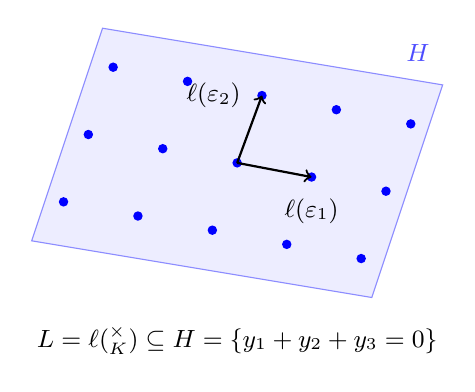
\begin{tikzpicture}[scale=0.9]
		% plane drawn as a parallelogram
		\fill[blue!7] (-2.9,-1.1) -- (1.9,-1.9) -- (2.9,1.1) -- (-1.9,1.9) -- cycle;
		\draw[blue!45] (-2.9,-1.1) -- (1.9,-1.9) -- (2.9,1.1) -- (-1.9,1.9) -- cycle;
		\foreach \a in {-2,...,2}{
			\foreach \b in {-1,...,1}{
				\fill[blue] ({1.05*\a+0.35*\b},{-0.2*\a+0.95*\b}) circle (1.9pt);
			}
		}
		\draw[thick,->] (0,0) -- (1.05,-0.2) node[below=4pt] {\small $\ell(\varepsilon_1)$};
		\draw[thick,->] (0,0) -- (0.35,0.95) node[left=4pt] {\small $\ell(\varepsilon_2)$};
		\node[blue!70] at (2.55,1.55) {\small $H$};
		\node at (0,-2.5) {\small $L = \ell(\OO_K^\times) \subseteq H = \{y_1+y_2+y_3=0\}$};
	\end{tikzpicture}
\end{center}

\subsection{Proof of Dirichlet's Theorem}

The strategy is to manufacture, for each coordinate $k$, a unit whose logarithmic image is negative in every coordinate except the $k$th. A linear algebra lemma then shows that such vectors are as independent as they can be. The manufacturing is done by Minkowski's theorem.

\begin{lemma}\label{lem:shrink}
	Fix $1 \le k \le r+s$ and let $0 \neq \alpha \in \OO_K$ with $\ell(\alpha) = (a_1,\dots,a_{r+s})$. Then there is $0 \neq \beta \in \OO_K$ with
	$$\abs{\Nm(\beta)} \le \left(\frac2\pi\right)^{\!s}\abs{d_K}^{1/2} \qquad\text{and}\qquad b_i < a_i \text{ for all } i \neq k,$$
	where $\ell(\beta) = (b_1,\dots,b_{r+s})$.
\end{lemma}

\begin{proof}
	For positive reals $c_1,\dots,c_{r+s}$ let
	$$S = \left\{(y_1,\dots,y_r,z_1,\dots,z_s) \in \R^r\times\C^s : \abs{y_i}\le c_i \ (i\le r),\ \abs{z_j}^2\le c_{r+j}\ (j \le s)\right\},$$
	a closed, bounded, convex, symmetric set of volume $\vol(S) = 2^r\pi^sc_1\cdots c_{r+s}$. Choose $c_i$ with $0 < c_i < e^{a_i}$ for $i \neq k$, and then define $c_k$ so that
	$$c_1c_2\cdots c_{r+s} = \left(\frac2\pi\right)^{\!s}\abs{d_K}^{1/2},$$
	which makes $\vol(S) = 2^r\pi^s(2/\pi)^s\abs{d_K}^{1/2} = 2^{r+s}\abs{d_K}^{1/2} = 2^n\covol(\sigma(\OO_K))$, using $r+2s = n$ and Lemma \ref{lem:latticecovol}. By Minkowski's theorem there is $0 \neq \beta \in \OO_K$ with $\sigma(\beta)\in S$. Then
	$$\abs{\Nm(\beta)} = \prod_{i\le r}\abs{y_i}\prod_{j\le s}\abs{z_j}^2 \le c_1\cdots c_{r+s} = \left(\frac2\pi\right)^{\!s}\abs{d_K}^{1/2},$$
	and for $i \neq k$ the $i$th coordinate of $\ell(\beta)$ is at most $\log c_i < a_i$.
\end{proof}

\begin{lemma}\label{lem:rank}
	Let $A = (a_{ij}) \in \mathrm{Mat}_{m}(\R)$ satisfy $a_{ii} > 0$, $a_{ij} < 0$ for $i \neq j$, and $\sum_j a_{ij} \geq 0$ for all $i$. Then $\rank A \geq m-1$.
\end{lemma}

\begin{proof}
	We show the first $m-1$ columns $v_1,\dots,v_{m-1}$ are linearly independent. Suppose $\sum_{i=1}^{m-1}t_iv_i = 0$ with not all $t_i$ zero. Choose $k \le m-1$ with $\abs{t_k}$ maximal, and rescale so that $t_k = 1$ and $\abs{t_i}\le1$ for all $i$. Reading off the $k$th coordinate,
	$$0 = \sum_{i=1}^{m-1}t_ia_{ki} = a_{kk} + \sum_{\substack{i \neq k\\ i \le m-1}}t_ia_{ki}.$$
	Now $a_{ki} < 0$ for $i \neq k$ and $t_i \le 1$, so $t_ia_{ki} \ge a_{ki}$. Hence
	$$0 \geq \sum_{i=1}^{m-1}a_{ki} > \sum_{i=1}^{m}a_{ki} \geq 0,$$
	where the strict inequality is because $a_{km} < 0$. This is a contradiction.
\end{proof}

\begin{proof}[Proof of Theorem \ref{thm:dirichletlattice}]
	Fix $k$ with $1 \le k \le r+s$. Starting from any $\alpha_1 \in \OO_K$ nonzero and applying Lemma \ref{lem:shrink} repeatedly, we obtain a sequence $\alpha_1,\alpha_2,\dots \in \OO_K\setminus\{0\}$ such that
	$$\abs{\Nm(\alpha_t)} \le M := \left(\tfrac2\pi\right)^{s}\abs{d_K}^{1/2}\quad\text{for } t \geq 2,$$
	and for each $i \neq k$ the $i$th coordinate of $\ell(\alpha_t)$ is strictly decreasing in $t$.

	There are only finitely many integers of absolute value at most $M$, so by pigeonhole some value $m$ occurs as $\Nm(\alpha_t)$ infinitely often. There are also only finitely many residues modulo $m\OO_K$ (Lemma \ref{lem:finitequot}), so again by pigeonhole there are $t < t'$ with $\Nm(\alpha_t) = \Nm(\alpha_{t'}) = m$ and $\alpha_t \equiv \alpha_{t'} \pmod{m\OO_K}$. Then $\alpha_{t'} = \alpha_t + m\gamma$ for some $\gamma \in \OO_K$, and since $m/\alpha_t = \pm\prod_{i\ge2}\sigma_i(\alpha_t)$ is an algebraic integer lying in $K$, we get $m/\alpha_t \in \OO_K$ and hence
	$$\frac{\alpha_{t'}}{\alpha_t} = 1 + \frac{m}{\alpha_t}\gamma \in \OO_K.$$
	Symmetrically $\alpha_t/\alpha_{t'} \in \OO_K$, so $u_k := \alpha_{t'}/\alpha_t \in \OO_K^\times$.

	By construction $\ell(u_k) = \ell(\alpha_{t'}) - \ell(\alpha_t)$ has $i$th coordinate strictly negative for every $i \neq k$. Since $\ell(u_k) \in H$ its coordinates sum to zero, so its $k$th coordinate is strictly positive.

	Doing this for each $k = 1,\dots,r+s$ produces units $u_1,\dots,u_{r+s}$, and the matrix $A$ with $k$th row $\ell(u_k)$ satisfies the hypotheses of Lemma \ref{lem:rank} with $m = r+s$ (the row sums are zero). So $\rank A \geq r+s-1$, and since the rows lie in the hyperplane $H$ of dimension $r+s-1$, we get $\rank A = r+s-1$ exactly. Hence $\ell(u_1),\dots,\ell(u_{r+s})$ span $H$, so $L$ contains $r+s-1$ linearly independent vectors and is a discrete subgroup of $H$: by Proposition \ref{prop:discrete}, $L \cong \Z^{r+s-1}$ is a full lattice in $H$.
\end{proof}

\begin{definition}[Fundamental Units, Regulator]
	A set of units $\varepsilon_1,\dots,\varepsilon_{r+s-1}$ whose images $\ell(\varepsilon_i)$ form a $\Z$-basis of $L$ is called a system of \vocab{fundamental units}: every unit is then uniquely $\zeta\varepsilon_1^{n_1}\cdots\varepsilon_{r+s-1}^{n_{r+s-1}}$ with $\zeta \in \mu_K$ and $n_i\in\Z$. The \vocab{regulator} of $K$ is
	$$R_K = \covol\left(L \subseteq H\right),$$
	computed as the absolute value of the determinant of any $(r+s-1)\times(r+s-1)$ minor of the matrix with rows $\ell(\varepsilon_1),\dots,\ell(\varepsilon_{r+s-1})$.
\end{definition}

\begin{example}
	If $r+s-1 = 0$ (that is, $K = \Q$ or $K$ imaginary quadratic) then $R_K = 1$ by convention. If $K$ is real quadratic with fundamental unit $\varepsilon > 1$, then $\ell(\varepsilon) = (\log\varepsilon, -\log\varepsilon)$ and $R_K = \log\varepsilon$.
\end{example}

\subsection{Real Quadratic Fields and Pell's Equation}

The rank-$1$ case deserves a closer look, since it is by far the most computable and has a beautiful classical shadow. Let $K = \Q(\sqrt d)$ with $d > 0$ squarefree, so $(r,s) = (2,0)$ and $\mu_K = \{\pm1\}$ (as $K \subseteq \R$). Dirichlet's theorem gives
$$\OO_K^\times = \left\{\pm\varepsilon^n : n \in \Z\right\}$$
for a \vocab{fundamental unit} $\varepsilon$, unique if we insist $\varepsilon > 1$ under the embedding $\sqrt d > 0$.

Since $\Nm(x+y\sqrt d) = x^2-dy^2$, this is the classical statement about \vocab{Pell's equation}: the integer solutions of $x^2-dy^2 = \pm1$ (or $\pm 4$, when $d \equiv 1 \bmod 4$ and we allow half-integers) are all obtained from a single one by taking powers. Geometrically, $\sigma(\OO_K)$ is a lattice in $\R^2$ and the units are precisely its points on the two hyperbolas $y_1y_2 = \pm1$.

\begin{center}
	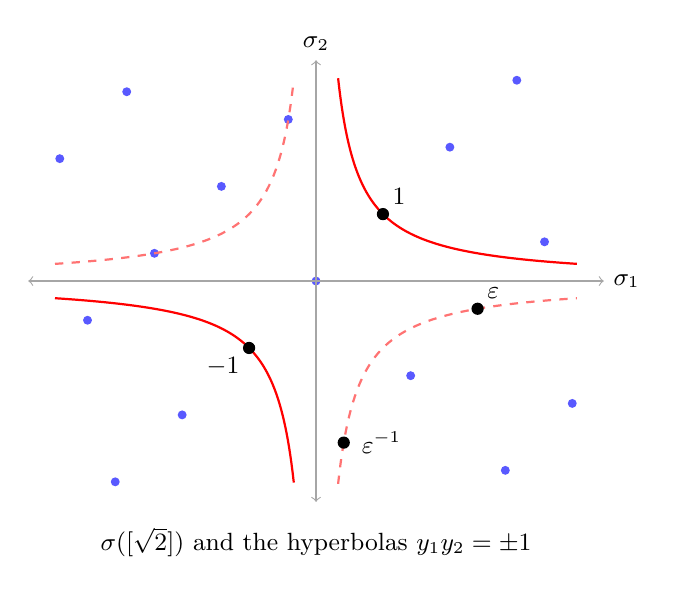
\begin{tikzpicture}[scale=0.85]
		\begin{scope}
			\clip (-4.1,-3.1) rectangle (4.1,3.1);
			\foreach \a in {-8,...,8}{
				\foreach \b in {-8,...,8}{
					\fill[blue!65] ({\a+1.4142*\b},{\a-1.4142*\b}) circle (1.9pt);
				}
			}
			\draw[thick, red, samples=200, domain=0.33:3.9] plot ({\x},{1/\x});
			\draw[thick, red, samples=200, domain=-3.9:-0.33] plot ({\x},{1/\x});
			\draw[thick, red!55, dashed, samples=200, domain=0.33:3.9] plot ({\x},{-1/\x});
			\draw[thick, red!55, dashed, samples=200, domain=-3.9:-0.33] plot ({\x},{-1/\x});
		\end{scope}
		\draw[<->, gray!70] (-4.3,0) -- (4.3,0) node[right, black] {\small $\sigma_1$};
		\draw[<->, gray!70] (0,-3.3) -- (0,3.3) node[above, black] {\small $\sigma_2$};
		\fill[black] (1,1) circle (2.6pt) node[above right=0pt] {\small $1$};
		\fill[black] (-1,-1) circle (2.6pt) node[below left=0pt] {\small $-1$};
		\fill[black] (2.4142,-0.4142) circle (2.6pt) node[above right=0pt] {\small $\varepsilon$};
		\fill[black] (0.4142,-2.4142) circle (2.6pt) node[right=3pt] {\small $\varepsilon^{-1}$};
		\node at (0,-3.9) {\small $\sigma(\Z[\sqrt2])$ and the hyperbolas $y_1y_2 = \pm 1$};
	\end{tikzpicture}
\end{center}

Here $\varepsilon = 1+\sqrt2$ has $\sigma(\varepsilon) = (1+\sqrt2,\,1-\sqrt2)\approx(2.414,-0.414)$, lying on the dashed branch $y_1y_2 = -1$ because $\Nm(\varepsilon) = -1$; its inverse $\varepsilon^{-1} = \sqrt2-1$ has $\sigma(\varepsilon^{-1}) \approx (0.414,-2.414)$. The square $\varepsilon^2 = 3+2\sqrt2$ lands at $(5.83, 0.17)$ on the solid hyperbola $y_1y_2 = 1$, off the right-hand edge of the picture. As $n$ increases, $\sigma(\varepsilon^n)$ marches off along the hyperbolas, hugging the axes ever more closely -- and \emph{every} lattice point on either hyperbola is one of these.

We can prove the rank-$1$ case of Dirichlet's theorem directly, and the proof is instructive.

\begin{theorem}[Pell]\label{nf-thm:pell}
	Let $K = \Q(\sqrt d)$ with $d > 0$ squarefree. Then $\OO_K^\times$ is infinite. Equivalently, $x^2-dy^2 = 1$ has infinitely many integer solutions.
\end{theorem}

\begin{proof}
	Recall $\sigma(x) = (x,\bar x)$ and $\covol(\sigma(\OO_K)) = \abs{d_K}^{1/2}$. For $t > 0$ let
	$$S_t = \left\{(y_1,y_2) \in \R^2 : \abs{y_1}\le t,\ \abs{y_2}\le \abs{d_K}^{1/2}/t\right\},$$
	a closed convex symmetric rectangle whose area is $4\abs{d_K}^{1/2}$, that is, $2^2\covol(\sigma(\OO_K))$. By Minkowski's theorem there is a nonzero $\alpha_t \in \OO_K$ with $\sigma(\alpha_t)\in S_t$, and then
	$$1 \le \abs{\Nm(\alpha_t)} = \abs{y_1y_2} \le \abs{d_K}^{1/2}.$$
	We now produce infinitely many distinct such $\alpha$. Having chosen $t_1 > t_2 > \dots > t_N > 0$, the set $S_{t_N}\cap\sigma(\OO_K)$ is finite (compact meets discrete), and every element of it has nonzero first coordinate (as $\sigma_1$ is injective and $\alpha \neq 0$); so we may choose $t_{N+1} > 0$ smaller than all of these first coordinates in absolute value. Then $\alpha_{t_{N+1}}$ is different from all previous $\alpha_{t_i}$.

	So there are infinitely many $\alpha \in \OO_K$ with $1 \le \abs{\Nm(\alpha)}\le\abs{d_K}^{1/2}$. By pigeonhole some value $m$ is attained infinitely often; and since there are only finitely many ideals of norm $\abs m$ (Corollary \ref{cor:normbounds}), some ideal $(\beta)$ arises as $(\alpha)$ for infinitely many $\alpha$. For any two such, $\alpha/\alpha'$ is a unit, and distinct $\alpha$ give distinct units. So $\OO_K^\times$ is infinite.

	Finally, $\OO_K^\times$ infinite gives a unit $u \neq \pm1$ with $\Nm(u) = \pm1$; then $u^2$ has norm $1$, and writing $u^2 = x+y\sqrt d$ (or $\tfrac12(x+y\sqrt d)$, in which case take $u^6$) gives infinitely many solutions of $x^2-dy^2=1$ from the powers of $u^2$.
\end{proof}

\begin{corollary}
	$\OO_K^\times = \{\pm\varepsilon^n : n \in \Z\}$ for some $\varepsilon$.
\end{corollary}

\begin{proof}
	Identify $K$ with $\sigma_1(K)\subseteq\R$. By the theorem there is a unit $u \neq \pm1$, and $\abs u \neq 1$ (since $\abs u = 1$ with $u$ real forces $u = \pm1$); replacing $u$ by $u^{-1}$ if necessary, $E := \abs u > 1$. The set
	$$\left\{\alpha \in \OO_K : \Nm(\alpha) = \pm1,\ 1 < \abs{\alpha}\le E\right\}$$
	is finite, since $\OO_K$ is discrete in $\R^2$ and this set has bounded coordinates ($\abs\alpha \le E$ and $\abs{\bar\alpha} = 1/\abs\alpha \le 1$). It is nonempty (it contains $u$ or $-u$), so choose $\varepsilon$ in it with $\abs\varepsilon$ minimal, and replace $\varepsilon$ by $-\varepsilon$ if needed so that $\varepsilon > 1$.

	Now let $v \in \OO_K^\times$ with $v > 0$; we claim $v = \varepsilon^N$ for some $N \in \Z$. Write $\log v/\log\varepsilon = N + \gamma$ with $N \in \Z$ and $0 \le \gamma < 1$. Then $w = v\varepsilon^{-N}$ is a unit with $1 \le w = \varepsilon^{\gamma} < \varepsilon$, so by minimality $w = 1$, i.e.\ $\gamma = 0$. Since every unit is $\pm$ a positive one, we are done.
\end{proof}

\subsection{Finding Fundamental Units}

Locating $\varepsilon$ in practice is a matter of searching, and the search can be made short by the following observation: if $\varepsilon = a+b\sqrt d > 1$ is a unit with $\bar\varepsilon = \pm\varepsilon^{-1}$, then $\abs{\bar\varepsilon}<1$, so
$$2a = \varepsilon+\bar\varepsilon > 0 \quad\text{and}\quad 2b\sqrt d = \varepsilon - \bar\varepsilon > 0,$$
so $a, b > 0$. Hence the fundamental unit is the one with smallest positive $b$, and we can simply try $b = 1, 2, 3, \dots$ and test whether $db^2\pm1$ (or $db^2\pm4$) is a square.

\begin{example}
	Let $d = 2$. Guess $\varepsilon = 1+\sqrt2$, which has $\Nm(\varepsilon) = -1$, so it is a unit. It is fundamental: any smaller unit $u = a+b\sqrt2 > 1$ would have $a, b \geq 1$ by the above, hence $u \geq 1+\sqrt2 = \varepsilon$. So $\OO_{\Q(\sqrt2)}^\times = \{\pm(1+\sqrt2)^n\}$ and $R_K = \log(1+\sqrt2) \approx 0.881$.
\end{example}

\begin{example}
	Let $d = 11$, so $\OO_K = \Z[\sqrt{11}]$. Trying $b = 1,2,3$: $11-1 = 10$, $11+1=12$, $44\pm1$, $99+1 = 100 = 10^2$. So $\varepsilon^{-1} = 10-3\sqrt{11}$ has norm $100-99=1$ and $\varepsilon = 10+3\sqrt{11}\approx 19.95$ is a unit.

	Let us verify it is fundamental without appealing to the search. Suppose $u = a+b\sqrt{11}$ is a unit with $1 < u < \varepsilon$. If $\Nm(u) = -1$ then $a^2-11b^2 = -1$, so $a^2\equiv-1\pmod{11}$; but $-1$ is not a square mod $11$ (the squares are $1,3,4,5,9$). So $\Nm(u) = 1$ and $\bar u = u^{-1}$, giving $0 < \bar u < 1$. Adding the inequalities $1 < u < 10+3\sqrt{11}$ and $-1 < -\bar u < 0$:
	$$0 < u - \bar u = 2b\sqrt{11} < 10+3\sqrt{11} < 7\sqrt{11},$$
	so $b \in \{1,2,3\}$. But $11b^2+1 \in \{12, 45, 100\}$ and only $100$ is a square, forcing $u = \varepsilon$. So $\varepsilon$ is fundamental.
\end{example}

\begin{example}
	Some fundamental units, to give a sense of how erratically they grow:
	$$\begin{array}{c|cccccc}
		d & 2 & 3 & 5 & 6 & 7 & 11\\\hline
		\varepsilon & 1+\sqrt2 & 2+\sqrt3 & \tfrac12(1+\sqrt5) & 5+2\sqrt6 & 8+3\sqrt7 & 10+3\sqrt{11}
	\end{array}$$
	$$\begin{array}{c|cccc}
		d & 13 & 19 & 31 & 46\\\hline
		\varepsilon & \tfrac12(3+\sqrt{13}) & 170+39\sqrt{19} & 1520+273\sqrt{31} & 24335+3588\sqrt{46}
	\end{array}$$
	The case $d = 5$ is the golden ratio $\varphi$, with $\varphi^2 = \varphi+1$ and $\Nm(\varphi) = -1$. The jump at $d = 19$ and again at $d = 46$ is typical: the size of $\varepsilon$ is roughly $e^{R_K}$, and the regulator behaves very irregularly.
\end{example}

\begin{example}[A Cubic Field]
	Let $K = \Q(\sqrt[3]2)$, with signature $(1,1)$, so the unit rank is $r+s-1 = 1$ and $\mu_K = \{\pm1\}$ (as $K \subseteq \R$). Consider
	$$\varepsilon = \sqrt[3]2 - 1.$$
	Its minimal polynomial is $(x+1)^3-2 = x^3+3x^2+3x-1$, whose constant term is $-1$, so $\Nm(\varepsilon) = (-1)^3(-1) = 1$ and $\varepsilon$ is a unit. In fact it is fundamental, so
	$$\OO_{\Q(\sqrt[3]2)}^\times = \left\{\pm\left(\sqrt[3]2-1\right)^n : n \in \Z\right\}, \qquad R_K = \log\frac{1}{\sqrt[3]2-1} \approx 1.347.$$
	Note that $\varepsilon \approx 0.26 < 1$, so it is $\varepsilon^{-1} = 1 + \sqrt[3]2+\sqrt[3]4 \approx 3.85$ that is the `large' generator; and $\ell(\varepsilon) = (\log\abs\varepsilon, -\log\abs{\varepsilon})$ since the two coordinates must sum to zero.
\end{example}

\begin{remark}[Continued Fractions]
	There is a systematic algorithm. Every real number has a continued fraction expansion
	$$t = a_0 + \cfrac{1}{a_1+\cfrac{1}{a_2+\cfrac{1}{a_3+\cdots}}} = [a_0,a_1,a_2,\dots], \qquad a_0 = \lfloor t\rfloor,$$
	and a classical theorem of Lagrange says that $t$ is a quadratic irrational if and only if this expansion is eventually periodic. For $\sqrt d$ the expansion is purely periodic after the first term, say $\sqrt d = [a_0,\overline{a_1,\dots,a_m}]$, and then (this is non-examinable, and should not be quoted in exams) if $p/q = [a_0,a_1,\dots,a_{m-1}]$ in lowest terms, the number $p+q\sqrt d$ is a unit, and is fundamental when $d \equiv 2,3\pmod4$.

	For instance $\sqrt7 = [2,\overline{1,1,1,4}]$, and $[2,1,1,1] = 2 + \cfrac{1}{1+\cfrac{1}{1+\cfrac11}} = \tfrac83$, giving $8+3\sqrt7$ with $(8+3\sqrt7)(8-3\sqrt7) = 64-63 = 1$. This algorithm runs in time polynomial in $R_K$, but \emph{not} in $\log\abs{d_K}$; no polynomial-time algorithm is known, and the difficulty is closely related to the erratic growth in the table above.
\end{remark}

\section{Diophantine Applications}\label{sec:applications}

Having built the machinery, let us see it pay for itself. The pattern in each case is the same: an equation over $\Z$ factorises in $\OO_K$ for a suitable $K$, unique factorisation of \emph{ideals} lets us conclude that each factor is (say) a perfect cube as an ideal, and then the class group tells us whether we may promote this to a statement about elements.

The following two observations are what make the pattern work.

\begin{lemma}\label{lem:coprimepower}
	Let $\fa, \fb \trianglelefteq \OO_K$ be coprime nonzero ideals (that is, $\fa+\fb = \OO_K$) with $\fa\fb = \fc^{\,m}$ for some ideal $\fc$ and $m \geq 1$. Then $\fa = \fd^{\,m}$ and $\fb = \fe^{\,m}$ for some ideals $\fd, \fe$.
\end{lemma}

\begin{proof}
	Write $\fa = \prod_\fp\fp^{a_\fp}$ and $\fb = \prod_\fp\fp^{b_\fp}$. Coprimality says no $\fp$ has both $a_\fp > 0$ and $b_\fp > 0$. The hypothesis says $a_\fp+b_\fp \equiv 0 \pmod m$ for every $\fp$, so for each $\fp$ one of $a_\fp, b_\fp$ is zero and the other is divisible by $m$. Take $\fd = \prod_\fp\fp^{a_\fp/m}$ and $\fe = \prod_\fp \fp^{b_\fp/m}$.
\end{proof}

\begin{lemma}\label{lem:coprimeclass}
	Suppose $\gcd(m, h_K) = 1$ and $\fd \trianglelefteq \OO_K$ is an ideal with $\fd^{\,m}$ principal. Then $\fd$ is principal.
\end{lemma}

\begin{proof}
	In $\Cl_K$ we have $[\fd]^m = 1$, so the order of $[\fd]$ divides $m$; it also divides $h_K = \abs{\Cl_K}$ by Lagrange. As $\gcd(m,h_K)=1$, the order is $1$.
\end{proof}

\subsection{Sums of Two Squares}

The oldest application, and still the prettiest.

\begin{theorem}[Fermat]\label{nf-thm:twosquares}
	An odd prime $p$ is a sum of two integer squares if and only if $p \equiv 1 \pmod 4$, and then the representation is unique up to signs and order.
\end{theorem}

\begin{proof}
	Work in $\OO_{\Q(i)} = \Z[i]$, which has $d_K = -4$ and $C_K = \tfrac2\pi\cdot2 < 2$, so $h_K = 1$ and $\Z[i]$ is a PID. Note $\Nm(a+bi) = a^2+b^2$.

	If $p = a^2+b^2$ then modulo $4$ the right-hand side is $0, 1$ or $2$, and $p$ is odd, so $p \equiv 1 \pmod 4$.

	Conversely suppose $p \equiv 1\pmod 4$. Then $-1$ is a quadratic residue mod $p$ (as the group $\F_p^\times$ is cyclic of order $p-1 \equiv 0 \bmod 4$, so contains an element of order $4$), so $x^2+1$ has a root mod $p$ and factors as $(x-r)(x+r)$. By Dedekind's criterion, $p$ splits: $(p) = \fp\bar\fp$ with $\Nm(\fp) = p$. Since $\Z[i]$ is a PID, $\fp = (a+bi)$ for some $a,b$, and $p = \Nm(\fp) = a^2+b^2$.

	For uniqueness, a representation $p = a^2+b^2$ gives $(p) = (a+bi)(a-bi)$, a factorisation into primes of norm $p$; by unique factorisation these must be $\fp$ and $\bar\fp$ in some order, so $a+bi$ is an associate of $a'+b'i$ or of $a'-b'i$, and the units of $\Z[i]$ are $\pm1,\pm i$, which permute $(a,b)$ up to signs and order.
\end{proof}

\begin{example}
	$5 = 1^2+2^2$, $13 = 2^2+3^2$, $17 = 1^2+4^2$, $29 = 2^2+5^2$; whereas $3, 7, 11, 19$ are not sums of two squares. Note $2 = 1^2+1^2$ is the ramified case: $(2) = (1+i)^2$ up to units.
\end{example}

\begin{corollary}
	A positive integer $n$ is a sum of two squares if and only if every prime $q \equiv 3 \pmod 4$ divides $n$ to an even power.
\end{corollary}

\begin{proof}
	$n$ is a sum of two squares if and only if $n = \Nm(\alpha)$ for some $\alpha \in \Z[i]$, i.e.\ $n = \Nm(\fa)$ for some ideal $\fa$ (using $h_K = 1$). Now $\Nm$ is multiplicative and, by Proposition \ref{prop:quadsplit}, the primes of $\Z[i]$ have norms: $2$ (from $(2) = (1+i)^2$), $p$ and $p$ (for $p \equiv 1 \bmod 4$, which splits), and $q^2$ (for $q\equiv3\bmod4$, which is inert). So the norms of ideals are exactly the integers in which each $q \equiv 3\pmod 4$ appears with even exponent.
\end{proof}

\begin{example}[The Form $x^2+2y^2$]
	The same argument runs in $\Z[\sqrt{-2}]$, which is also a PID (its Minkowski constant is $\tfrac2\pi\sqrt8 \approx 1.80 < 2$). An odd prime $p$ is of the form $x^2+2y^2$ if and only if $p$ splits in $\Q(\sqrt{-2})$, which by Proposition \ref{prop:quadsplit} happens exactly when $\legendre{-2}{p} = 1$, that is, when
	$$p \equiv 1, 3 \pmod 8.$$
	So $3 = 1+2$, $11 = 9+2$, $17 = 9+8$, $19 = 1+18$, whereas $5, 7, 13, 23$ are not of this form. The reader may enjoy checking that the same method with $\Z[\omega]$, $\omega = \tfrac12(-1+\sqrt{-3})$, gives: $p$ is of the form $x^2+xy+y^2$ if and only if $p \equiv 1 \pmod 3$.
\end{example}

\begin{remark}
	It is essential here that the relevant ring has class number one. For $x^2+5y^2$ the class number is $2$, and the correct statement splits into two cases according to the ideal class: an odd prime $p \neq 5$ is of the form $x^2+5y^2$ if $p \equiv 1,9 \pmod{20}$, and of the form $2x^2+2xy+3y^2$ -- the other reduced quadratic form of discriminant $-20$ -- if $p \equiv 3,7\pmod{20}$. This is exactly the phenomenon the class group was invented to describe.
\end{remark}

\subsection{Mordell Equations}

The equation $y^2 = x^3+k$ is called a \vocab{Mordell equation}. Mordell proved that it has only finitely many integer solutions for each $k \neq 0$, but finding them is another matter; in favourable cases number fields do it in a page.

\begin{theorem}\label{thm:mordell2}
	The only integer solutions of $y^2 = x^3 - 2$ are $(x,y) = (3,\pm5)$.
\end{theorem}

\begin{proof}
	Write the equation as $y^2 + 2 = x^3$ and work in $K = \Q(\sqrt{-2})$, where $\OO_K = \Z[\sqrt{-2}]$, $d_K = -8$, $\Nm(a+b\sqrt{-2}) = a^2+2b^2$ and $\OO_K^\times = \{\pm1\}$. Since $C_K = \tfrac2\pi\sqrt8 \approx 1.80 < 2$, we have $h_K = 1$.

	\emph{Step 1: $y$ is odd.} If $y$ were even then $x^3 = y^2+2 \equiv 2 \pmod 4$, so $x^3$ is even, hence $x$ is even and $8 \mid x^3$ -- contradicting $x^3 \equiv 2\pmod4$.

	\emph{Step 2: the ideals $(y+\sqrt{-2})$ and $(y-\sqrt{-2})$ are coprime.} Suppose a prime $\fp$ divides both. Then $\fp$ divides their difference $(2\sqrt{-2}) = (\sqrt{-2})^3$, so $\fp = (\sqrt{-2})$, the unique prime above $2$. Then $\fp \mid (y+\sqrt{-2})$ gives $\fp \mid (y)$, so $2 = \Nm(\fp)$ divides $\Nm((y)) = y^2$, making $y$ even -- contradicting Step 1.

	\emph{Step 3: cubes.} We have $(y+\sqrt{-2})(y-\sqrt{-2}) = (x)^3$ with the factors coprime, so by Lemma \ref{lem:coprimepower} there is an ideal $\fd$ with $(y+\sqrt{-2}) = \fd^3$. As $h_K = 1$, $\fd = (\gamma)$ is principal, so $y+\sqrt{-2} = u\gamma^3$ for a unit $u = \pm1$; and $\pm1 = (\pm1)^3$, so absorbing the unit into $\gamma$,
	$$y+\sqrt{-2} = \left(a+b\sqrt{-2}\right)^3 \quad\text{for some } a, b \in \Z.$$

	\emph{Step 4: solve.} Expanding,
	$$\left(a+b\sqrt{-2}\right)^3 = a^3 - 6ab^2 + \left(3a^2b - 2b^3\right)\sqrt{-2},$$
	so comparing coefficients of $\sqrt{-2}$,
	$$1 = 3a^2b - 2b^3 = b\left(3a^2-2b^2\right).$$
	Hence $b \mid 1$. If $b = 1$ then $3a^2-2 = 1$, so $a = \pm1$; if $b = -1$ then $3a^2-2 = -1$, so $3a^2 = 1$, impossible. So $b = 1$, $a = \pm1$, and
	$$y = a^3-6ab^2 = a^3 - 6a = \mp 5,$$
	giving $y = \pm5$ and $x^3 = 25+2 = 27$, so $x = 3$.
\end{proof}

Now an example where the class group genuinely intervenes.

\begin{theorem}\label{thm:mordell5}
	The equation $y^2 = x^3-5$ has no integer solutions.
\end{theorem}

\begin{proof}
	Write $y^2+5 = x^3$ and work in $K = \Q(\sqrt{-5})$, so $\OO_K = \Z[\sqrt{-5}]$, $\OO_K^\times = \{\pm1\}$ and $h_K = 2$ by Example \ref{ex:cl5}.

	\emph{Step 1: $x$ is odd.} If $x$ were even then $8 \mid x^3$, so $y^2 \equiv -5\equiv 3\pmod 8$; but squares mod $8$ are $0,1,4$.

	\emph{Step 2: coprimality.} Suppose a prime $\fp$ divides $(y+\sqrt{-5})$ and $(y-\sqrt{-5})$. Then $\fp \mid (2\sqrt{-5})$, so $\fp$ is the prime $\fp_2 = (2,1+\sqrt{-5})$ above $2$ or the prime $\fp_5 = (\sqrt{-5})$ above $5$.

	If $\fp = \fp_2$ then $\fp_2 \mid (y+\sqrt{-5})(y-\sqrt{-5}) = (x)^3$, so $\fp_2\mid(x)$ and $2 = \Nm(\fp_2)$ divides $x^2$, making $x$ even -- contradicting Step 1.

	If $\fp = \fp_5$ then similarly $5 \mid x^2$, so $5\mid x$ and $125 \mid x^3$. Then $y^2 = x^3-5 \equiv -5 \pmod{25}$, so $5 \mid y^2$, so $5\mid y$ and $25 \mid y^2$; but then $25 \mid x^3-y^2 = 5$, absurd.

	\emph{Step 3: cubes.} As before $(y+\sqrt{-5}) = \fd^3$ for some ideal $\fd$. Now $\gcd(3, h_K) = \gcd(3,2) = 1$, so Lemma \ref{lem:coprimeclass} applies: $\fd = (\gamma)$ is principal. Absorbing the unit $\pm1 = (\pm1)^3$,
	$$y+\sqrt{-5} = \left(a+b\sqrt{-5}\right)^3 = a^3-15ab^2 + \left(3a^2b-5b^3\right)\sqrt{-5}.$$

	\emph{Step 4: solve.} Comparing coefficients, $1 = b(3a^2-5b^2)$, so $b = \pm1$. If $b = 1$ then $3a^2 = 6$, so $a^2 = 2$, impossible; if $b=-1$ then $3a^2 = 4$, impossible. So there are no solutions.
\end{proof}

\begin{remark}
	Step 3 is exactly where the class group earns its keep, and it is where the argument would break down if $3$ divided $h_K$. If instead we had tried this with $\Q(\sqrt{-26})$, whose class number is $6$, the argument would fail -- and indeed $y^2 = x^3-26$ \emph{does} have solutions, namely $(3,\pm1)$ and $(35,\pm207)$. Similarly, one must never forget the unit-absorbing step: it works here only because the unit group is $\{\pm1\}$ and every unit is a cube. Over a real quadratic field, with its infinite unit group, considerably more care is needed.
\end{remark}

\subsection{Cyclotomic Fields and Fermat's Last Theorem}

Kummer's original motivation for inventing ideal numbers was Fermat's equation
$$x^p+y^p = z^p, \qquad p \text{ an odd prime}.$$
In $\Q(\zeta_p)$ the left-hand side factors completely:
$$x^p+y^p = \prod_{i=0}^{p-1}\left(x+\zeta_p^{\,i}y\right).$$
Suppose $x,y,z$ are pairwise coprime integers with $p \nmid xyz$ (this is \vocab{Case I}). One checks that the ideals $(x+\zeta_p^{\,i}y)$ are pairwise coprime, so their product being $(z)^p$ forces
$$\left(x+\zeta_py\right) = \fa^p$$
for some ideal $\fa$, by Lemma \ref{lem:coprimepower}. So far this is exactly the Mordell argument. The step that fails in general is the promotion of $\fa^p$ principal to $\fa$ principal: this needs $p \nmid h_{\Q(\zeta_p)}$.

\begin{definition}[Regular Prime]
	An odd prime $p$ is \vocab{regular} if $p \nmid h_{\Q(\zeta_p)}$.
\end{definition}

\begin{theorem}[Kummer]
	If $p$ is a regular prime then $x^p+y^p = z^p$ has no solutions in nonzero integers.
\end{theorem}

The remaining work, which we do not do here, is to control the units of $\Z[\zeta_p]$ (there is a lemma of Kummer saying that every unit is $\zeta_p^{\,a}$ times a real unit), and to handle Case II where $p \mid xyz$ by a descent.

The smallest irregular prime is $37$, and the first few are $37, 59, 67, 101, 103, 131, 149, 157$. Kummer gave a beautiful criterion: $p$ is irregular precisely when $p$ divides the numerator of one of the Bernoulli numbers $B_2, B_4, \dots, B_{p-3}$. It is known that infinitely many primes are irregular; whether infinitely many are regular is, remarkably, still open, although heuristics suggest about $e^{-1/2} \approx 61\%$ of primes should be.

\begin{example}
	For $p \le 19$ one has $h_{\Q(\zeta_p)} = 1$, so all these primes are regular and Fermat's equation has no solutions for these exponents. The first failure of $h = 1$ is $p = 23$, where $h_{\Q(\zeta_{23})} = 3$; but $23 \nmid 3$, so $23$ is still regular.
\end{example}

\begin{remark}
	Of course, Fermat's Last Theorem is now a theorem of Wiles for all $n \geq 3$, by a route -- modular forms and Galois representations -- with no visible relation to Kummer's. But Kummer's approach is the origin of algebraic number theory, and the class group of $\Q(\zeta_p)$ remains an object of intense study; the Herbrand--Ribet theorem, for instance, describes exactly which pieces of it are nontrivial in terms of Bernoulli numbers.
\end{remark}

\section{The Dedekind Zeta Function}\label{sec:zeta}

This final section is non-examinable. Its purpose is to show that the two invariants we have worked so hard to compute -- the class number $h_K$ and the regulator $R_K$ -- are not isolated curiosities, but appear together as the residue of a single analytic function; and to use this to prove Dirichlet's theorem on primes in arithmetic progressions, a result about $\Z$ whose only known proofs go through number fields.

\subsection{Dirichlet Series}

Euler's proof that there are infinitely many primes runs as follows. By unique factorisation in $\Z$,
$$\prod_{p \text{ prime}}\left(1-\frac1p\right)^{-1} = \prod_p\left(1+\frac1p+\frac{1}{p^2}+\dots\right) = \sum_{n\ge1}\frac1n,$$
since each $n$ arises exactly once when the product is expanded. The right-hand side diverges, so the product cannot be finite. This is already better than Euclid's proof, because it says something quantitative; but it says nothing about primes in a fixed congruence class, since there is no such product formula for $\prod_{p\equiv a\, (q)}$. Dirichlet's idea was to introduce a variable.

\begin{definition}[Riemann Zeta Function]
	For $s \in \C$ with $\re(s) > 1$, define $\displaystyle\zeta(s) = \sum_{n\ge1}n^{-s}$.
\end{definition}

More generally, a \vocab{Dirichlet series} is a function of the form $\sum_{n\ge1}a_nn^{-s}$ for a sequence $(a_n)$ of complex numbers. Convergence is controlled by the partial sums of the $a_n$.

\begin{lemma}\label{lem:dirichletconv}
	Suppose $a_1+\dots+a_N = O(N^r)$ for some $r \in \R$. Then $\sum_{n\ge1}a_nn^{-s}$ converges to a holomorphic function on $\re(s) > r$.
\end{lemma}

\begin{proof}
	Write $T(N) = a_1+\dots+a_N$, so $\abs{T(N)}\le BN^r$ for some constant $B$. Abel summation gives
	$$\sum_{n=1}^Na_nn^{-s} = \sum_{n=1}^{N-1}T(n)\left(n^{-s}-(n+1)^{-s}\right) + \frac{T(N)}{N^s}.$$
	If $\re(s) > r$ then $\abs{T(N)/N^s} \le B N^{r-\re(s)}\to0$, so it suffices to show that the sum $\sum_n T(n)\left(n^{-s}-(n+1)^{-s}\right)$ converges absolutely. Now
	$$n^{-s}-(n+1)^{-s} = s\int_n^{n+1}\frac{\dd x}{x^{s+1}},$$
	and $n^r \le x^r$ for $x \in [n,n+1]$ when $r \geq 0$ (and $n^r \le (x-1)^r$ otherwise, which is handled the same way), so
	$$\abs{T(n)}\abs{n^{-s}-(n+1)^{-s}} \le B\abs{s}\int_n^{n+1}\frac{\dd x}{x^{\re(s)+1-r}},$$
	and summing over $n$ gives a convergent integral $\int_1^\infty x^{r-\re(s)-1}\dd x$. Holomorphy follows since the convergence is locally uniform.
\end{proof}

\begin{proposition}\label{prop:zetaprops}
	\begin{enumerate}[label=(\roman*)]
		\item $\zeta(s)$ converges to a holomorphic function on $\re(s)>1$;
		\item on that region, $\displaystyle\zeta(s) = \prod_{p}\left(1-p^{-s}\right)^{-1}$, the \vocab{Euler product};
		\item $\zeta(s) - \frac1{s-1}$ extends holomorphically to $\re(s)>0$. In particular $\zeta$ has a simple pole at $s=1$ with residue $1$.
	\end{enumerate}
\end{proposition}

\begin{proof}
	(i) is Lemma \ref{lem:dirichletconv} with $a_n = 1$, so $T(N) = N = O(N)$.

	(ii) Let $p_1,\dots,p_m$ be the first $m$ primes and $X$ the set of positive integers all of whose prime factors lie among them. Expanding geometric series and using unique factorisation, $\prod_{i\le m}(1-p_i^{-s})^{-1} = \sum_{n\in X}n^{-s}$, so
	$$\left|\zeta(s) - \prod_{i\le m}\left(1-p_i^{-s}\right)^{-1}\right| = \left|\sum_{n\notin X}n^{-s}\right|\le\sum_{n > m}n^{-\re(s)} \to 0,$$
	using $1,\dots,m \in X$.

	(iii) Since $\frac1{s-1} = \sum_{n\ge1}\int_n^{n+1}t^{-s}\dd t$, we get
	$$\zeta(s)-\frac1{s-1} = \sum_{n\ge1}\int_n^{n+1}\left(n^{-s}-t^{-s}\right)\dd t,$$
	and each term is $O(\abs s n^{-\re(s)-1})$ by the mean value theorem, so the sum converges locally uniformly for $\re(s)>0$.
\end{proof}

\subsection{The Dedekind Zeta Function}

The Euler product is exactly the analytic shadow of unique factorisation, so it should have an analogue in any $\OO_K$.

\begin{definition}[Dedekind Zeta Function]
	Let $K$ be a number field. Its \vocab{Dedekind zeta function} is
	$$\zeta_K(s) = \sum_{0 \neq \fa\trianglelefteq\OO_K}\Nm(\fa)^{-s} = \sum_{n\ge1}\frac{a_n}{n^s}, \qquad a_n = \#\left\{\fa\trianglelefteq\OO_K : \Nm(\fa) = n\right\},$$
	which is a finite count by Corollary \ref{cor:normbounds}.
\end{definition}

\begin{theorem}[Analytic Class Number Formula]\label{thm:acnf}
	Let $K$ be a number field of degree $n$ and signature $(r,s)$. Then
	\begin{enumerate}[label=(\roman*)]
		\item $\zeta_K(s)$ converges to a holomorphic function on $\re(s)>1$;
		\item on that region $\displaystyle\zeta_K(s) = \prod_{\fp}\left(1-\Nm(\fp)^{-s}\right)^{-1}$, the product over nonzero primes of $\OO_K$;
		\item $\zeta_K$ extends meromorphically to $\re(s) > 1 - \tfrac1n$ with a simple pole at $s = 1$ of residue
		$$\Res_{s=1}\zeta_K(s) = \frac{2^{r}(2\pi)^{s}\,h_K\,R_K}{\abs{\mu_K}\,\abs{d_K}^{1/2}}.$$
	\end{enumerate}
\end{theorem}

Part (ii) is a formal consequence of unique factorisation of ideals and multiplicativity of the norm, exactly as in Proposition \ref{prop:zetaprops}(ii). Parts (i) and (iii) follow from Lemma \ref{lem:dirichletconv} together with the counting estimate
$$a_1+\dots+a_N = \frac{2^{r}(2\pi)^{s}h_KR_K}{\abs{\mu_K}\abs{d_K}^{1/2}}\cdot N + O\!\left(N^{1-1/n}\right),$$
which is proved by counting lattice points of bounded norm in each ideal class -- a substantial but entirely geometric computation of the same flavour as the Minkowski bound.

It is worth pausing over this formula. On the left is an analytic object built out of counting ideals; on the right sit \emph{every} invariant we have studied: the class number, the regulator, the number of roots of unity, the discriminant and the signature. It is one of the most beautiful formulae in mathematics, and it is the prototype for a vast web of conjectures (Birch--Swinnerton-Dyer, Bloch--Kato) relating special values of $L$-functions to arithmetic invariants.

\begin{example}
	For $K = \Q$ we have $r = 1, s= 0, h = 1, R = 1, \abs{\mu} = 2, \abs{d} = 1$, and the formula reads $\Res_{s=1}\zeta(s) = 2/2 = 1$, agreeing with Proposition \ref{prop:zetaprops}(iii).
\end{example}

\subsection{Factorisation and Dirichlet $L$-functions}

For $K \neq \Q$ the function $\zeta_K$ factors, and the factors are interesting. Take $K = \Q(\sqrt d)$ quadratic with $D = d_K$. Grouping the Euler product by rational primes and using Proposition \ref{prop:quadsplit}:
\begin{itemize}
	\item if $p$ ramifies, $(p)=\fp^2$ with $\Nm(\fp) = p$, contributing $\left(1-p^{-s}\right)^{-1}$;
	\item if $p$ is inert, $\Nm(\fp)=p^2$, contributing $\left(1-p^{-2s}\right)^{-1} = \left(1-p^{-s}\right)^{-1}\left(1+p^{-s}\right)^{-1}$;
	\item if $p$ splits, two primes of norm $p$, contributing $\left(1-p^{-s}\right)^{-2}$.
\end{itemize}
In every case the contribution is $\left(1-p^{-s}\right)^{-1}\left(1-\chi_D(p)p^{-s}\right)^{-1}$ where
$$\chi_D(p) = \begin{cases}0 & p \text{ ramifies},\\ -1 & p \text{ inert},\\ +1 & p \text{ splits}\end{cases} \qquad\left( = \legendre{D}{p} \text{ for odd } p\right).$$
Extending $\chi_D$ multiplicatively to all $n \geq 1$ and setting
$$L(\chi_D,s) = \prod_p\left(1-\chi_D(p)p^{-s}\right)^{-1} = \sum_{n\ge1}\frac{\chi_D(n)}{n^s},$$
we have shown
$$\zeta_{\Q(\sqrt d)}(s) = \zeta(s)\,L(\chi_D,s).$$

\begin{definition}[Dirichlet Character]
	A \vocab{Dirichlet character} of modulus $q$ is a function $\chi : \Z \to \C$ of the form
	$$\chi(n) = \begin{cases}\omega(n \bmod q) & \gcd(n,q)=1,\\ 0 & \text{otherwise},\end{cases}$$
	for a group homomorphism $\omega : (\Z/q\Z)^\times \to \C^\times$. It is \vocab{trivial} if $\omega \equiv 1$.
\end{definition}

Such $\chi$ are completely multiplicative, so $L(\chi,s) = \prod_p(1-\chi(p)p^{-s})^{-1} = \sum_n\chi(n)n^{-s}$ makes sense for $\re(s)>1$.

\begin{theorem}
	For $d$ squarefree with $D = d_{\Q(\sqrt d)}$, the function $\chi_D$ is a Dirichlet character of modulus $\abs{D}$.
\end{theorem}

The proof is a case analysis using quadratic reciprocity; in fact the statement is essentially \emph{equivalent} to quadratic reciprocity, which is a striking way to view that theorem: the law of quadratic reciprocity is the assertion that the splitting behaviour of $p$ in $\Q(\sqrt d)$ depends only on $p$ modulo $d_K$.

\begin{example}
	Let $K = \Q(i)$, so $D = -4$. For odd $p$, $\chi_{-4}(p) = \legendre{-1}{p} = (-1)^{(p-1)/2}$, and $\chi_{-4}(2) = 0$ since $2$ ramifies. So $\chi_{-4}(n) = (-1)^{(n-1)/2}$ for $n$ odd and $0$ for $n$ even, and
	$$L(\chi_{-4},s) = 1-\frac1{3^s}+\frac1{5^s}-\frac1{7^s}+\dots$$
	Comparing residues at $s = 1$ in $\zeta_{\Q(i)} = \zeta\cdot L(\chi_{-4},\cdot)$ and using Theorem \ref{thm:acnf} with $r=0,s=1,h=1,R=1,\abs\mu = 4,\abs d = 4$:
	$$L(\chi_{-4},1) = \Res_{s=1}\zeta_{\Q(i)}(s) = \frac{(2\pi)\cdot 1\cdot 1}{4\cdot 2} = \frac\pi4,$$
	which is Leibniz's formula $1-\tfrac13+\tfrac15-\tfrac17+\dots = \tfrac\pi4$. The class number formula \emph{proves} Leibniz's series.
\end{example}

\begin{lemma}\label{lem:Lnontrivial}
	If $\chi$ is a nontrivial Dirichlet character, then $L(\chi,s)$ is holomorphic on $\re(s)>0$.
\end{lemma}

\begin{proof}
	By orthogonality of characters of the finite abelian group $(\Z/q\Z)^\times$, applied to the trivial character and $\omega \neq 1$,
	$$\sum_{n = aq+1}^{(a+1)q}\chi(n) = \sum_{u \in (\Z/q\Z)^\times}\omega(u) = 0$$
	for every $a$. Hence the partial sums $\sum_{n\le N}\chi(n)$ are bounded, i.e.\ $O(N^0)$, and Lemma \ref{lem:dirichletconv} applies with $r = 0$.
\end{proof}

\begin{corollary}
	If $D < 0$ is a fundamental discriminant then
	$$L(\chi_D,1) = \frac{2\pi\, h_{\Q(\sqrt D)}}{\abs{\mu_{\Q(\sqrt D)}}\abs{D}^{1/2}} \neq 0.$$
\end{corollary}

\begin{proof}
	Both sides of $\zeta_{\Q(\sqrt D)} = \zeta\cdot L(\chi_D,\cdot)$ have a simple pole at $s=1$; comparing residues and using $\Res_{s=1}\zeta = 1$ together with Theorem \ref{thm:acnf} (with $r=0$, $s=1$, $R = 1$) gives the formula. It is nonzero since $h \geq 1$.
\end{proof}

\subsection{Primes in Arithmetic Progressions}

To handle general moduli we need the cyclotomic analogue of the factorisation above. Let $q \geq 1$, $L = \Q(\zeta_q)$ and $G = \Gal(L/\Q) \cong (\Z/q\Z)^\times$, of order $\varphi(q)$. By Proposition \ref{prop:cyclo}, for $p \nmid q$ the primes above $p$ number $\varphi(q)/f$ and have norm $p^f$, where $f$ is the order of $p$ in $G$. So these primes contribute
$$\left(1-p^{-fs}\right)^{-\varphi(q)/f}$$
to $\zeta_L$. Let $\omega_1 = \mathbbm 1,\omega_2,\dots,\omega_{\varphi(q)}$ be the characters of the abelian group $G$, and $\chi_i$ the corresponding Dirichlet characters mod $q$. Restricted to the cyclic subgroup $\langle p\rangle$ of order $f$, the $\omega_i$ run over the $f$ characters of $\langle p \rangle$, each $\varphi(q)/f$ times; so $\omega_1(p),\dots,\omega_{\varphi(q)}(p)$ are exactly the $f$th roots of unity, each repeated $\varphi(q)/f$ times. Since $1-t^f = \prod_{\gamma^f=1}(1-\gamma t)$, putting $t = p^{-s}$ gives
$$\left(1-p^{-fs}\right)^{-\varphi(q)/f} = \prod_{i=1}^{\varphi(q)}\left(1-\omega_i(p)p^{-s}\right)^{-1}.$$
Multiplying over all $p \nmid q$ and accounting for the finitely many $p \mid q$ by a correction factor $C(s)$ (a finite product of terms $(1-p^{-f_ps})^{-1}$, holomorphic and nonvanishing at $s=1$):
$$\zeta_{\Q(\zeta_q)}(s) = C(s)\prod_{i=1}^{\varphi(q)}L(\chi_i,s) = C'(s)\,\zeta(s)\prod_{i=2}^{\varphi(q)}L(\chi_i,s).$$

\begin{theorem}\label{thm:Lnonzero}
	If $\chi$ is a nontrivial Dirichlet character then $L(\chi,1) \neq 0$.
\end{theorem}

\begin{proof}
	Every nontrivial Dirichlet character mod $q$ is one of the $\chi_i$ above with $i \neq 1$. By Lemma \ref{lem:Lnontrivial}, each such $L(\chi_i,s)$ is holomorphic at $s = 1$. Now compare orders of vanishing at $s = 1$ in the displayed factorisation: the left-hand side has a \emph{simple} pole by Theorem \ref{thm:acnf}, and on the right $\zeta$ contributes a simple pole while $C'$ is holomorphic and nonzero. So $\prod_{i\ge2}L(\chi_i,1)$ must be finite and nonzero, whence each factor is nonzero.
\end{proof}

\begin{theorem}[Dirichlet]\label{thm:primesAP}
	Let $a, q$ be coprime positive integers. Then there are infinitely many primes $p \equiv a \pmod q$.
\end{theorem}

\begin{proof}
	Orthogonality of the columns of the character table of $(\Z/q\Z)^\times$ gives, for any $n$,
	$$\frac{1}{\varphi(q)}\sum_{i=1}^{\varphi(q)}\overline{\chi_i(a)}\chi_i(n) = \begin{cases}1 & n\equiv a \pmod q,\\ 0 & \text{otherwise},\end{cases}$$
	valid even when $\gcd(n,q)>1$ since then every $\chi_i(n) = 0$. Hence for real $s > 1$,
	$$\sum_{p \equiv a\, (q)}p^{-s} = \frac1{\varphi(q)}\sum_{i}\overline{\chi_i(a)}\sum_p\chi_i(p)p^{-s}.$$
	Now expand the logarithm of the Euler product: for $\re(s)>1$,
	$$\log L(\chi,s) = -\sum_p\log\left(1-\chi(p)p^{-s}\right) = \sum_{p}\frac{\chi(p)}{p^s} + \sum_{p,\, m\ge2}\frac{\chi(p^m)}{mp^{ms}},$$
	and the double sum is bounded as $s \to 1^+$, since
	$$\sum_{p,\,m\ge2}p^{-ms} = \sum_p\frac{1}{p^s(p^s-1)} \le \sum_{n\ge2}\frac{1}{n(n-1)} < \infty.$$
	So, up to a bounded function,
	$$\sum_{p\equiv a\,(q)}p^{-s} \sim \frac1{\varphi(q)}\sum_i\overline{\chi_i(a)}\log L(\chi_i,s).$$
	For $i = 1$ we have $L(\chi_1,s) = \zeta(s)\prod_{p\mid q}(1-p^{-s})$, which has a simple pole at $s=1$, so $\log L(\chi_1,s)\sim\log\frac1{s-1}\to\infty$. For $i \geq 2$, Lemma \ref{lem:Lnontrivial} and Theorem \ref{thm:Lnonzero} say $L(\chi_i,s)$ is holomorphic and nonzero at $s = 1$, so $\log L(\chi_i,s)$ stays bounded. Therefore
	$$\sum_{p\equiv a\,(q)}p^{-s} \sim \frac{1}{\varphi(q)}\log\frac1{s-1} \longrightarrow \infty \quad\text{as } s\to1^+,$$
	which is impossible if there are only finitely many such primes.
\end{proof}

The proof gives more than infinitude: the factor $1/\varphi(q)$ says that the primes are \vocab{equidistributed} among the $\varphi(q)$ invertible classes mod $q$, in the sense of Dirichlet density.

\begin{remark}
	This is the tip of a very large iceberg. For $L/\Q$ Galois with group $G$, the zeta function factors as
	$$\zeta_L(s) = \prod_{\rho}L(\rho,s)^{\dim\rho},$$
	the product over irreducible complex representations of $G$, where the $L(\rho,s)$ are \vocab{Artin $L$-functions}; the factorisation mirrors the decomposition of the regular representation, and $L(\mathbbm 1, s) = \zeta(s)$. Artin conjectured that $L(\rho,s)$ is entire for $\rho \neq \mathbbm 1$, which is still open. For one-dimensional $\rho$, matching $L(\rho,s)$ with a Dirichlet $L$-function is the content of class field theory -- the vast generalisation of quadratic reciprocity -- and the higher-dimensional case is the Langlands programme. All of it begins with the observation that unique factorisation of ideals gives an Euler product.
\end{remark}

\section{Further Directions}

We close with a brief and impressionistic look at where the subject goes next; none of this is examinable, but all of it is the natural continuation of what we have done.

\subsection{Class Field Theory}

We saw in Section \ref{sec:cyclo} that the splitting of a prime $q$ in $\Q(\zeta_m)$ depends only on $q$ modulo $m$, and that this fact, restricted to the quadratic subfield of $\Q(\zeta_p)$, \emph{is} quadratic reciprocity. The Kronecker--Weber theorem says that this example is exhaustive:

\begin{theorem}[Kronecker--Weber]
	Every finite abelian extension of $\Q$ is contained in some cyclotomic field $\Q(\zeta_m)$.
\end{theorem}

So the abelian extensions of $\Q$ are completely understood, and splitting in them is always governed by congruence conditions. Class field theory does the same for an arbitrary number field $K$: it classifies the abelian extensions of $K$ in terms of data intrinsic to $K$. The simplest instance is the \vocab{Hilbert class field} $H$ of $K$, the maximal unramified abelian extension, which satisfies
$$\Gal(H/K)\cong\Cl_K, \qquad [H:K] = h_K,$$
and in which a prime $\fp$ of $K$ splits completely if and only if $\fp$ is principal. So the class group -- which we introduced as a measure of the failure of unique factorisation -- turns out to be a Galois group.

\begin{example}
	Take $K = \Q(\sqrt{-5})$, with $h_K = 2$. Its Hilbert class field is $H = K(i) = \Q(i,\sqrt5)$, of degree $2$ over $K$. This gives a slick explanation of the congruence conditions in the remark of Section \ref{sec:applications}: whether $p$ is $x^2+5y^2$ or $2x^2+2xy+3y^2$ is governed by whether $p$ splits completely in $H$.
\end{example}

For $K$ imaginary quadratic there is a beautiful explicit theory -- \vocab{complex multiplication} -- generating the abelian extensions of $K$ using special values of elliptic modular functions, in exact analogy with the way roots of unity, i.e.\ special values of $e^{2\pi iz}$, generate the abelian extensions of $\Q$. Doing the same for a general base field is Hilbert's twelfth problem, and it is still open.

\subsection{How Do Class Groups Behave?}

We computed a handful of class groups, and they looked rather arbitrary. That impression is correct, and it has been made precise. The \vocab{Cohen--Lenstra heuristics} predict, roughly, that the odd part of the class group of a random imaginary quadratic field is a random finite abelian group, weighted inversely by the size of its automorphism group. The predictions are strikingly accurate numerically, and some cases are now theorems; but the basic questions remain hard. It is not known, for instance, whether infinitely many real quadratic fields have class number one, even though numerically they appear to make up more than three quarters of all real quadratic fields.

What \emph{is} known is a strong contrast between the two cases. For imaginary quadratic fields, $h_K \to \infty$ as $\abs{d_K}\to\infty$ -- indeed $h_K \gg \abs{d_K}^{1/2-\varepsilon}$ by Siegel's theorem -- which is why the list of nine class number one fields in Section \ref{sec:computing} is finite. For real quadratic fields the class number formula ties $h_K$ to $h_KR_K$, and the regulator can be enormous (recall the fundamental unit for $d = 46$), so a large $\abs{d_K}$ is perfectly compatible with $h_K = 1$.

\subsection{Beyond Number Fields}

Everything in this course had a geometric shadow. A Dedekind domain is precisely the coordinate ring of a smooth affine curve, and the analogy
$$\Z \longleftrightarrow \F_q[t], \qquad \Q \longleftrightarrow \F_q(t), \qquad \text{number field} \longleftrightarrow \text{function field of a curve}$$
is close enough to be genuinely useful in both directions. Under it, the class group of $\OO_K$ corresponds to the Picard group of a curve, the unit theorem corresponds to a statement about functions with prescribed poles, and the Dedekind zeta function corresponds to the zeta function of a curve over a finite field -- where the Riemann hypothesis is a theorem of Weil.

Finally, the pattern of Section \ref{sec:applications} -- factor a Diophantine equation in a suitable ring, use the class group to control the factors -- is the ancestor of the modern theory. It is superseded by the theory of elliptic curves for equations like $y^2 = x^3+k$, where Mordell's theorem says the rational points form a finitely generated abelian group (a statement whose proof is a descent argument in the same spirit as Dirichlet's unit theorem), and ultimately by the machinery of modular forms and Galois representations that settled Fermat's Last Theorem. But all of it starts here, with the observation that $6 = 2\cdot3 = (1+\sqrt{-5})(1-\sqrt{-5})$.

